
\documentclass[../notes.tex]{subfiles}

\graphicspath{{\subfix{../img/}}}

\begin{document}

\section{ECE568 Computer Security}

\subsection{Refresher \& Introduction}

\begin{blockquote}
    I've found that the way that this course is organized does not lend itself well to well-organized headers and notes. Apologies for the train-of-thought style.
\end{blockquote}


Software systems are ubiquitous and critical. Therefore it is important to learn how to protect against malicious actors. This course covers attack vectors and ways to design software securely



\textbf{Data representation}: It's important to recognize that data is just a collection of bits and it is up to us to tell the computer how it should be interpreted. Oftentimes we can make assumptions, for example assume that an int is an int. But what if we end up being wrong about it? 
Many security exploits rely on data being interpreted in a different way than originally intended.
For example,

\begin{listing}[H]
\begin{minted}{c}
unsigned long int h = 0x6f6c6c6548; // ascii for hello
unsigned long int w = 431316168567; // ascii for world
printf("%s %s", (char*) h, (char*) w);
\end{minted}
\caption{An innocent example of where we should be careful about data representation. This prints hello world}
\end{listing}

This courses makes use of Intel assembler.
TLDR:

\begin{itemize}
  \item 6 General-purpose registers
  \item RAX (64b), EAX(32b), AX(16b), AH/AL(8b), etc
\end{itemize}

Note that the stack grows downwards and the heap grows upwards. Stack overflows can occur and can be a source of vulnerability.


GDB offers some tools for examining stacks

\begin{itemize}
    \item \texttt{break}: create a new breakpoint
    \item \texttt{run}: start a new process
    \item \texttt{where}: list of current stack frames
    \item \texttt{up/down}: move between frames
    \item \texttt{info frame} display info on current frame
    \item \texttt{info args}: list function arguments
    \item \texttt{info locals}: list local variables
    \item \texttt{print}: display a variable
    \item \texttt{x} display contents of memory
\end{itemize}

\begin{itemize}
    \item \texttt{fork}: Creates a new child process by duplicating the parent. The child has its own new unique process ID
    \item \texttt{exec}: Replaces the current process with a new process
\end{itemize}

\marginnote{The fork-exec technique is just a pair of \texttt{fork} and \texttt{exec} system calls to spawn a new program in a new process}



\subsubsection{Security Fundamentals}

The three key components of security are:

\begin{itemize}
    \item Confidentiality: the protection of data/resources from exposure, whether it be the content or the knowledge that the resource exists in the first place. Usually via organizational controls (security training), access rules, and cryptography.
    \item Integrity: Trustworthiness of data (contents, origin). Via monitoring, auditing, and cryptography.
    \item Availability: Ability to access/use a resource as desired. Can be hard to ensure; uptime, etc...
\end{itemize}

Together they form an acryonym: CIA. A system is considered secure if it has all three of these properties for a given time.
The strength of cryptographic systems can be evaluated by the number of bits of entropy or their complexity. For example, a 128-bit key has 2\^128 possible values. This would take a lot of time to break, and a 256-bit key even longer.
Availability is harder to measure quantitatively and is instead traditionally measured qualitatively. For example, a system may be available 99.9\% of the time. But this doesn't really measure w.r.t security.


Some security terms:
\begin{itemize}
    \item Another security concept is the \textbf{threat}, or any method that can breach security.
    \item An exercise of a threat is called an \textbf{exploit}  and a successful exploit causes the system to be compromised. Common threats include internet connections/open ports.
    \item \textbf{Vulnerabilities}  are flaws that that weaken the security of a system and can be difficult to detect. For example an unchecked string copy can cause a buffer overflow and allow an attacker to execute arbitrary code
    \item \textbf{Compromises} are the intersection between threats and Vulnerabilities, i.e. when an attacker matches a threat with a vulnerability (i.e. matching a tool in the attacker's arsenal with a weakness)
    \item \textbf{Trust} : How much exposure a system has to an interface. For example a PC might have a lot of trust in the user.
\end{itemize}

The leading cause of computer security breaches are humans. We are prone to making mistakes.
A general trade-off exists when designing secure systems for humans; the more secure a system becomes the less usable it  tends to be. One way of measuring the quality of a security system is how secure it is while maintaining usability

\subsubsection{Reflections on Trusting Trust}

\begin{blockquote}
    \textbf{Reflections on Trusting Trust} is a paper by Ken Thompson that discusses the trust and security in computing. Cool short read.
\end{blockquote}


\begin{figure}[H]
    \centering
    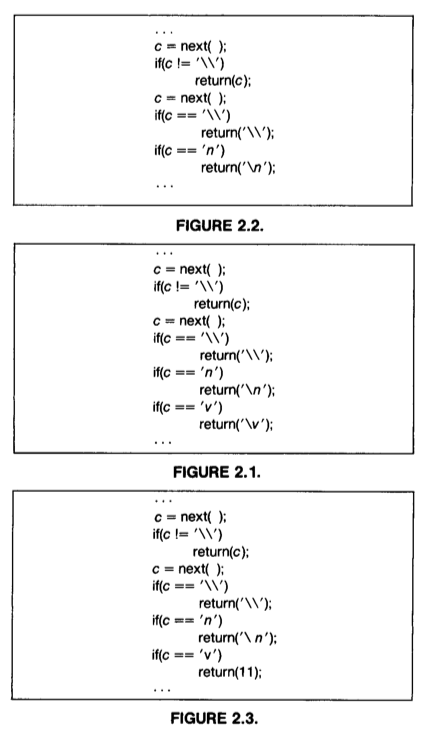
\includegraphics[width=0.8\linewidth]{img/image_2023-01-13-05-03-27.png}
    \caption{Teaching a compiler what the "\textbackslash v" sequence is. We may add a statement to return the ascii encoding of \textbackslash v (11), compile the compiler, and then use it to compile a program that knows what \textbackslash v is. }. We may then alter the source to be like Figure 2.3 without any mention of \textbackslash v but still compile programs with \textbackslash v just fine.
\end{figure}

\begin{figure}[H]
    \centering
    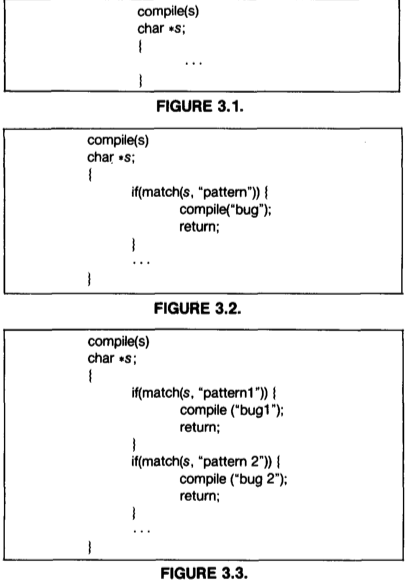
\includegraphics[width=0.8\linewidth]{img/image_2023-01-13-05-08-29.png}
\end{figure}

Next, consider the above scenario where we insert a login Trojan to insert backdoors into code matching the unix login function. We may then compile the $ c $ compiler to do just that, and then change the source to what it should look like without the Trojan. Compiling the compiler one more time will now produce a compiler binary that looks completely innocent but will reinsert the Trojan wherever it can.


The moral of the story is that you can't trust code that you didn't totally create yourself. But it's awfully difficult to use only code written by oneself. So take security seriously.

\subsection{Software Code Vulnerabilities}


Recall: the stack is used to keep track of return addresses across function calls; storing a breadcrumb trail.
Another key thing sitting in the stack are local variables. 
A common theme in the course is that computing tends to conflate execution instructions with data.

Common data formats and structures create an opportunity for things to get confused (and for attackers to take advantage of). 
For example, a buffer-overflow attack can end up overwriting that return address breadcrumb trail and then execute arbitrary code.

\begin{figure}[H]
    \centering
    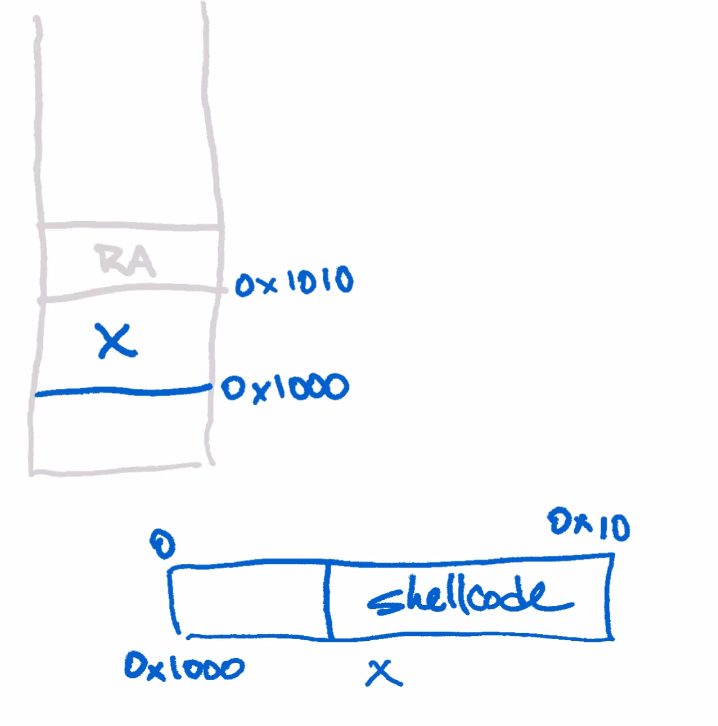
\includegraphics[width=0.8\linewidth]{img/image_2023-01-16-18-27-59.png}
    \caption{Bufferoverflow to write to the return address. Shellcode is a sequence of instructions that is used as the payload of an attack. It si called a shellcode because they commonly are used to start a shell from which the attacker can do more.}
\end{figure}


There are ways to find out where that return address is (or at least reasonably guess).
This is discussed more in detail later; for now we'll assume that they have it figured out.


A common technique to make this easier is to inject a bunch of \texttt{NOP}s before the start of the shellcode. So that we don't need to be as precise as needed in order to find the shellcode start.

One technique for finding the RA would be to incrementally increase the size of the buffer overflow until we get a segfault -- at this point the segfault would tell you what memory address it was trying to access and possibly the values it saw there instead as well.

\begin{figure}[H]
    \centering
    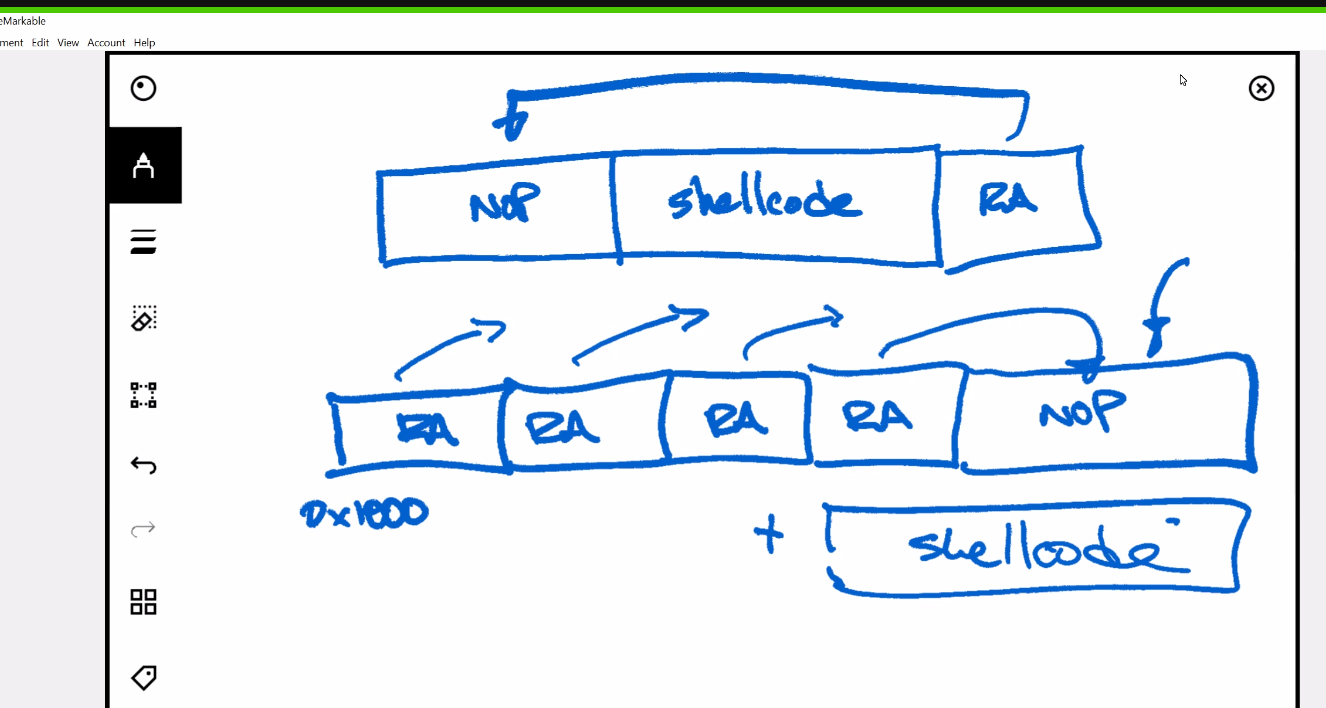
\includegraphics[width=0.8\linewidth]{img/image_2023-01-16-18-37-29.png}
    \caption{Can create a RA sled with a NOP leading to shellcode and then try it from e.g. 0x1000, 0x2000 and so forth to find where to attack from.}



\end{figure}

\begin{figure}[H]
    \centering
    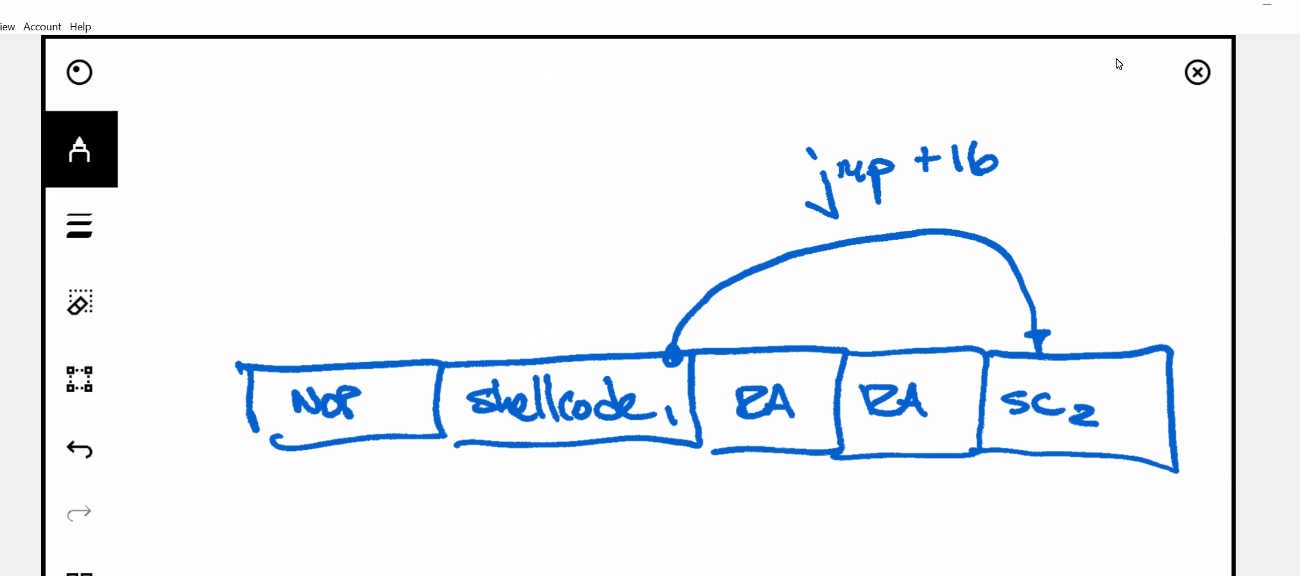
\includegraphics[width=0.8\linewidth]{img/image_2023-01-16-18-40-09.png}
    \caption{Another technique may involve placing shellcode all over the place, of which each one may be a valid entrypoint into the shellcode.}
\end{figure}



\subsection{Format string Vulnerabilities}
\begin{listing}[H]
\begin{minted}{c}
spirntf(buf, "Hello %s", name);
\end{minted}
\end{listing}


\texttt{sprint} is similar to \texttt{printf} except the output is copied into \texttt{buf}. The vulnerability is simiar to the buffer overflow vulnerability. The difference is that the attacker can control the format string.

Consider the following:

\begin{listing}[H]
\begin{minted}{c}
char* str = "Hello world";
printf(str); // 1
printf("%s", str); // 2
\end{minted}
\end{listing}

Despite it looking different there are differences in these two ways to print hello world.
The first argument is a format string, which is different from just a parameter.
A format string contains both instructions for the \texttt{c} printing library as well as data.
This means that the first method can be exploited if the attacker has access to the format string.
A more complex vulnerability is with \texttt{snprintf} (which limits the number of characters written into buf).



\begin{listing}[H]
\begin{minted}{c}
void main() {
    const int len = 10;
    char buf[len];
    snprintf(buf, len, "AB%d%d", 5, 6);
    // buf is now "AB56"
}
\end{minted}
\end{listing}

\begin{itemize}
    \item Arguments are pushed to the stack in reverse order
    \item snprintf copies data from the format string until it reaches a \%. The next argument is then fetched and outputted in the requested format
    \item What happens if there are more \% parameters than arguments? The argument pointer keeps moving up the stack and then points to values in the previous frame (and could actually look at your entire program memory, really)
\end{itemize}

\begin{listing}[H]
\begin{minted}{c}
void main () {
    char buf[256];
    snprintf(buf, 256, "AB,%08x,%08x,%08x,%08x,%08x,%08x,%08x,%08x,%08x,%08x", 5);
    printf(buf);
    // AB,00000005,00000000,29ee6890,302c4241,2c353030,30303030,
    // 39383665,32346332,33353363,30333033
    // if we look at the 3rd clause as ascii we get '0,BA'
   //  (recall intel little endian) i.e. we've read up far enough to see the local variable
   // specifying the format string pushed onto the stack earlier
}
\end{minted}
\end{listing}
\begin{figure}[H]
    \centering
    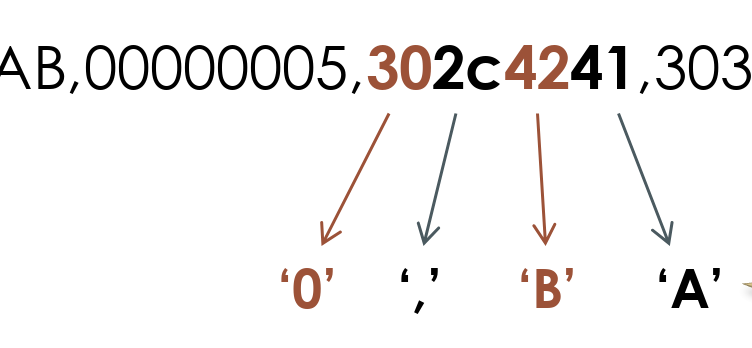
\includegraphics[width=0.8\linewidth]{img/image_2023-01-16-19-06-48.png}
    \caption{ASCII decoding}
\end{figure}

Now there's a potential problem: information leakage (of important info further up the stack).
Programmers may not pay attention to sanitizing input like language config.


\begin{itemize}
    \item \texttt{\%n}: Assume then next argument is a pointer and then it writes the number of characters printed so far into that pointer. 
    \item This can be abused by \%n  write to the return address and then overwrite it with the address of the shellcode.
\end{itemize}


How an exploit may look like for this is as follows:

\begin{figure}[H]
    \centering
    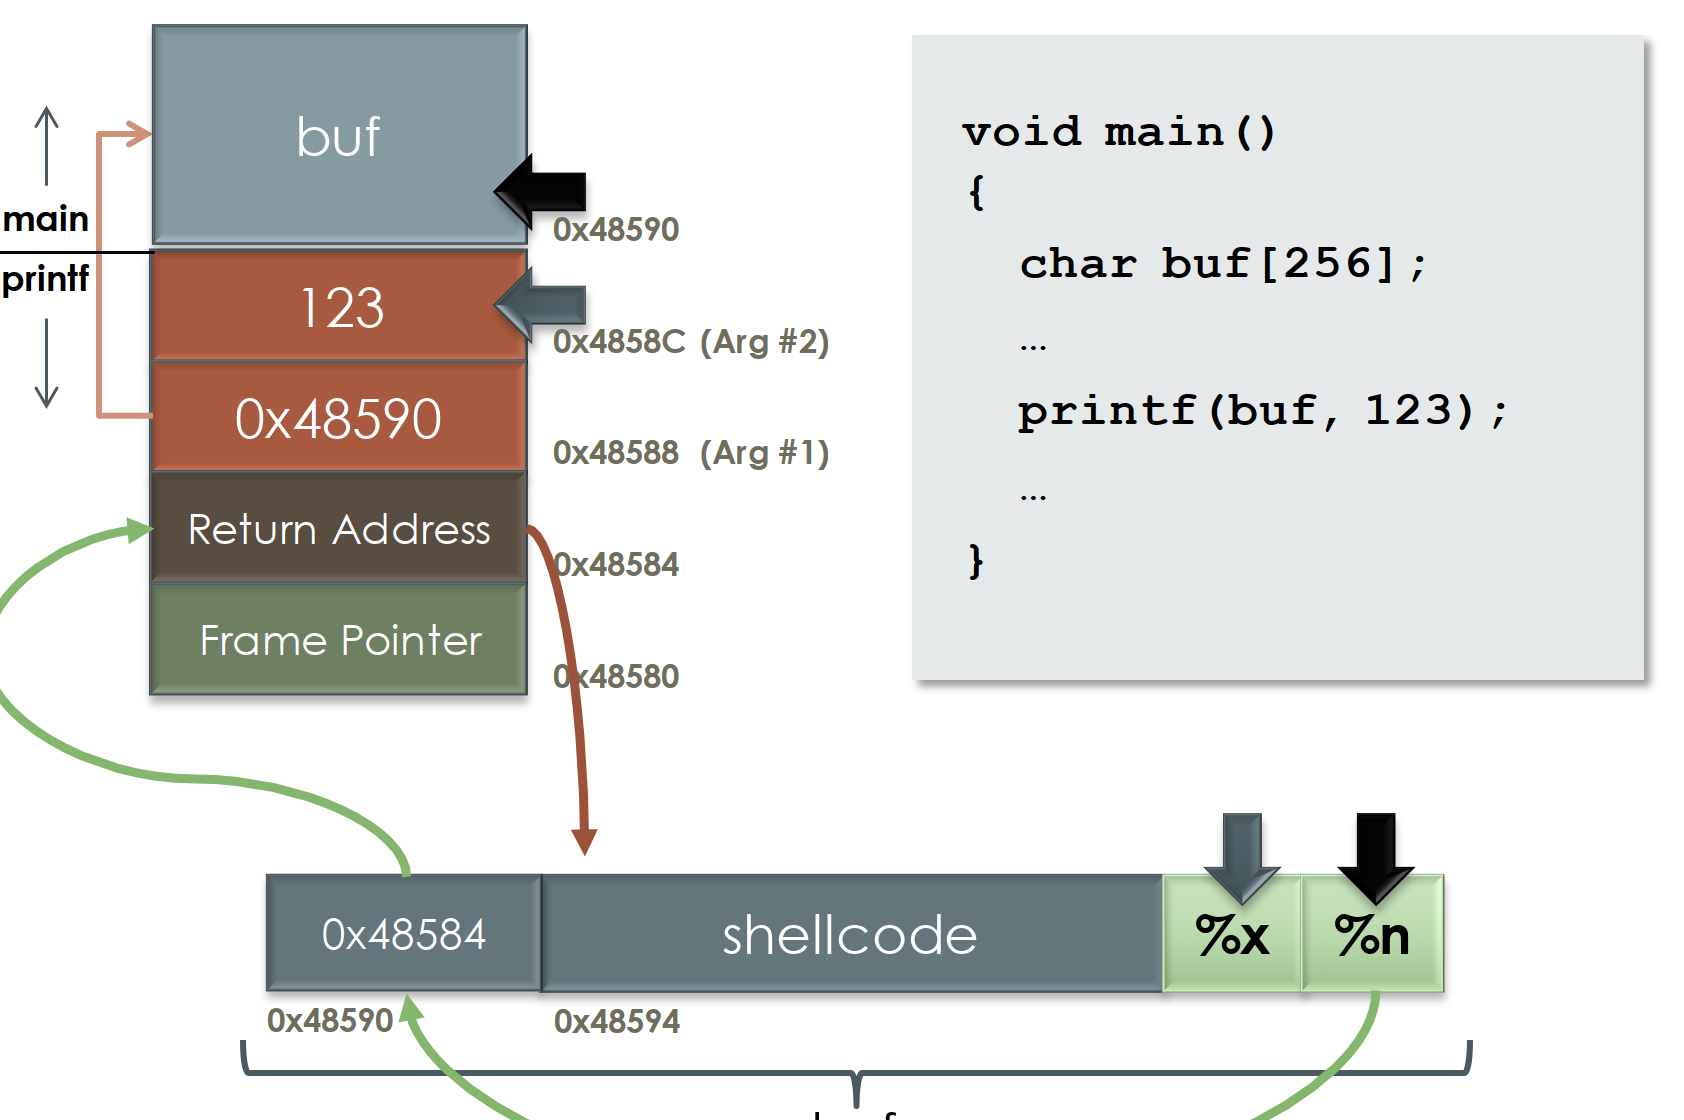
\includegraphics[width=0.8\linewidth]{img/image_2023-01-16-19-39-16.png}
\end{figure}

\begin{enumerate}
    \item Consume the 123 argument (\%x)
    \item Have the return address sitting in the beginning of the memory
    \item Overwrite the RA value with the start of shellcode
\end{enumerate}

There are some problems with this because on modern machines addresses are very large and it can be impractical to create a gigabyte-sized buffer.
Instead we can just divide the problem up and write multiple 8 bit numbers

\begin{figure}[H]
    \centering
    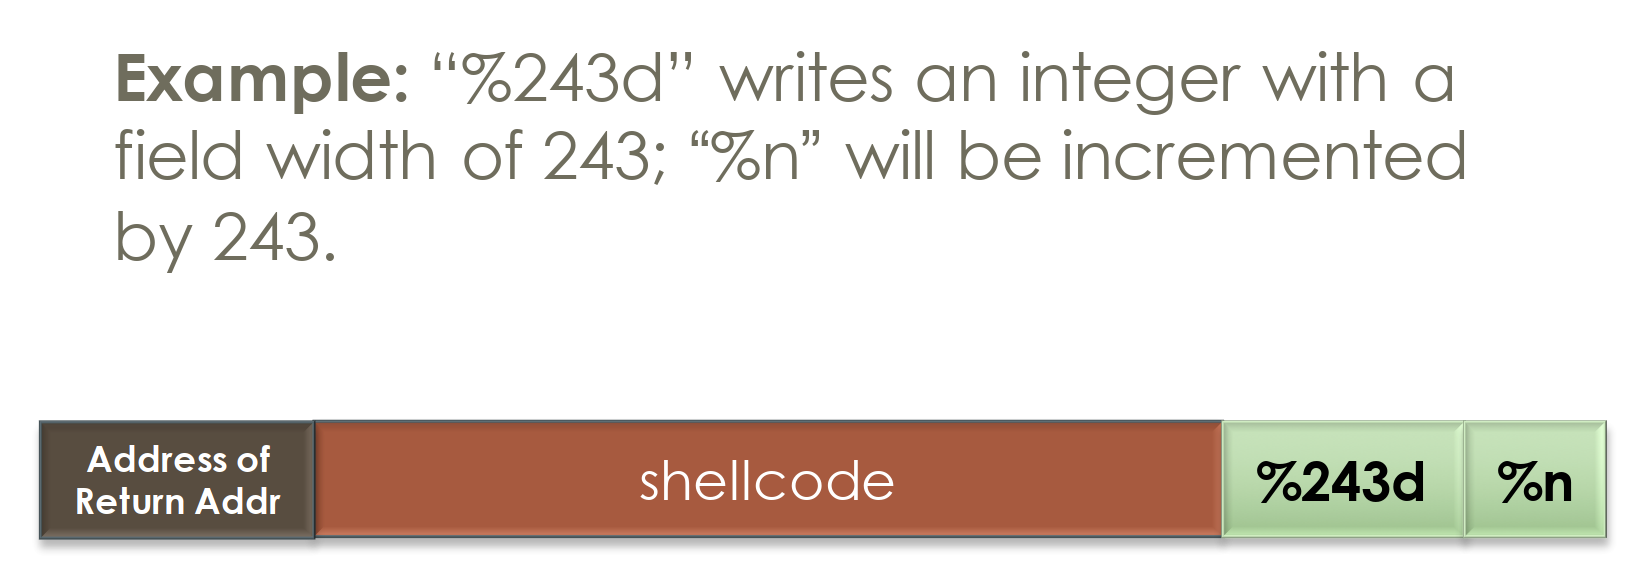
\includegraphics[width=0.8\linewidth]{img/image_2023-01-16-19-46-14.png}
    \caption{The printf count increments by 243 with \%243d. Shorthand}
\end{figure}


\begin{figure}[H]
    \centering
    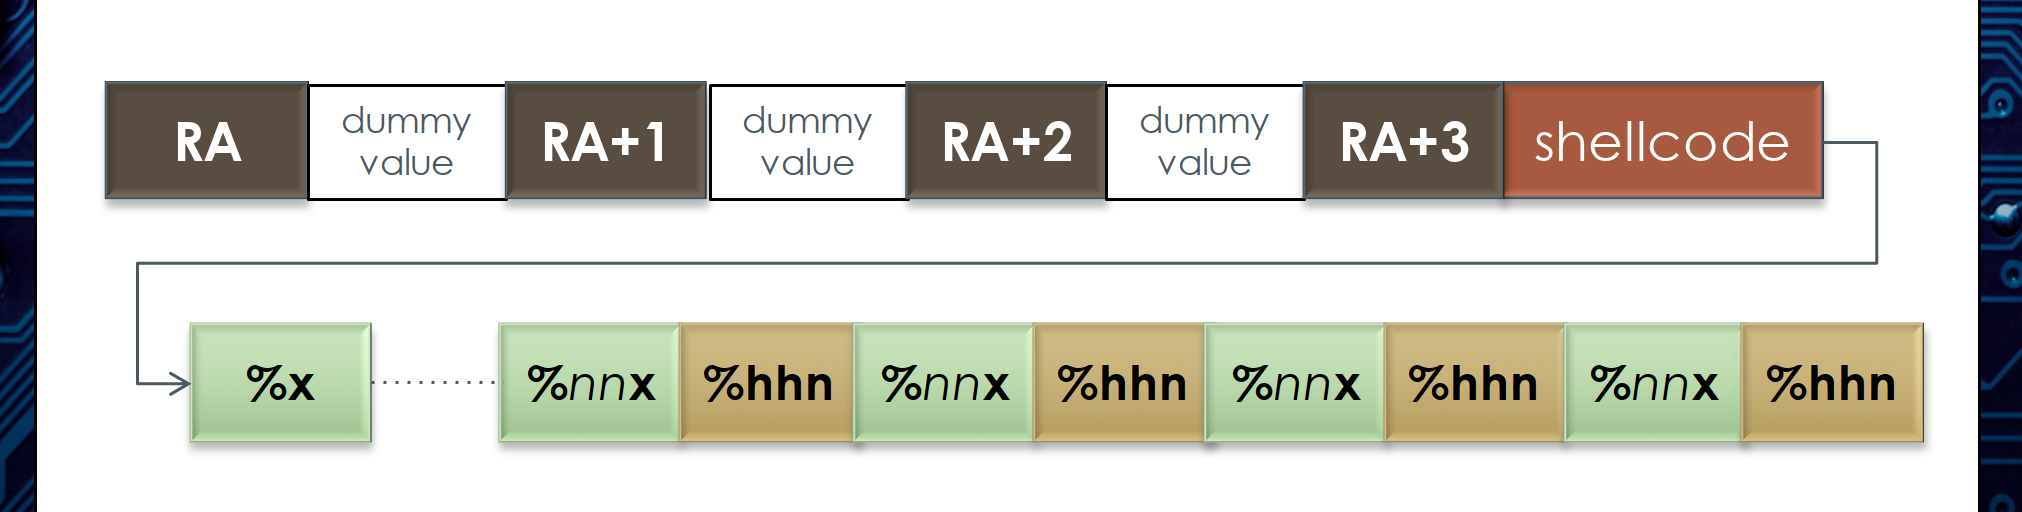
\includegraphics[width=0.8\linewidth]{img/image_2023-01-16-19-48-17.png}
    \caption{The gaps are there because }
\end{figure}
Dividing the problem into pieces; using \%hhn and \%nnx to write 8 bits at a time. \marginnote{Note that this writes the printf counter into the pointer at the argument. This drastically decreases the buffer size needed}

If the bytes being written must be written in decreasing order we can do this by structuring our pointers in a way that we write it in reverse order (don't need to start with LSB). Another option is 



\subsection{Double-Free vulnerability}

Freeing a memory location that is under the control of an attacker is an exploitable vulnerability


\begin{listing}[H]
\begin{minted}{c}
p = malloc(128);
q = malloc(128);
free(p);
free (q);
p = malloc(256);
// this is where the attack happens; the fake tag, shell code, etc
strcpy(p, attacker_string);
free(q);
\end{minted}
\end{listing}

Note that the \texttt{c} free function takes a reference (not necessarily a pointer) to the memory location to be freed. It does not change the value of the free'd pointer either.

\begin{figure}[H]
    \centering
    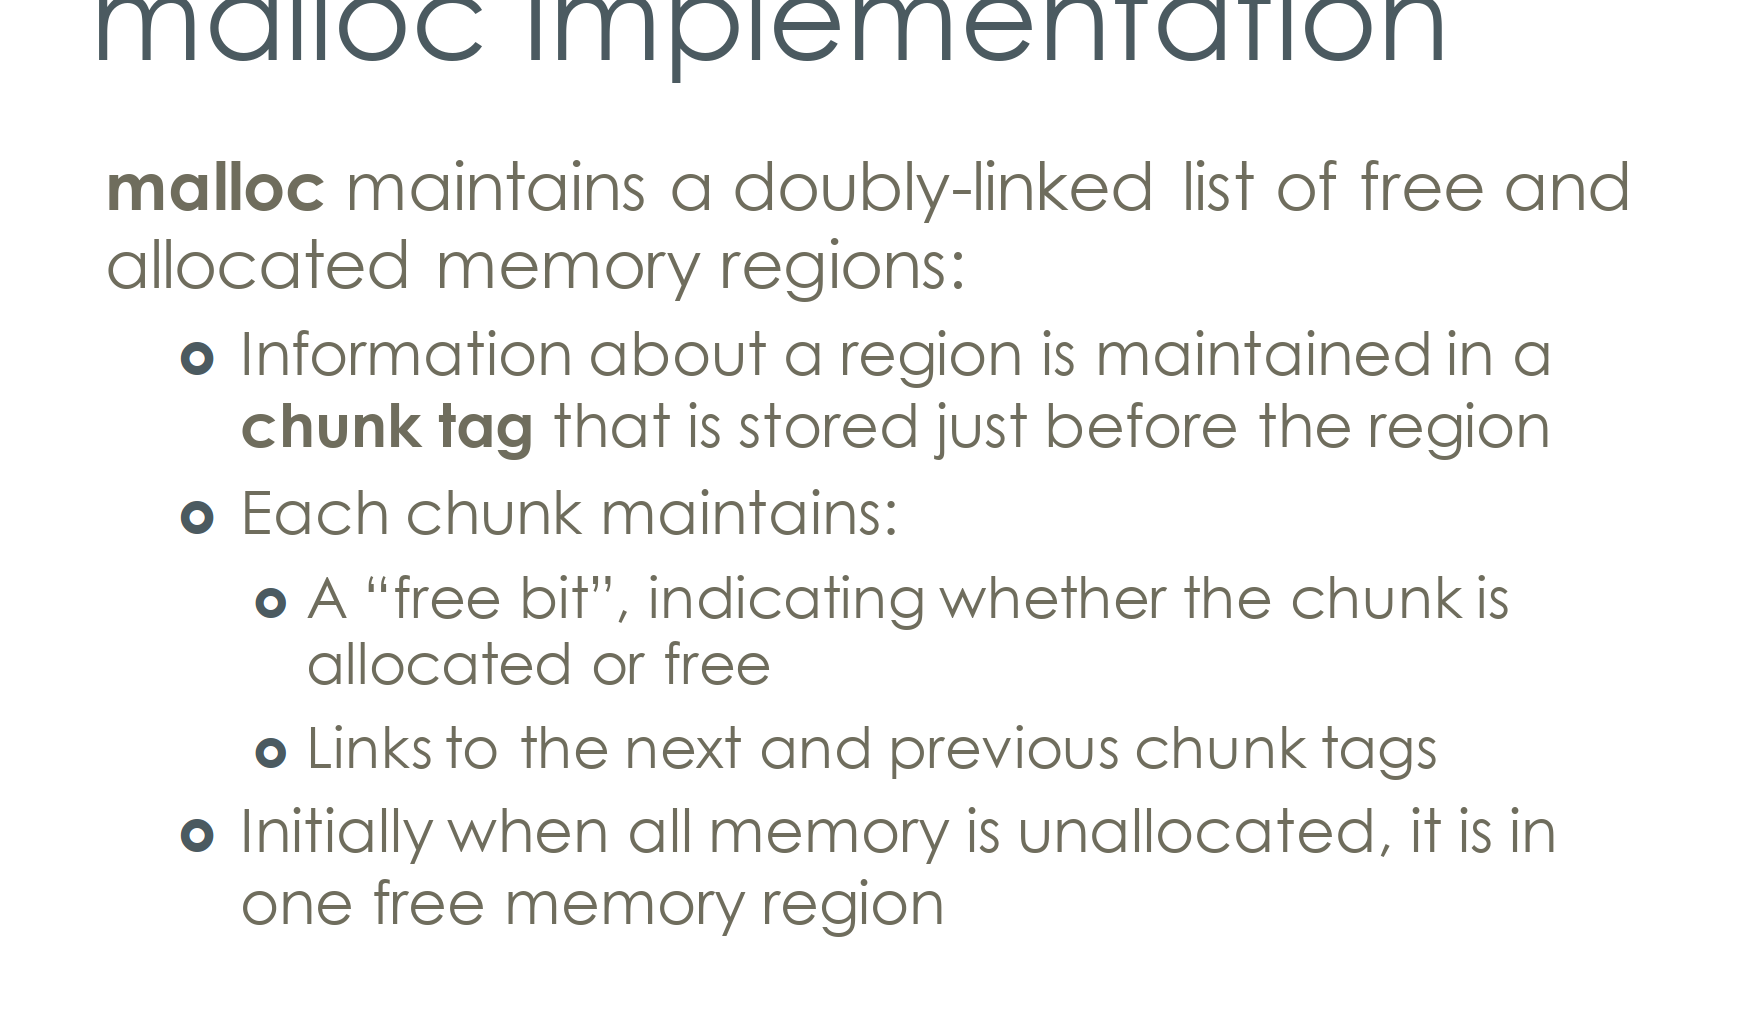
\includegraphics[width=0.8\linewidth]{img/image_2023-01-16-20-08-50.png}
\end{figure}

\begin{figure}[H]
    \centering
    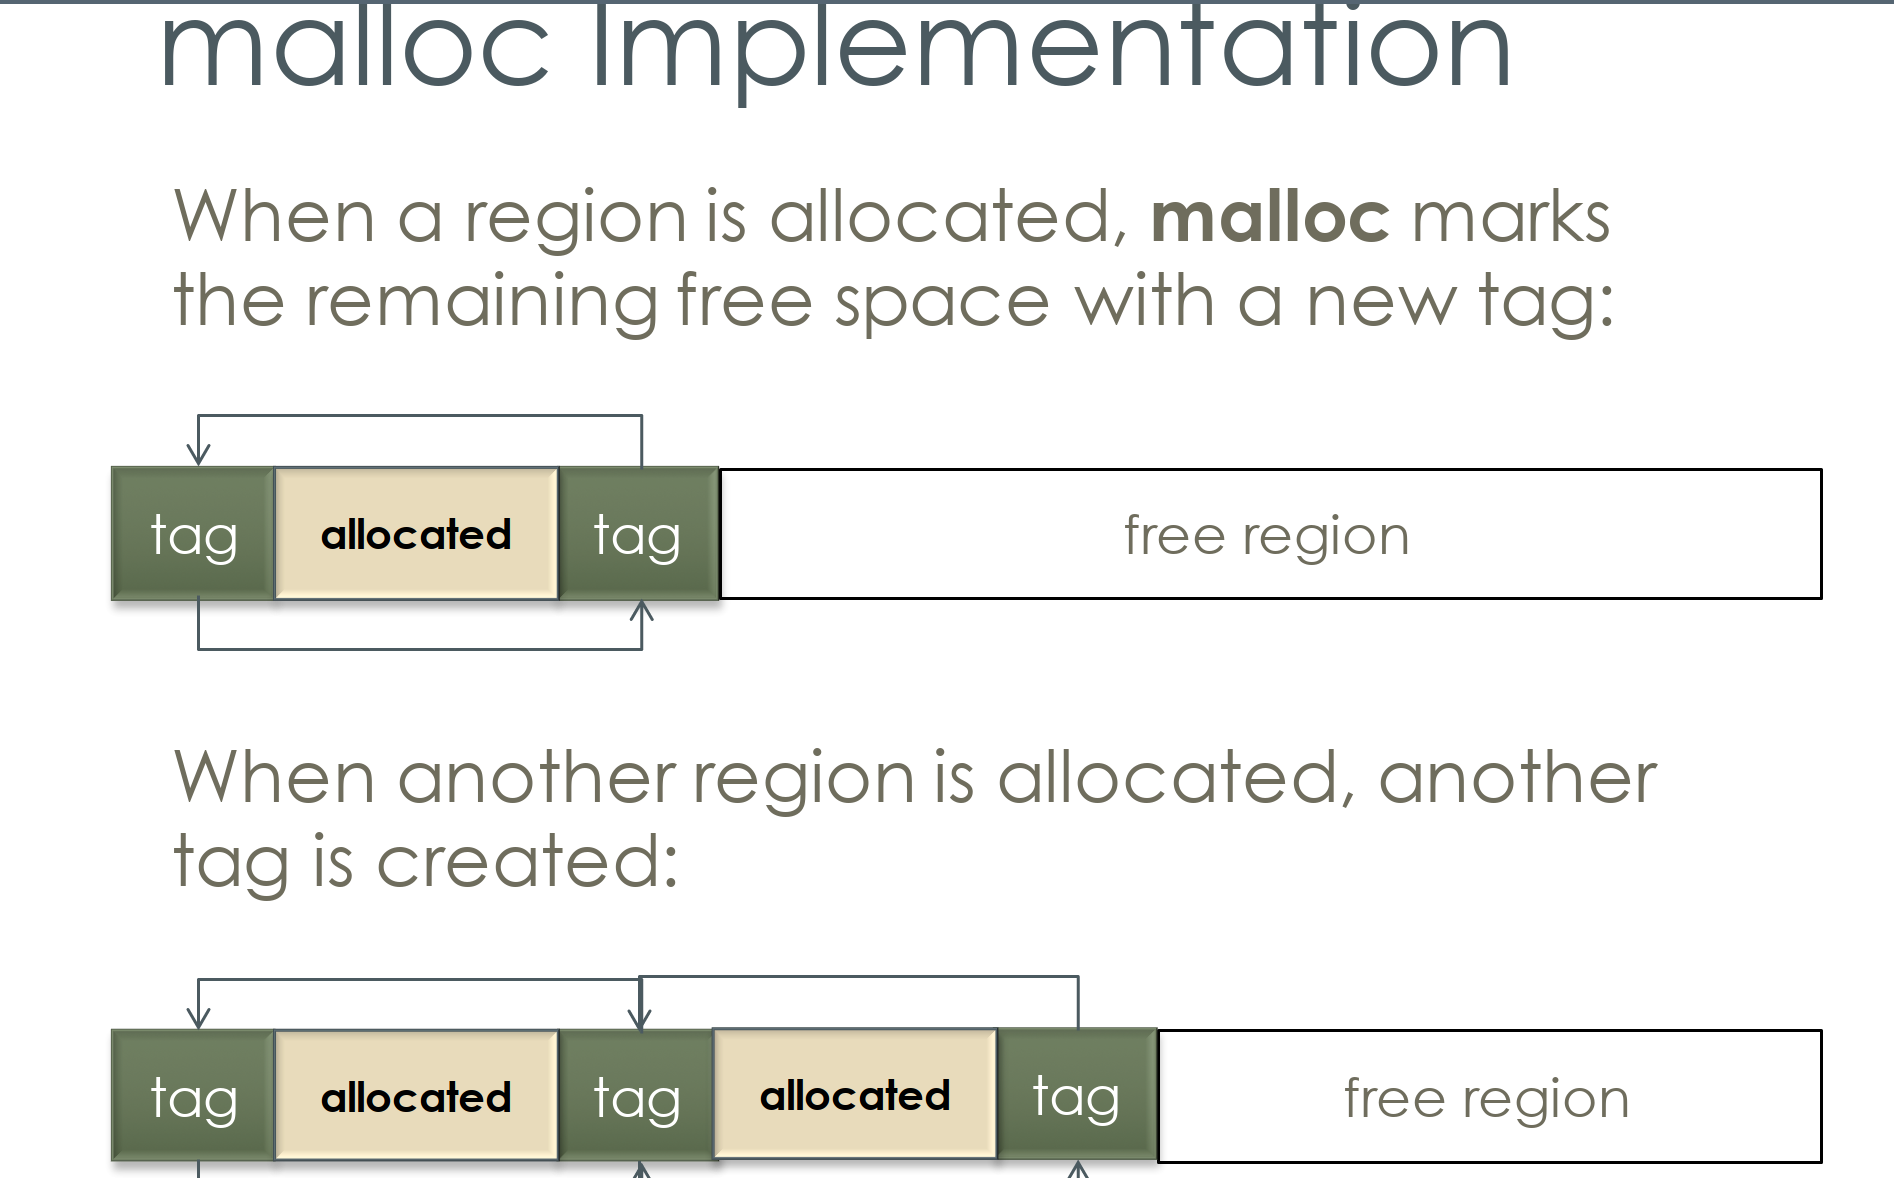
\includegraphics[width=0.8\linewidth]{img/image_2023-01-16-20-09-02.png}
\end{figure}

Malloc places a doubly-linked-list of chunk bits in memory to describe the memory allocated. \texttt{free} sets the free bit, does the various doubly linked list operations (looking at the pointer values of its neighbours in order to remove itself) and also tries to consolidate adjacent free regions.
It assumes that it is passed the beginning of the allocated memory as well as go find the tag associated with the region (which is in a consistent place every time).

The attacker can drop fake tags into memory just ahead of the value we want to overwrite and then we can use the free() call to overwrite memory with the attacker's data.
For example we can create a fake tag node with a prev and next pointer. We make the next pointer be the address of the return address. And then "prev" can contain the address of the start of our shellcode. So freeing on this fake tag will overwrite the return address with the shellcode start.



\begin{blockquote}
    Note that this is not possible with a single free if you are not able to write to negative memory indicies. 
    The part that makes this attack works is that the double free allows the attacker to write a fake tag just before the next tag in a totally valid way. Doing this with a single free would also involve writing to memory that the program doesn't own. (recall: how the memory manager works)
    

\end{blockquote}





\subsection{Other common vulnerabilities}

The attacks we have seen have involved overwriting the return address to point to injecting code. Are there ways to exploit software without injecting code? Yes -- return into \texttt{libc} i.e. use \texttt{libc}'s \texttt{system} library call which looks already like shell code.
This can be accomplished with any of the exploits we have already talked about.

I.e.

\begin{itemize}
    \item Change the return addresses to point to start of the system function
    \item Inject a stack frame on the stack
    \item Before return sp points to $ \&system $
    \item System looks in stack for arguments
    \item System executes the command, i.e maybe a shell
\end{itemize}


\begin{itemize}
    \item Function pointers
    \item Dynamic linking
    \item Integer overflows
    \item Bad bounds checking
\end{itemize}


\subsubsection{Attacks without overwriting the return address}

Finding return addresses is hard. So we can use other methods to inject code into the program.

\begin{itemize}
    \item Function pointers: an adversary can just try to overwrite a function pointer
    \item An area where this is very common is with \textit{dynamic linking}, i.e. functions such as \textit{printf}. 
    \item Typically both the caller of the library function and the function itself are compiled to be position independent
    \item We need to map the position independent function call to the absolute location of the function code in the library
    \item The dynamic linker performs this mapping with the procedure linkage table and the global offset table
        \begin{itemize}
            \item GOT is a table of pointers to functions; contains absolute mem location of each of the dyn-loaded library functions
            \item PLT is a table of code entries: onee per each library function called by program, i.e. sprintf@plt
            \item Similar to a switch statement
            \item Each code entry invoes the function pointer in the GOT
            \item i.e. sprintf@plt may invoke jmp GOT[k] where k is the index of sprintf in the GOT
            \item So if we change the pointers in the offset table we can make the program call our own code, i.e. with objdump.\mn{PLT/GOT always appears at a known location.}

        \end{itemize}
\end{itemize}




\subsubsection{Return-Oriented Programming}
\begin{itemize}
    \item An exploit that uses carefully-selected sequences of existing instructions located at the end of existing functions (gadgets) and then executes functions in an order such that these gadgets compose together to deliver an exploit. 
    \item This can be done faster by seeding the stack with a sequence of return addresses corresponding to the gadgets and in the order we want to run them in.
\end{itemize}



\subsection{Software Code Vulnerabilities}


Recall: the stack is used to keep track of return addresses across function calls; storing a breadcrumb trail.
Another key thing sitting in the stack are local variables. 
A common theme in the course is that computing tends to conflate execution instructions with data.

Common data formats and structures create an opportunity for things to get confused (and for attackers to take advantage of). 
For example, a buffer-overflow attack can end up overwriting that return address breadcrumb trail and then execute arbitrary code.

\begin{figure}[H]
    \centering
    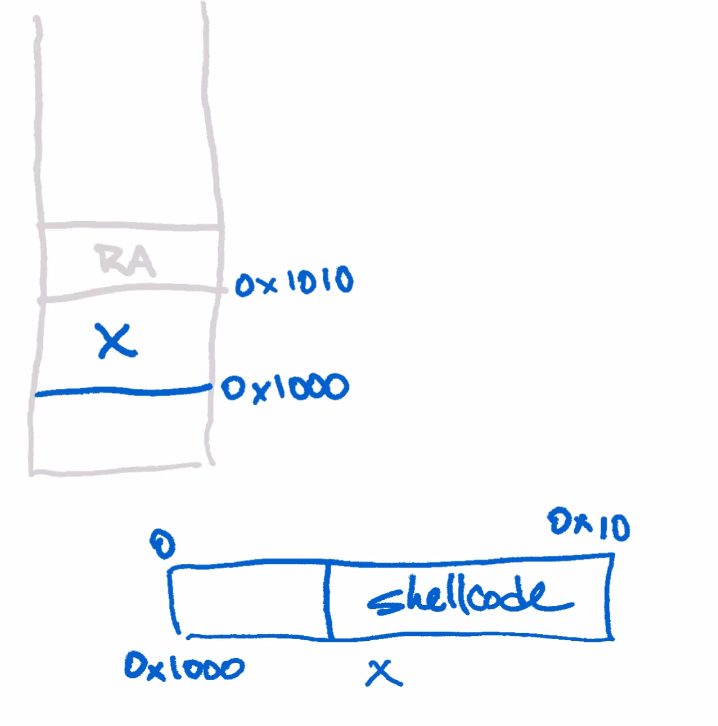
\includegraphics[width=0.8\linewidth]{img/image_2023-01-16-18-27-59.png}
    \caption{Bufferoverflow to write to the return address. Shellcode is a sequence of instructions that is used as the payload of an attack. It si called a shellcode because they commonly are used to start a shell from which the attacker can do more.}
\end{figure}


There are ways to find out where that return address is (or at least reasonably guess).
This is discussed more in detail later; for now we'll assume that they have it figured out.


A common technique to make this easier is to inject a bunch of \texttt{NOP}s before the start of the shellcode. So that we don't need to be as precise as needed in order to find the shellcode start.

One technique for finding the RA would be to incrementally increase the size of the buffer overflow until we get a segfault -- at this point the segfault would tell you what memory address it was trying to access and possibly the values it saw there instead as well.

\begin{figure}[H]
    \centering
    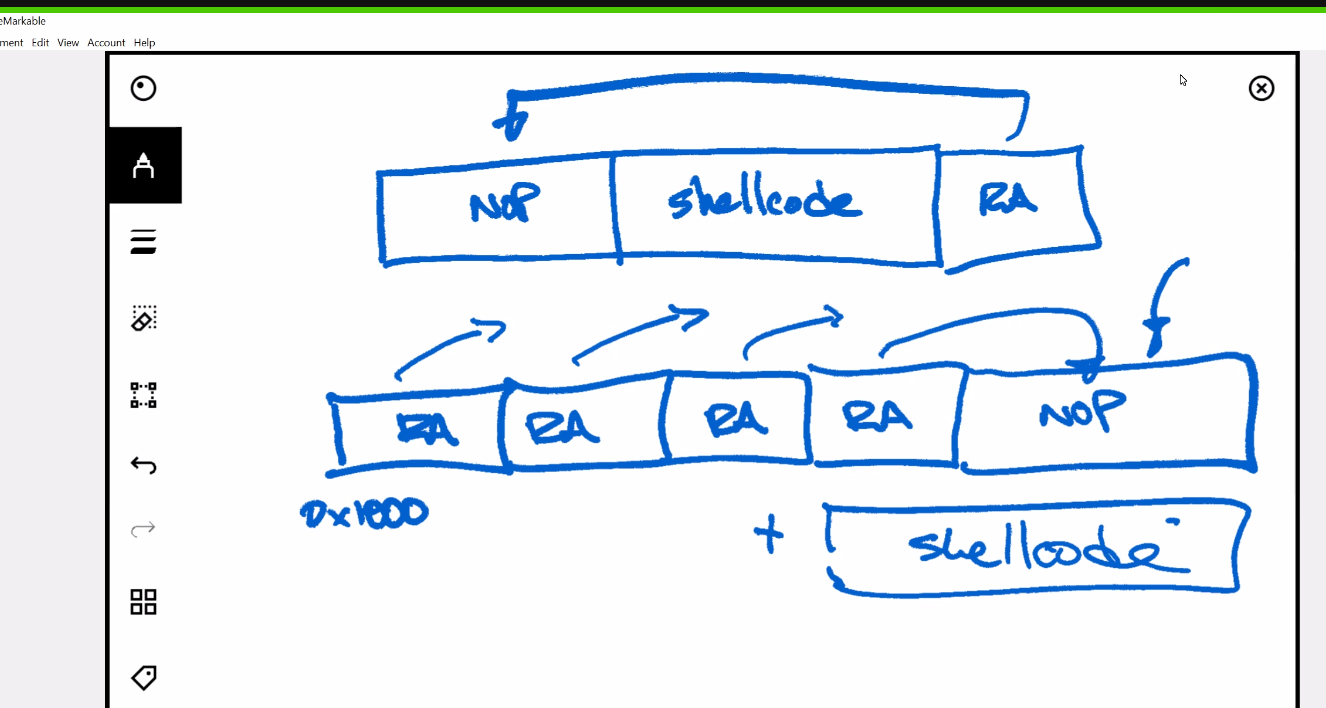
\includegraphics[width=0.8\linewidth]{img/image_2023-01-16-18-37-29.png}
    \caption{Can create a RA sled with a NOP leading to shellcode and then try it from e.g. 0x1000, 0x2000 and so forth to find where to attack from.}



\end{figure}

\begin{figure}[H]
    \centering
    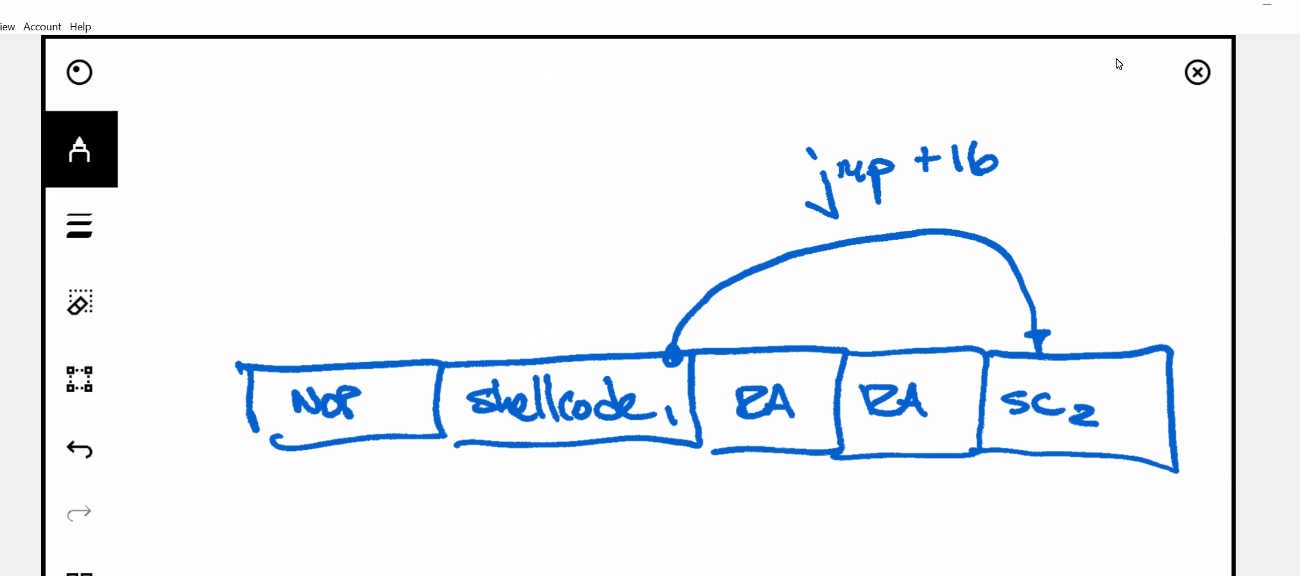
\includegraphics[width=0.8\linewidth]{img/image_2023-01-16-18-40-09.png}
    \caption{Another technique may involve placing shellcode all over the place, of which each one may be a valid entrypoint into the shellcode.}
\end{figure}



\subsection{Format string Vulnerabilities}
\begin{listing}[H]
\begin{minted}{c}
spirntf(buf, "Hello %s", name);
\end{minted}
\end{listing}


\texttt{sprint} is similar to \texttt{printf} except the output is copied into \texttt{buf}. The vulnerability is simiar to the buffer overflow vulnerability. The difference is that the attacker can control the format string.

Consider the following:

\begin{listing}[H]
\begin{minted}{c}
char* str = "Hello world";
printf(str); // 1
printf("%s", str); // 2
\end{minted}
\end{listing}

Despite it looking different there are differences in these two ways to print hello world.
The first argument is a format string, which is different from just a parameter.
A format string contains both instructions for the \texttt{c} printing library as well as data.
This means that the first method can be exploited if the attacker has access to the format string.
A more complex vulnerability is with \texttt{snprintf} (which limits the number of characters written into buf).



\begin{listing}[H]
\begin{minted}{c}
void main() {
    const int len = 10;
    char buf[len];
    snprintf(buf, len, "AB%d%d", 5, 6);
    // buf is now "AB56"
}
\end{minted}
\end{listing}

\begin{itemize}
    \item Arguments are pushed to the stack in reverse order
    \item snprintf copies data from the format string until it reaches a \%. The next argument is then fetched and outputted in the requested format
    \item What happens if there are more \% parameters than arguments? The argument pointer keeps moving up the stack and then points to values in the previous frame (and could actually look at your entire program memory, really)
\end{itemize}

\begin{listing}[H]
\begin{minted}{c}
void main () {
    char buf[256];
    snprintf(buf, 256, "AB,%08x,%08x,%08x,%08x,%08x,%08x,%08x,%08x,%08x,%08x", 5);
    printf(buf);
    // AB,00000005,00000000,29ee6890,302c4241,2c353030,30303030,39383665,
    // 32346332,33353363,30333033
    // if we look at the 3rd clause as ascii we get '0,BA' (recall intel little endian) i.e. we've read up far enough to see the local variable specifying the format string pushed onto the stack earlier
}
\end{minted}
\end{listing}
\begin{figure}[H]
    \centering
    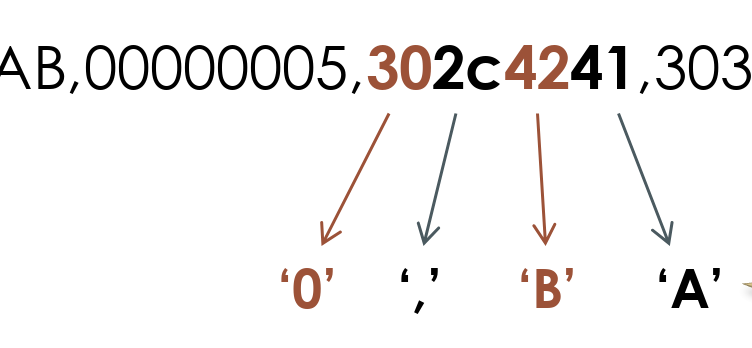
\includegraphics[width=0.8\linewidth]{img/image_2023-01-16-19-06-48.png}
    \caption{ASCII decoding}
\end{figure}

Now there's a potential problem: information leakage (of important info further up the stack).
Programmers may not pay attention to sanitizing input like language config.


\begin{itemize}
    \item \texttt{\%n}: Assume then next argument is a pointer and then it writes the number of characters printed so far into that pointer. 
    \item This can be abused by \%n  write to the return address and then overwrite it with the address of the shellcode.
\end{itemize}


How an exploit may look like for this is as follows:

\begin{figure}[H]
    \centering
    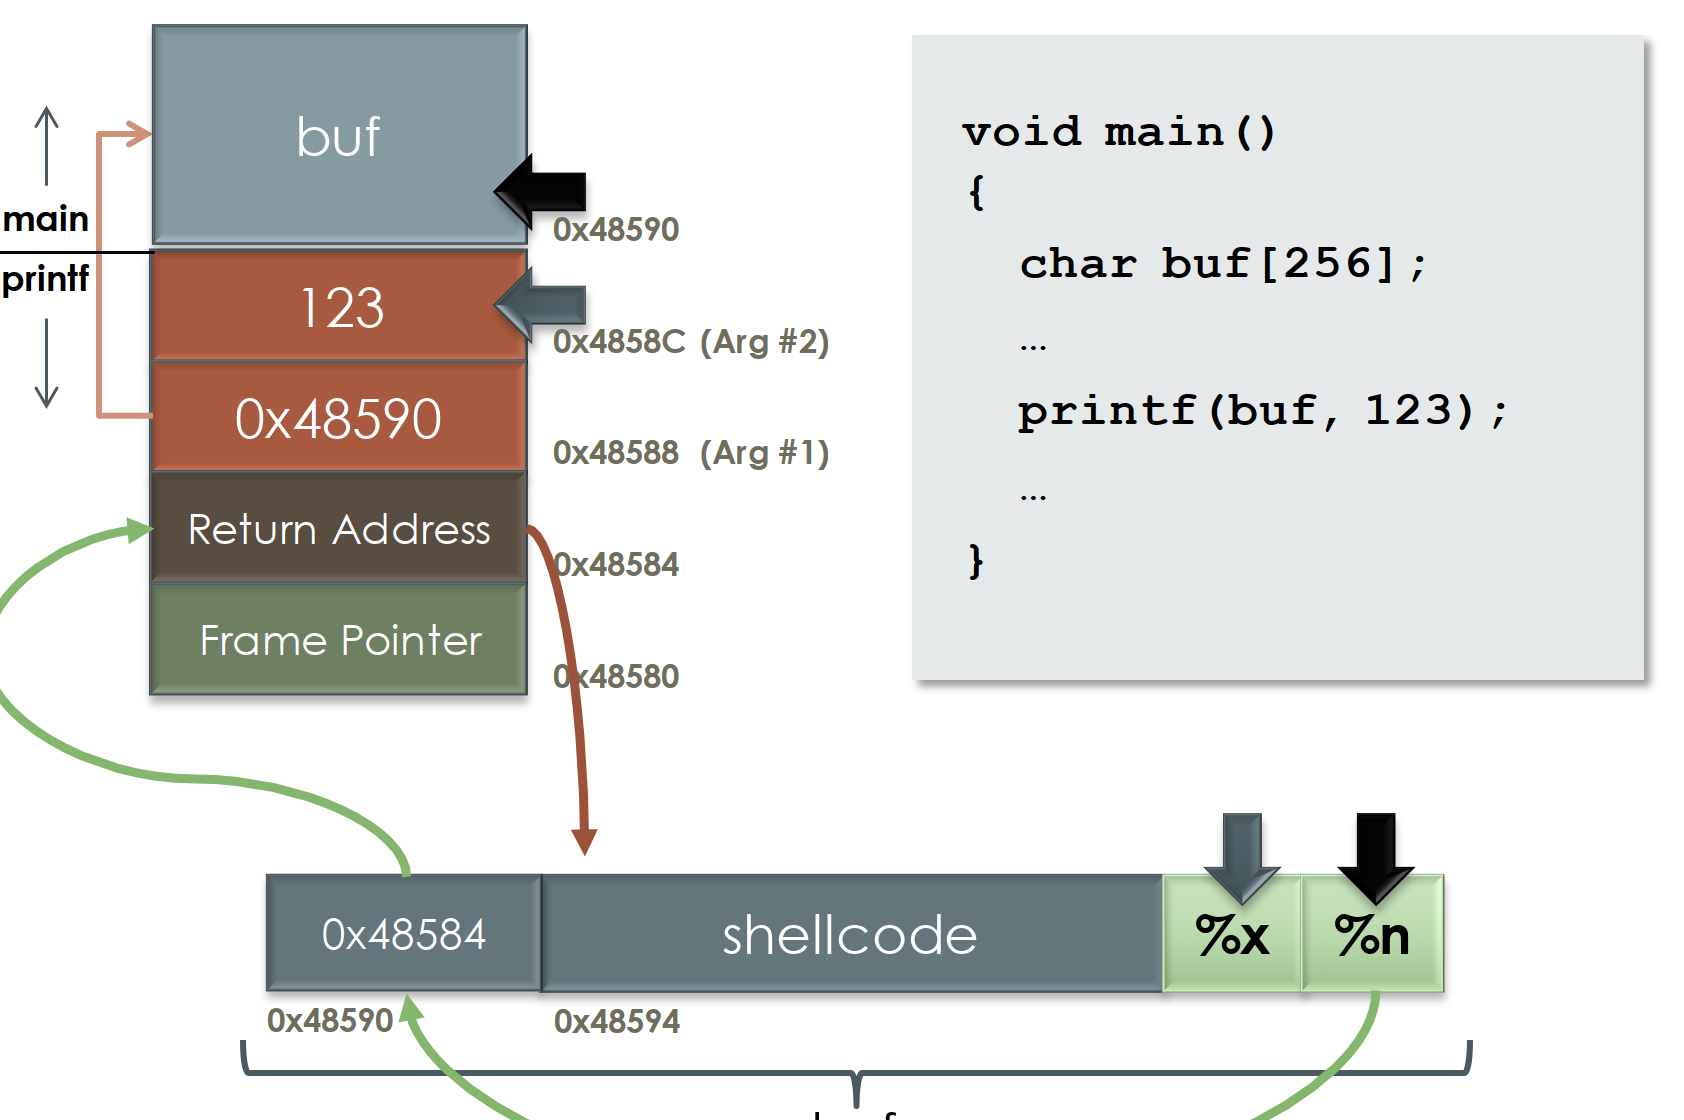
\includegraphics[width=0.8\linewidth]{img/image_2023-01-16-19-39-16.png}
\end{figure}

\begin{enumerate}
    \item Consume the 123 argument (\%x)
    \item Have the return address sitting in the beginning of the memory
    \item Overwrite the RA value with the start of shellcode
\end{enumerate}

There are some problems with this because on modern machines addresses are very large and it can be impractical to create a gigabyte-sized buffer.
Instead we can just divide the problem up and write multiple 8 bit numbers

\begin{figure}[H]
    \centering
    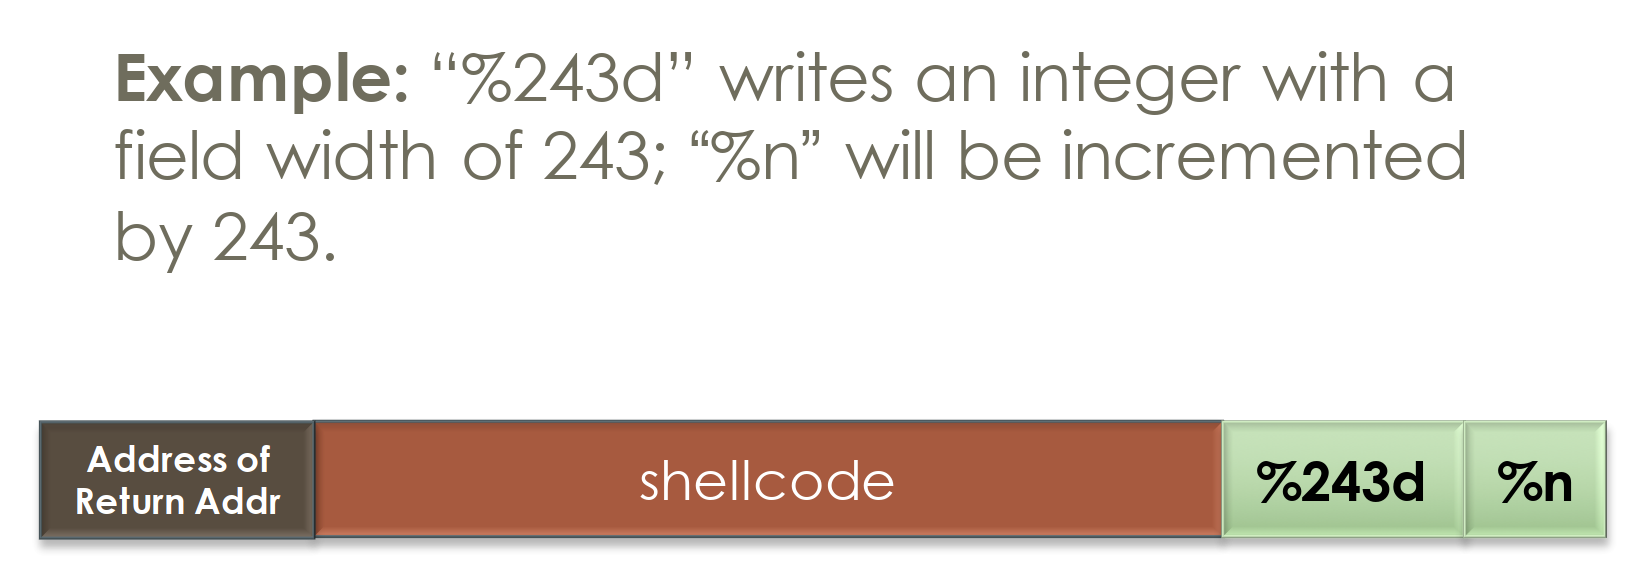
\includegraphics[width=0.8\linewidth]{img/image_2023-01-16-19-46-14.png}
    \caption{The printf count increments by 243 with \%243d. Shorthand}
\end{figure}


\begin{figure}[H]
    \centering
    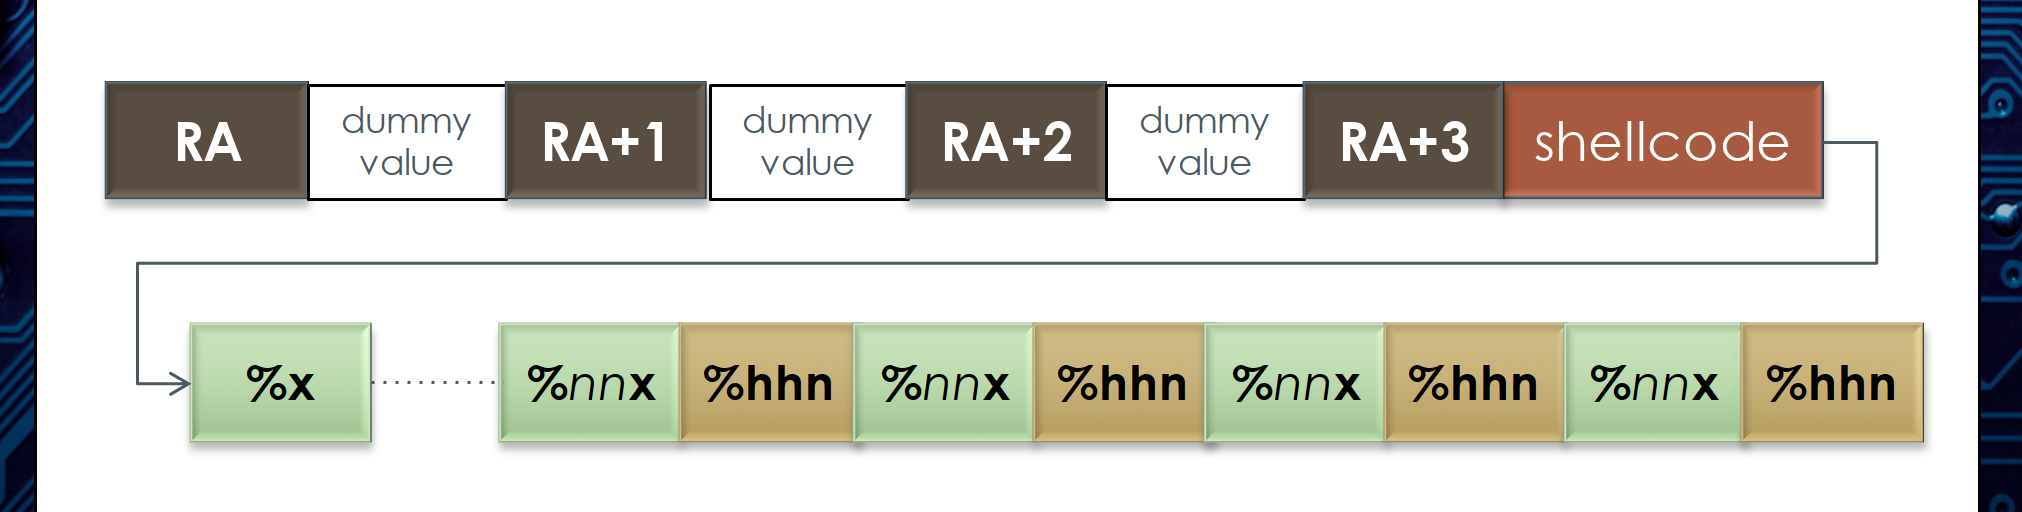
\includegraphics[width=0.8\linewidth]{img/image_2023-01-16-19-48-17.png}
    \caption{The gaps are there because }
\end{figure}
Dividing the problem into pieces; using \%hhn and \%nnx to write 8 bits at a time. \marginnote{Note that this writes the printf counter into the pointer at the argument. This drastically decreases the buffer size needed}

If the bytes being written must be written in decreasing order we can do this by structuring our pointers in a way that we write it in reverse order (don't need to start with LSB). Another option is 



\subsection{Double-Free vulnerability}

Freeing a memory location that is under the control of an attacker is an exploitable vulnerability


\begin{listing}[H]
\begin{minted}{c}
p = malloc(128);
q = malloc(128);
free(p);
free (q);
p = malloc(256);
// this is where the attack happens; the fake tag, shell code, etc
strcpy(p, attacker_string);
free(q);
\end{minted}
\end{listing}

Note that the \texttt{c} free function takes a reference (not necessarily a pointer) to the memory location to be freed. It does not change the value of the free'd pointer either.

\begin{figure}[H]
    \centering
    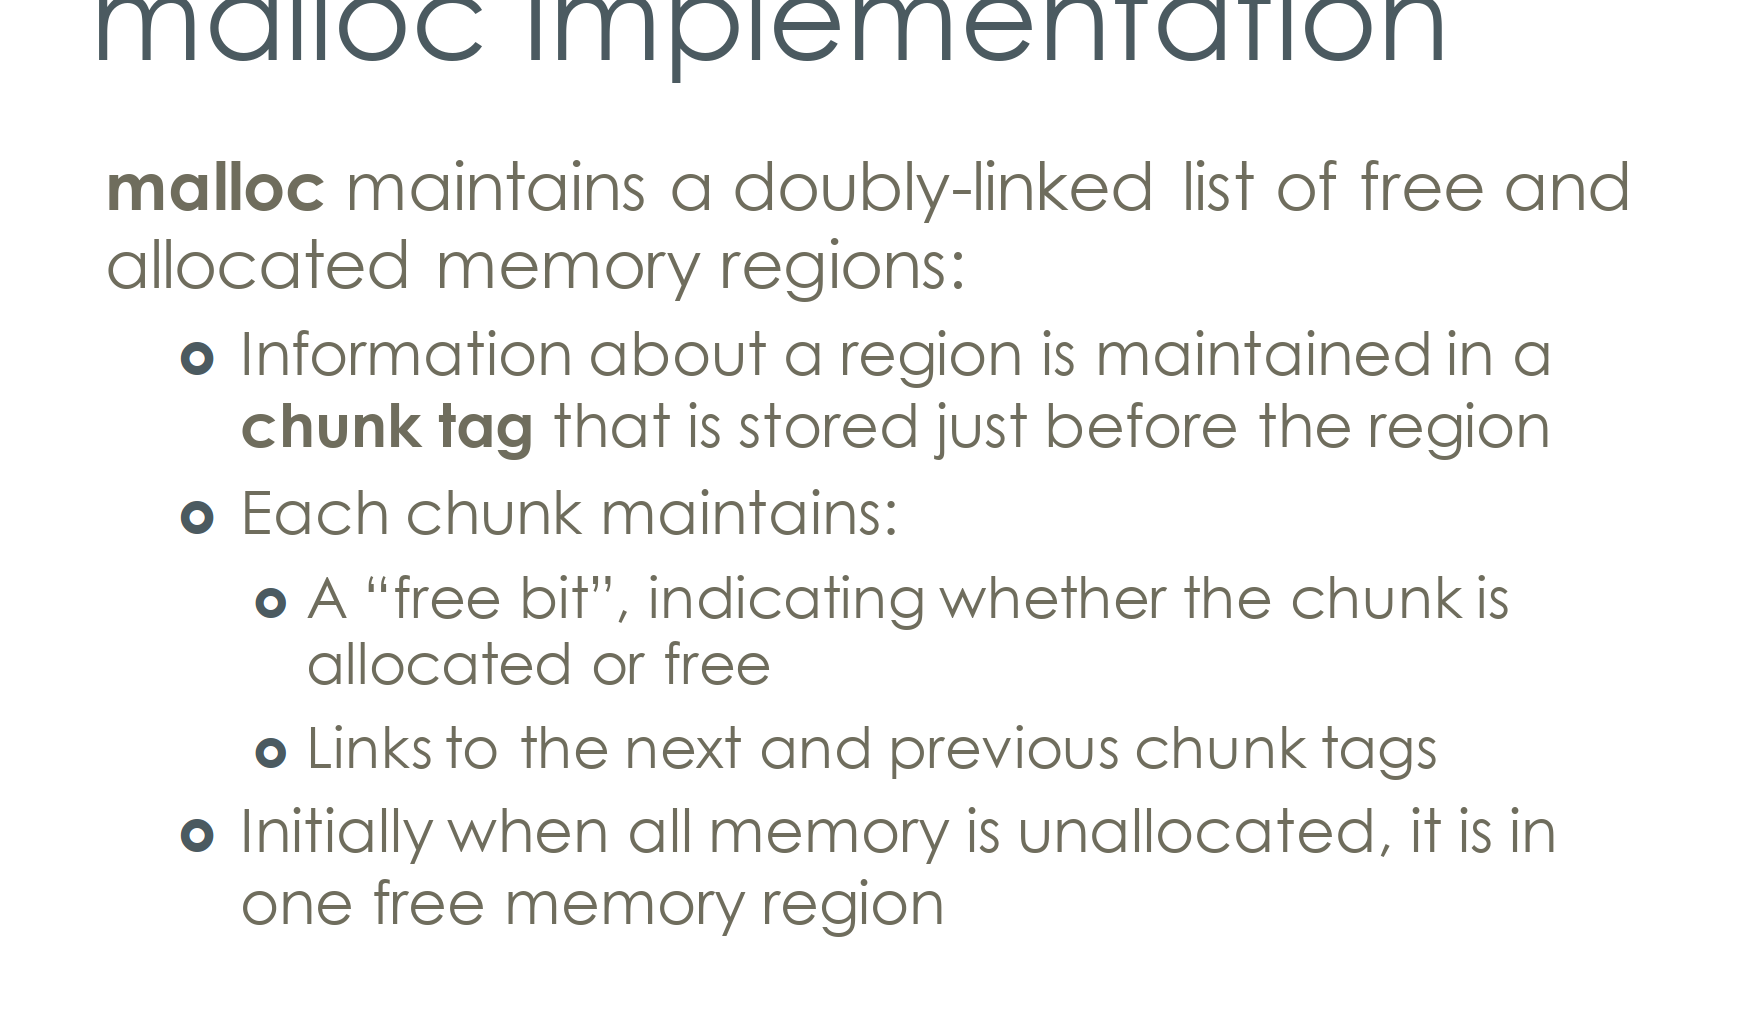
\includegraphics[width=0.8\linewidth]{img/image_2023-01-16-20-08-50.png}
\end{figure}

\begin{figure}[H]
    \centering
    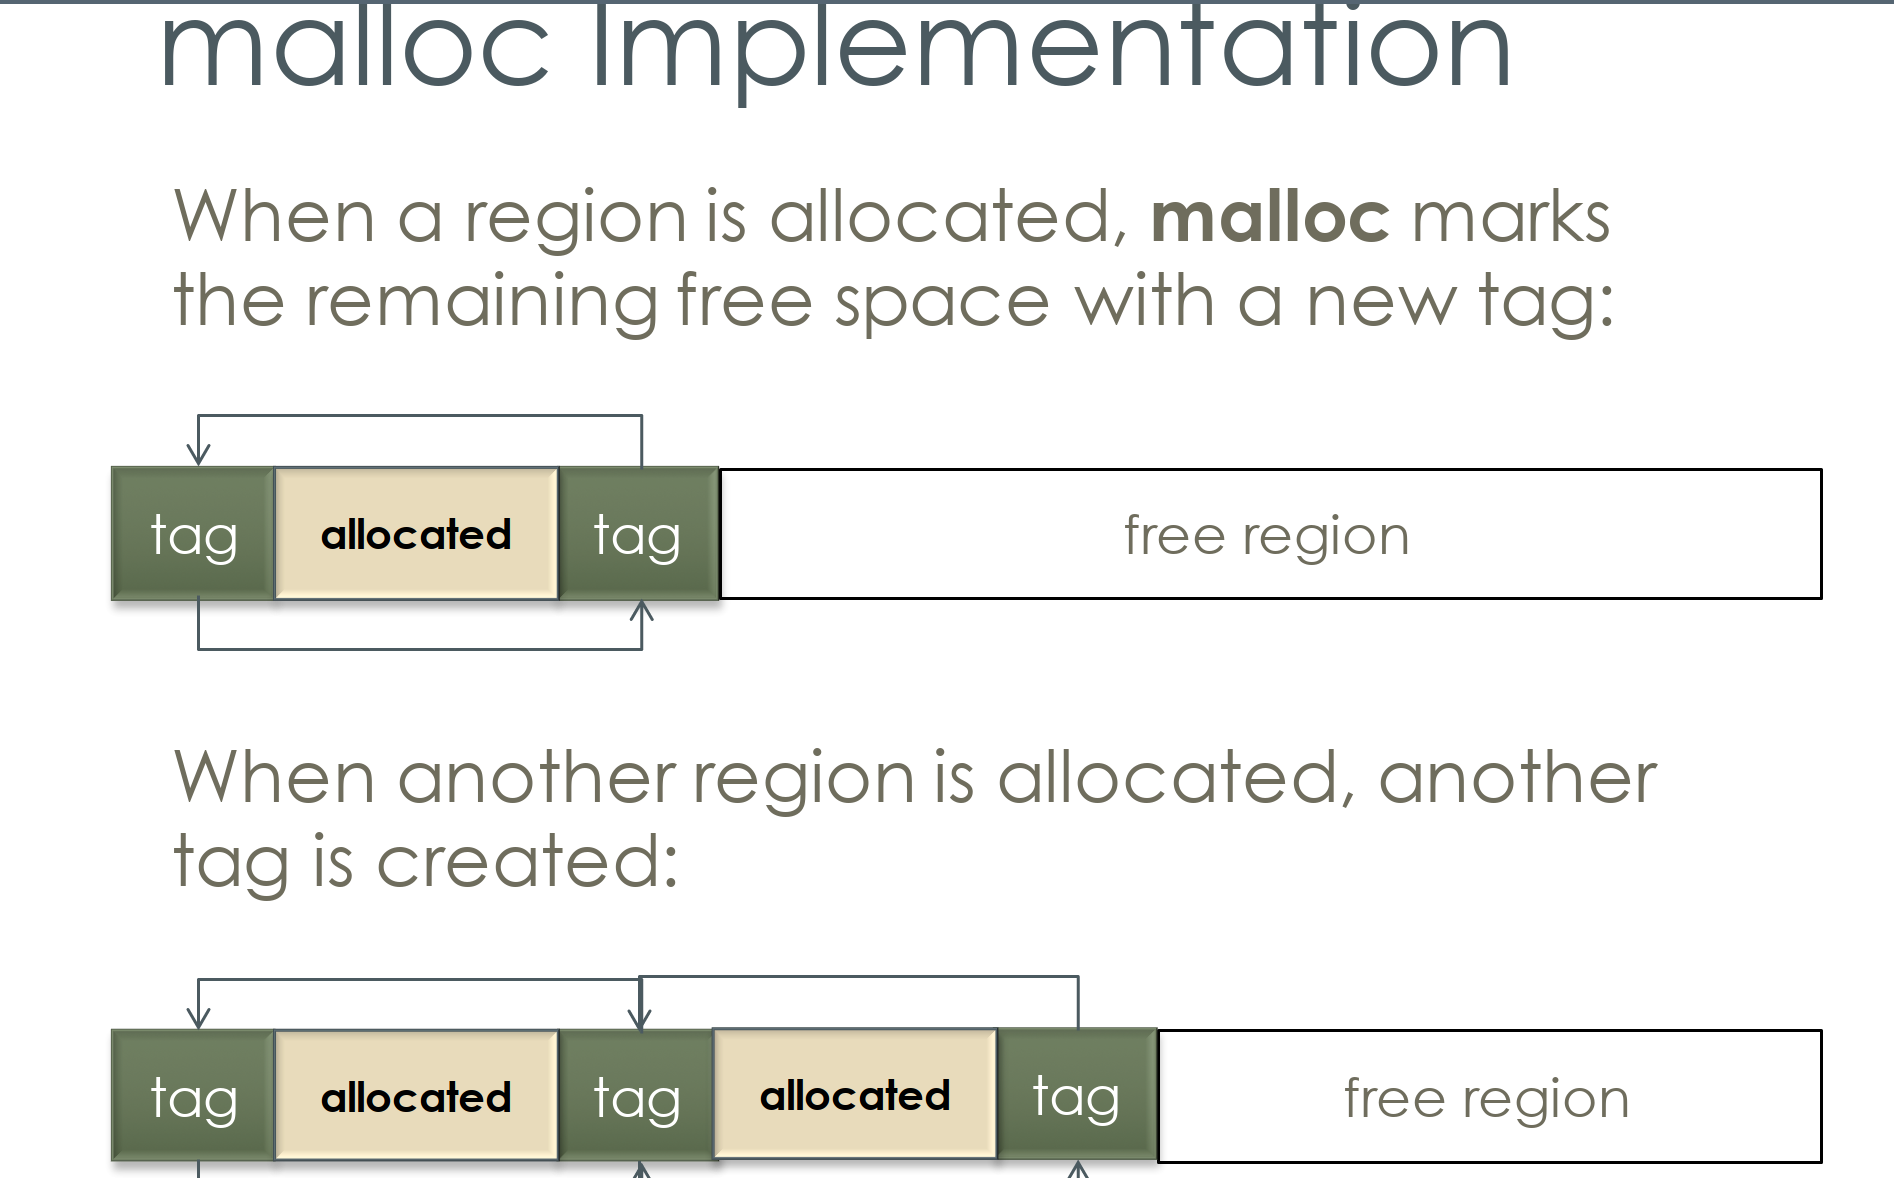
\includegraphics[width=0.8\linewidth]{img/image_2023-01-16-20-09-02.png}
\end{figure}

Malloc places a doubly-linked-list of chunk bits in memory to describe the memory allocated. \texttt{free} sets the free bit, does the various doubly linked list operations (looking at the pointer values of its neighbours in order to remove itself) and also tries to consolidate adjacent free regions.
It assumes that it is passed the beginning of the allocated memory as well as go find the tag associated with the region (which is in a consistent place every time).

The attacker can drop fake tags into memory just ahead of the value we want to overwrite and then we can use the free() call to overwrite memory with the attacker's data.
For example we can create a fake tag node with a prev and next pointer. We make the next pointer be the address of the return address. And then "prev" can contain the address of the start of our shellcode. So freeing on this fake tag will overwrite the return address with the shellcode start.



\begin{blockquote}
    Note that this is not possible with a single free if you are not able to write to negative memory indicies. 
    The part that makes this attack works is that the double free allows the attacker to write a fake tag just before the next tag in a totally valid way. Doing this with a single free would also involve writing to memory that the program doesn't own. (recall: how the memory manager works)
    

\end{blockquote}





\subsection{Other common vulnerabilities}

The attacks we have seen have involved overwriting the return address to point to injecting code. Are there ways to exploit software without injecting code? Yes -- return into \texttt{libc} i.e. use \texttt{libc}'s \texttt{system} library call which looks already like shell code.
This can be accomplished with any of the exploits we have already talked about.

I.e.

\begin{itemize}
    \item Change the return addresses to point to start of the system function
    \item Inject a stack frame on the stack
    \item Before return sp points to $ \&system $
    \item System looks in stack for arguments
    \item System executes the command, i.e maybe a shell
\end{itemize}


\begin{itemize}
    \item Function pointers
    \item Dynamic linking
    \item Integer overflows
    \item Bad bounds checking
\end{itemize}


\subsubsection{Attacks without overwriting the return address}

Finding return addresses is hard. So we can use other methods to inject code into the program.

\begin{itemize}
    \item Function pointers: an adversary can just try to overwrite a function pointer
    \item An area where this is very common is with \textit{dynamic linking}, i.e. functions such as \textit{printf}. 
    \item Typically both the caller of the library function and the function itself are compiled to be position independent
    \item We need to map the position independent function call to the absolute location of the function code in the library
    \item The dynamic linker performs this mapping with the procedure linkage table and the global offset table
        \begin{itemize}
            \item GOT is a table of pointers to functions; contains absolute mem location of each of the dyn-loaded library functions
            \item PLT is a table of code entries: onee per each library function called by program, i.e. sprintf@plt
            \item Similar to a switch statement
            \item Each code entry invoes the function pointer in the GOT
            \item i.e. sprintf@plt may invoke jmp GOT[k] where k is the index of sprintf in the GOT
            \item So if we change the pointers in the offset table we can make the program call our own code, i.e. with objdump.\mn{PLT/GOT always appears at a known location.}

        \end{itemize}
\end{itemize}




\subsubsection{Return-Oriented Programming}
\begin{itemize}
    \item An exploit that uses carefully-selected sequences of existing instructions located at the end of existing functions (gadgets) and then executes functions in an order such that these gadgets compose together to deliver an exploit. 
    \item This can be done faster by seeding the stack with a sequence of return addresses corresponding to the gadgets and in the order we want to run them in.
\end{itemize}


\subsubsection{Deserialization attacks}

\begin{itemize}
    \item Serialization is the process of transforming objects into a format that can be stored or transmitted over a network, i.e. to/from JSON.
    \item The attacker knows that the library has a vulnerability in the deserialization process and they can exploit it by passing carefully created data to it.
\end{itemize}


\subsubsection{Integer overflows}

\begin{itemize}
    \item A server processes packets of variable size
    \item First 2 bytes of the packet store the size of the packet to be processed
    \item Only packets of size 512 should be processed
    \item Problem: what if we end up overflowing the integer with a negative value which would cause memcpy to copy over a lot more memory than intended.
\end{itemize}

\begin{listing}[H]
\begin{minted}{c}
char* processNext(char* strm){
    char buf[512];
    short len = *(short*)strm; // note that by default these are signed
    if (len <= 512) {
        memcpy(buf, strm, len); // note that the 3rd arg of memcpy is an unsigned int
        process(buf);
        return strm + len;
    } else {
        return -1
    }
}
\end{minted}
\end{listing}



\subsubsection{IoT}


\subsection{Case Study: Sudo}

A common program attackers target are programs that regular users can run in order to take on elevated privileges.
In \texttt{unix} systems one such program is \texttt{sudo}, for which vulnerability CVE-2021-3156 was discovered in 2021 after lying in there for over 10 years.


\begin{itemize}
    \item \texttt{sudo} will escape certain characters such as "
    \item Someone introduced debug logic called user\_args and then copies in the contents of \texttt{argv}, while un-escaping meta-characters
    \item Bug: if any command-line arg ends in a single backslash, then the null-terminator gets un-escaped and then \texttt{user\_args} keeps copying out of bounds characters onto the stack
    \item I.e. \texttt{sudoedit -s '\textbackslash' \$(perl -e print "A"x1000\$)}
    \item Attacker controls the size of \texttt{user\_args} buffer they overflow. Can control size and contents of the overflow itself; last command-line argument is followed by the environment variables
    \item  Had many exploit options
        \begin{itemize}
            \item Overwrite next chunk's memory tag (same as use-after-free)
            \item Function pointer overwrite one of sudo's functions
            \item Dynamically-linked library overwrite
            \item Race condition a temp file sudo creates
            \item Overwrite the string "usr/bin/sendmail" with the name of another executable, maybe a shell
        \end{itemize}
\end{itemize}


\subsection{Case Study: Buffer overflow in a Tesla}

\texttt{ConnMann} (Connection Manager) is a lightweight network manager used in many embedded systems, i.e. nest thermostats and Teslas for that manager.



In this particular vulnerability the attacker took advantage of the DNS protocol.
DNS responses include a special encoding for the hostnames which help the receiver parse the response and allocated appropriately sized buffers. For example www.google.com is encoded as 3www6google3com.
This response also often contains a lot of repetitive information, so there is some compression is used in the encoding as well. The one we're interested in here is the compression of names by encoding them as a special "field length" of 192 followed by the offset of the other copy of the name -- which enables repetitions to be encoded as 2 bytes.

CVE-2021-26675 was reported by Tesla in 2021 as a bug in ConnMan which allows an malicious DNS reply to uncompress into a large string that can overflow an internal buffer.
This means that a remote attacker who can control or fake a DNS response could perform a buffer overflow on ConnMan -- which runs with root privileges.

\begin{figure}[H]
    \centering
    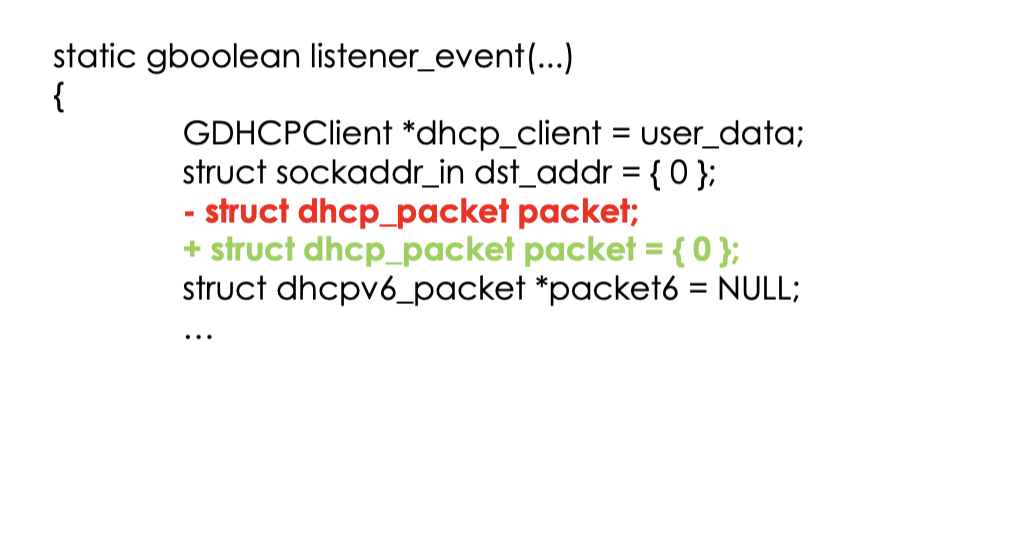
\includegraphics[width=0.8\linewidth]{img/image_2023-01-23-19-05-37.png}
    \caption{ConnMan doesn't initialize the dhcp\_packet struct to 0, which can cause it to leak stack values to a remote attacker (but here they must be on the same subnet as the victim). This vulnerability can be difficult to detect since nobody checks if things are zero in the tests.}
\end{figure}


\begin{blockquote}
    \textbf{So you want to a hack a tesla?}
    \begin{itemize}
        \item Look at the situation; see what kind of protocols being used, etc. Get excited if it uses something old and inane
        \item Look at the data coming in and our, especially if there's any extra going in or out
        \item Use fuzzing tools
        \item Get a sense of what they are expecting us to do as well as what are ways that we can break that example. For example is the only verification just some client-side JavaScript?
        \item Break stuff
    \end{itemize}
\end{blockquote}





\subsection{Fault Injection Attacks}

We make a lot of assumptions about how the underlying systems work. For example proper CPU operation.
Fault injection attacks take advantage of these assumptions by injecting faults into the system, often at the hardware level.

For example: proper pipelined CPU operation depends on stable power and clock inputs.
If the glitch duration is longer than the time it takes to increment the PC and shorter than the instruction fetch time, then we can start to see a special case: instruction skipping or instruction corruption.p


\begin{figure}[H]
    \centering
    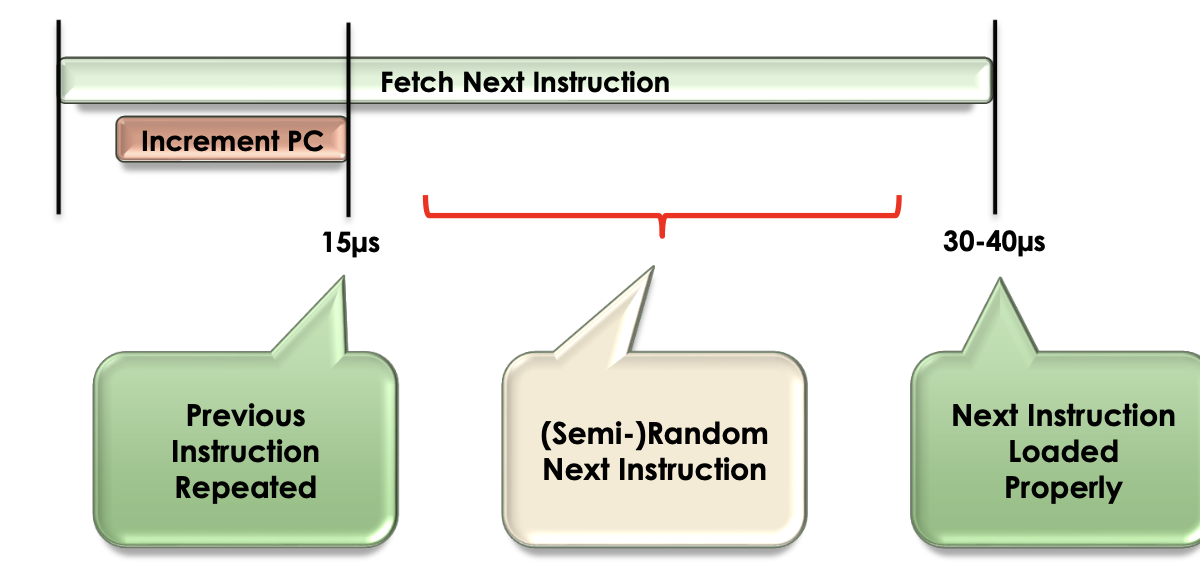
\includegraphics[width=0.8\linewidth]{img/image_2023-01-23-19-40-51.png}
    \caption{With some careful timing we can cause the CPU to skip or repeat an instruction.}
\end{figure}

\begin{figure}[H]
    \centering
    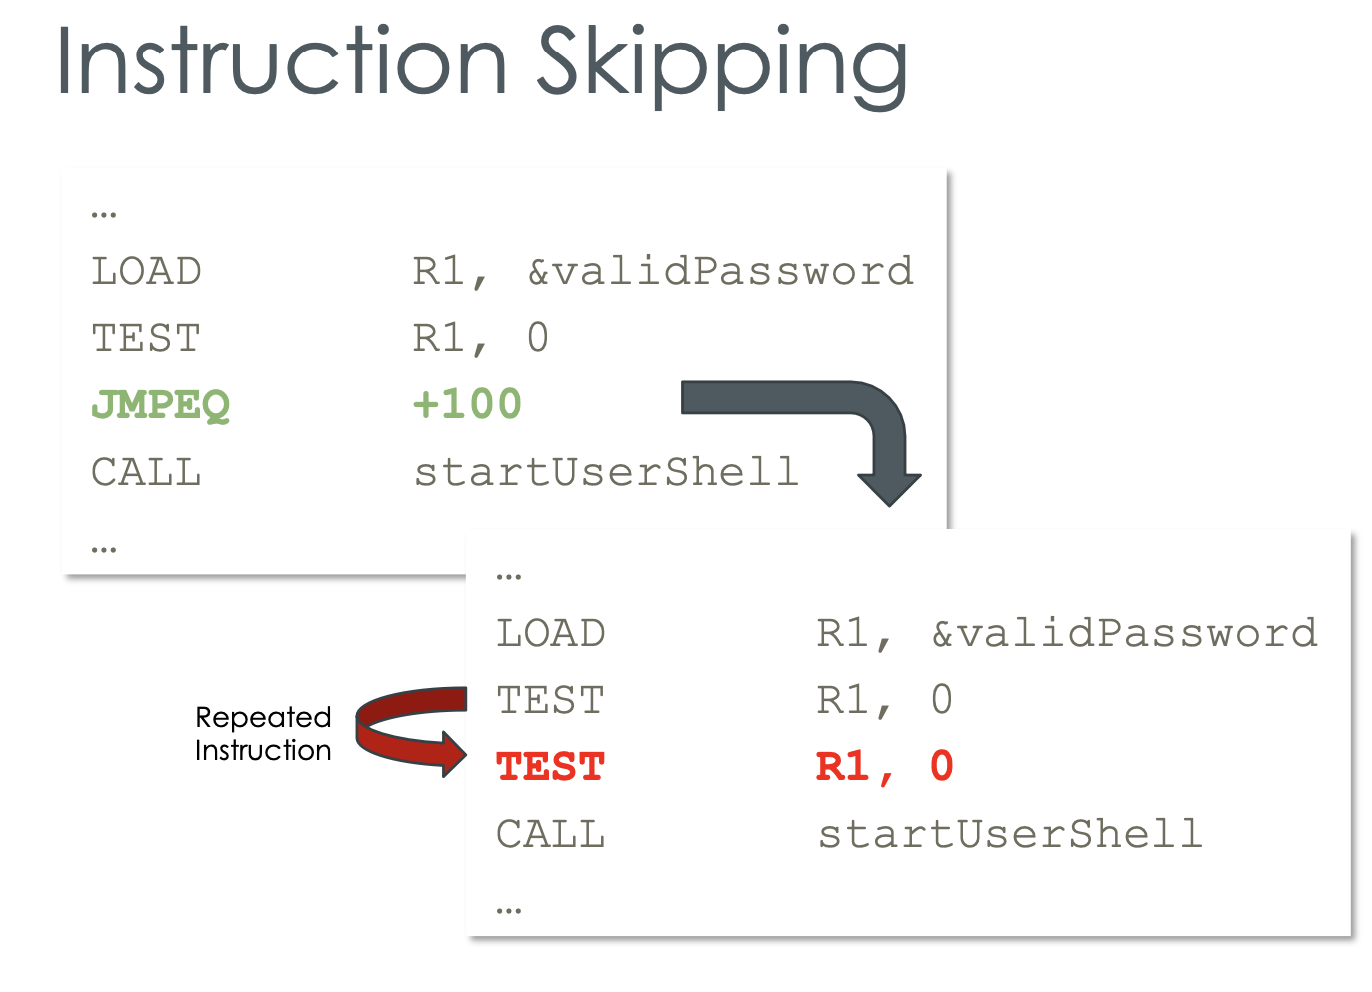
\includegraphics[width=0.8\linewidth]{img/image_2023-01-23-19-41-31.png}
    \caption{An example of where this can be useful: skipping the JMP instruction of an IF statement}
\end{figure}


\subsubsection{Hardware Demo}


Consider this simple program that checks a text buffer for a password and then logs you in if it's correct

\begin{figure}[H]
    \centering
    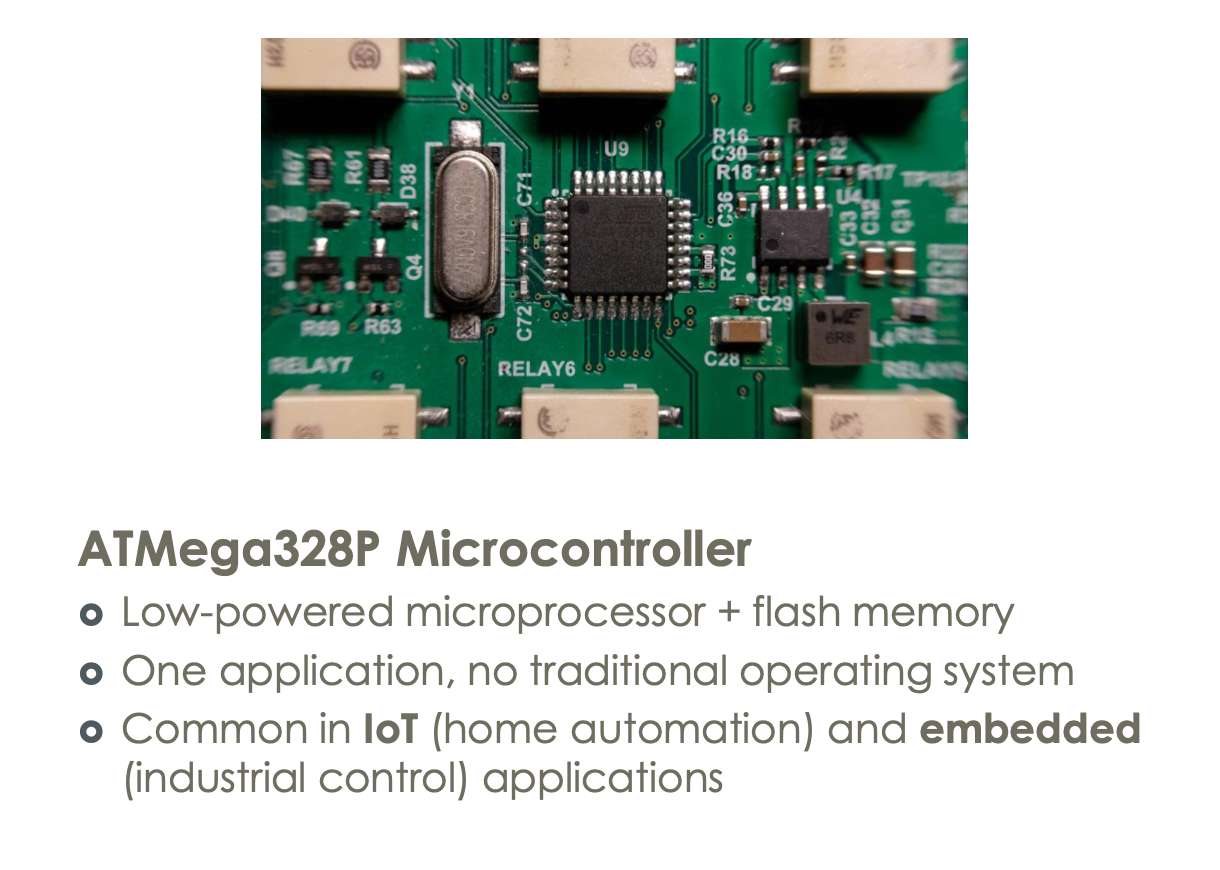
\includegraphics[width=0.8\linewidth]{img/image_2023-01-23-19-44-00.png}
\end{figure}

\begin{figure}[H]
    \centering
    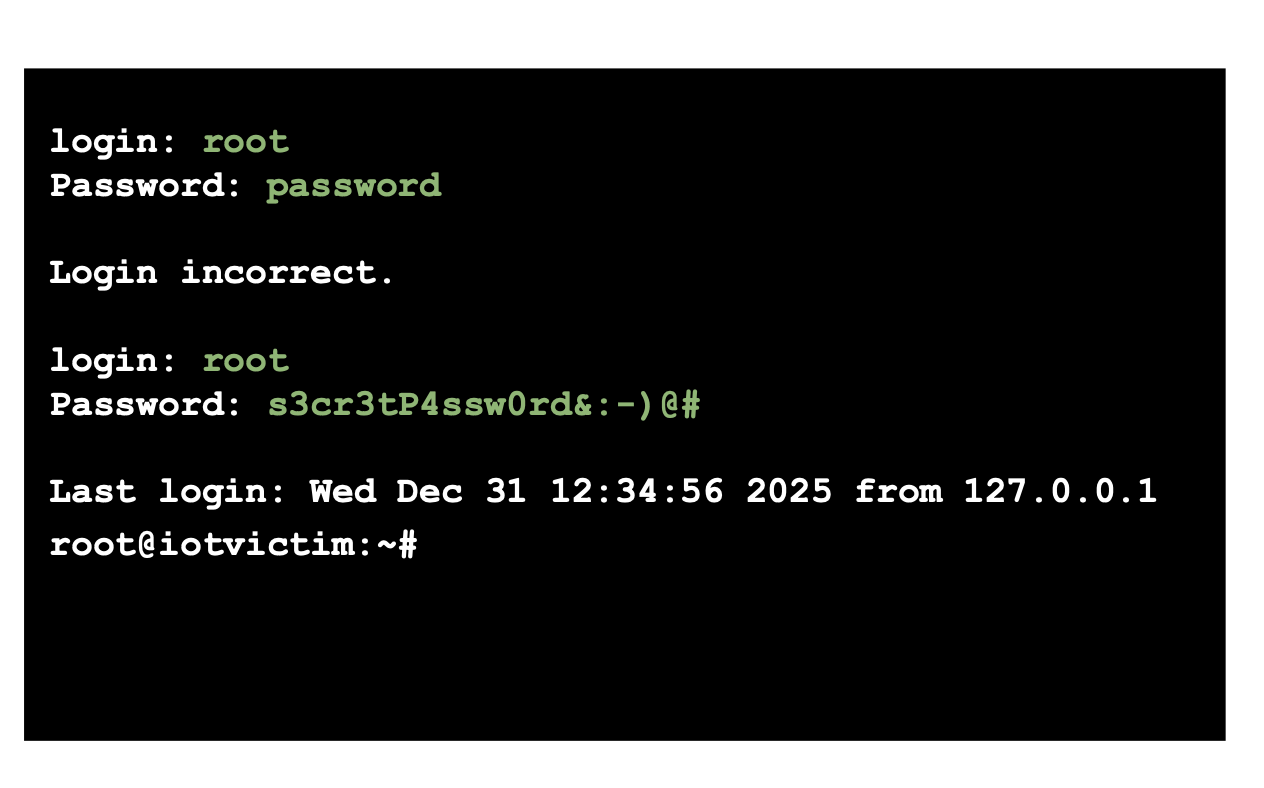
\includegraphics[width=0.8\linewidth]{img/image_2023-01-23-19-44-33.png}
\end{figure}
\begin{figure}[H]
    \centering
    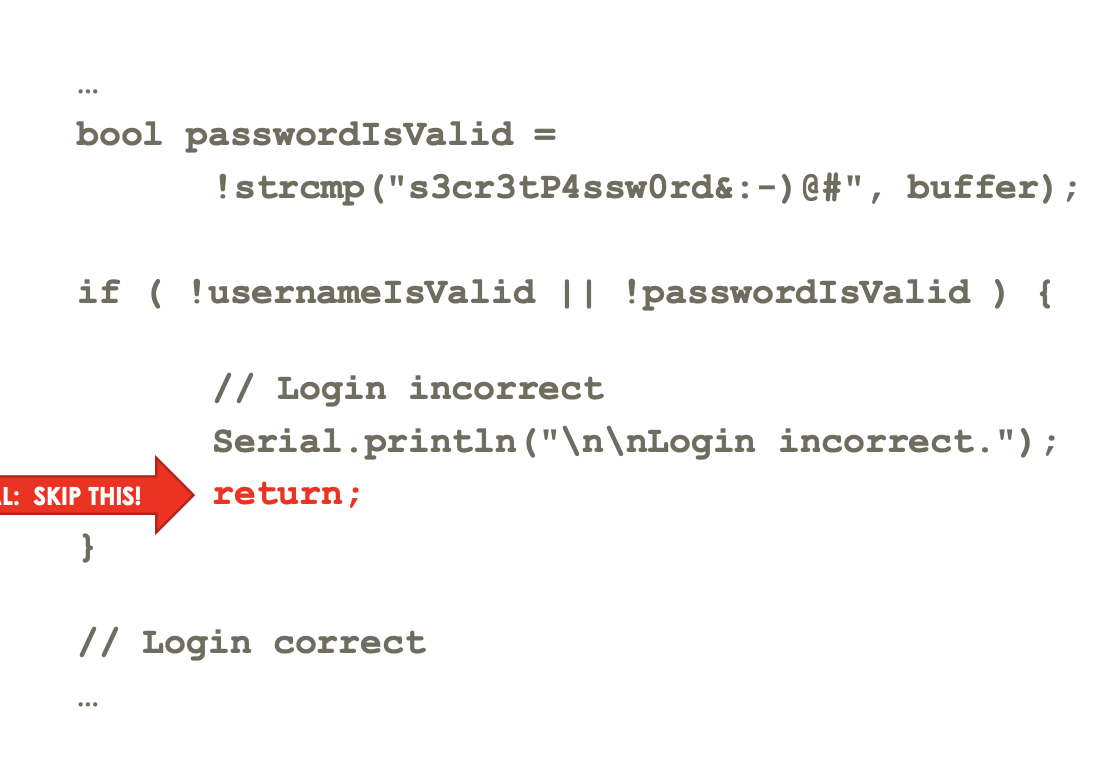
\includegraphics[width=0.8\linewidth]{img/image_2023-01-23-19-44-46.png}
\end{figure}

\begin{figure}[H]
    \centering
    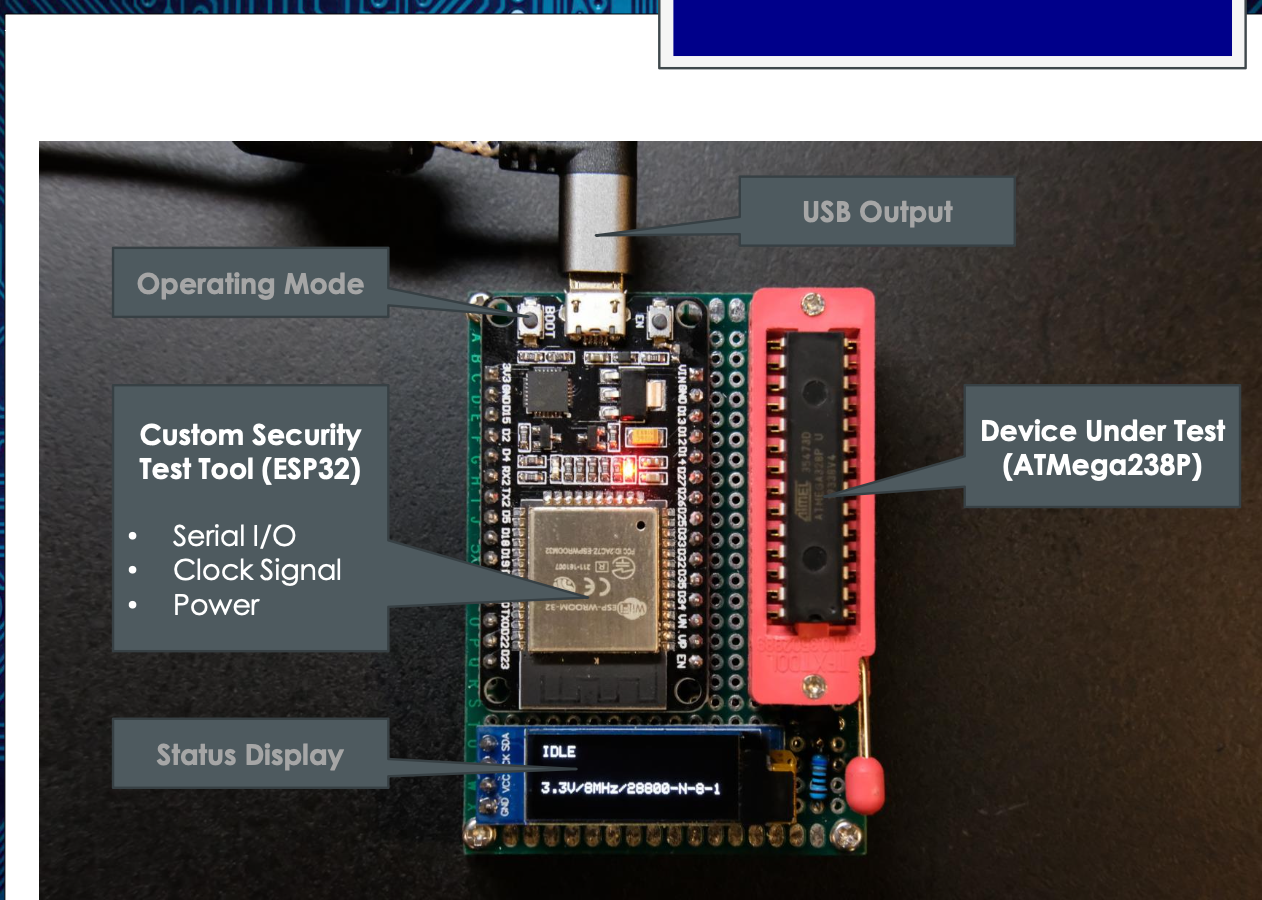
\includegraphics[width=0.8\linewidth]{img/image_2023-01-23-19-45-52.png}
    \caption{The ATMega238P hooked up to a custom security test tool built on top of a ESP32}
\end{figure}


Our attack is to use a \textbf{clock glitch}\mn{A series of very brief and rapid clock pulses} at the time of the return instruction.
Finding the time of the return instruction is a bit tricky but we can just sweep across a range of times.



\begin{figure}[H]
    \centering
    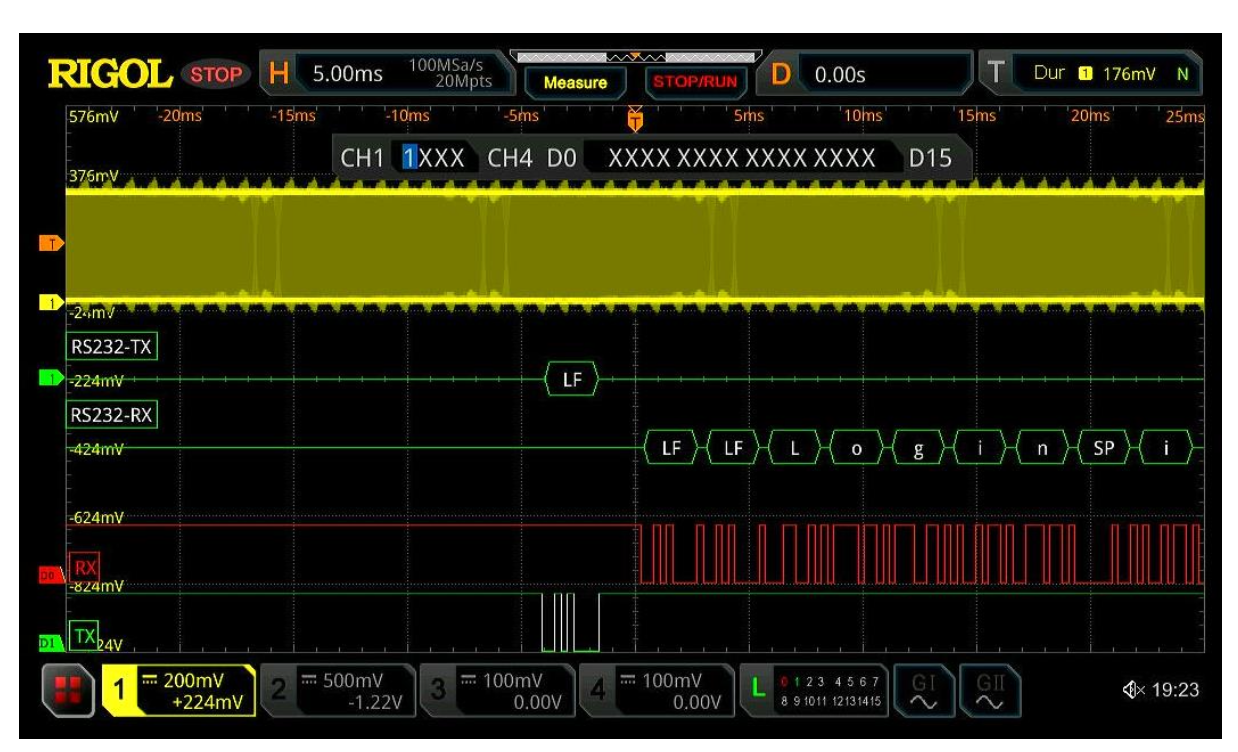
\includegraphics[width=0.8\linewidth]{img/image_2023-01-23-19-52-22.png}
    \caption{Looking at the oscilloscope to show the sweeped input}
\end{figure}


\begin{figure}[H]
    \centering
    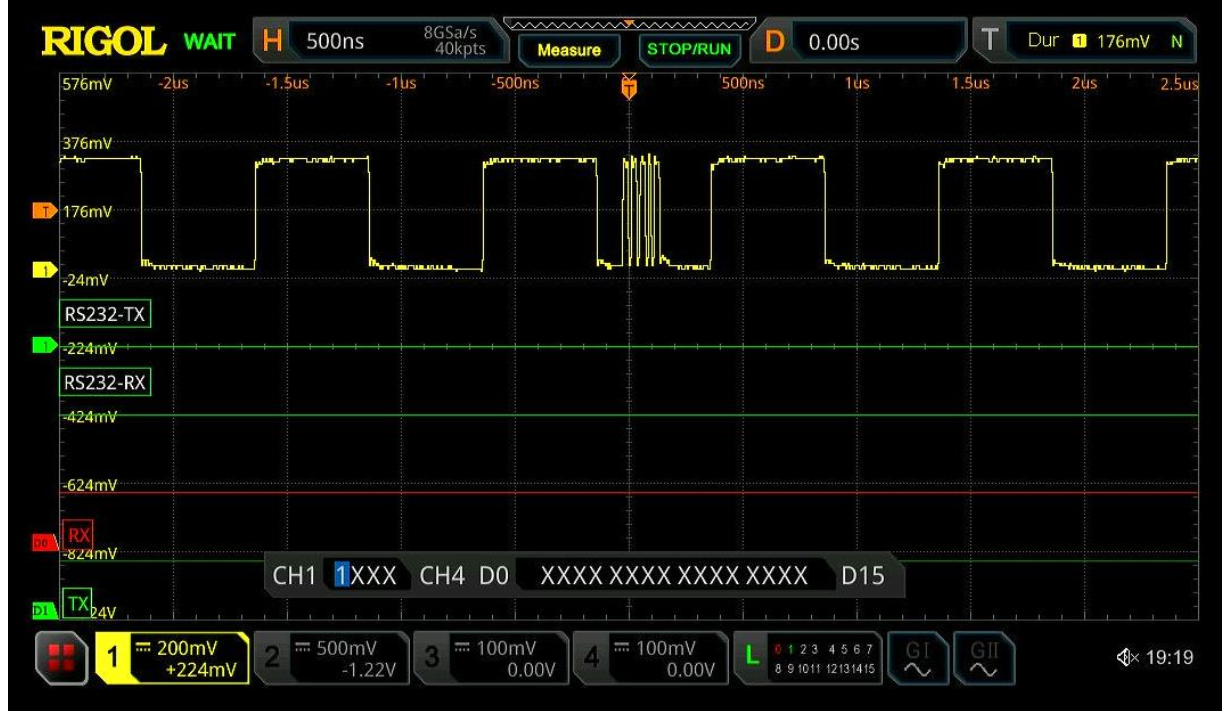
\includegraphics[width=0.8\linewidth]{img/image_2023-01-23-19-53-10.png}
    \caption{Note crazy clock pulses which we try to line up with the return instruction. If we have a really good chip we can try it with only 1 pulse, but here we use 5 pulses because we're on a cheaper chip. We also don't happen to care too much about whether or not if we disrupt too many of the other instructions.}
\end{figure}



Another attach that is a bit easier to use is the \textbf{power glitch}: instead of not giving it enough time for the fetch to happen we take away the nice voltage going to the chip right at the instruction execution time. 

\begin{figure}[H]
    \centering
    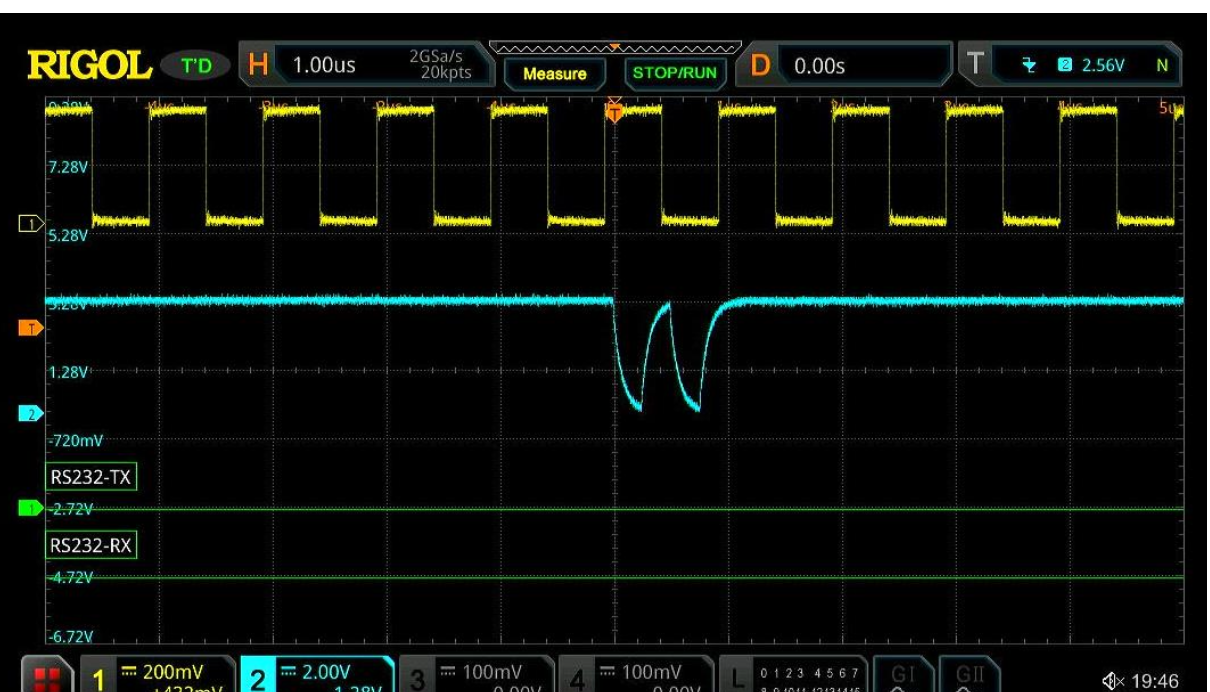
\includegraphics[width=0.8\linewidth]{img/image_2023-01-23-19-59-04.png}
    \caption{A power glitch attack disrupts the fetch instruction or the decode}
\end{figure}

Defense for these attacks is to disallow physical access to the chip. For the power one it can be as simple as adding a little capacitor to the power supply to smooth it out.
Likewise, there are many ways to cause controlled circuit malfunctions: lasers, strobes, EM pulses, etc.


\subsection{Reverse Engineering}

Reverse Engineering, or the act of analyzing a product in order to learn something about its design which its creator wanted to keep secret.
It is a legally complicated, but generally it's ok for the purposes of achieving interoperability (but not for circumventing DRMs).


\begin{listing}[H]
\begin{minted}{c}
unsigned int printhelloworld() {
    printf("Hello World!");
    return 5;
}
int main (int argc, char *argv[]) {
    unsigned int result = 0;
    result = printhelloworld();
    if (result == 4) {
        printf("super secrete string\n");
    }
    return 0;
}
\end{minted}
\end{listing}


\begin{figure}[H]
    \centering
    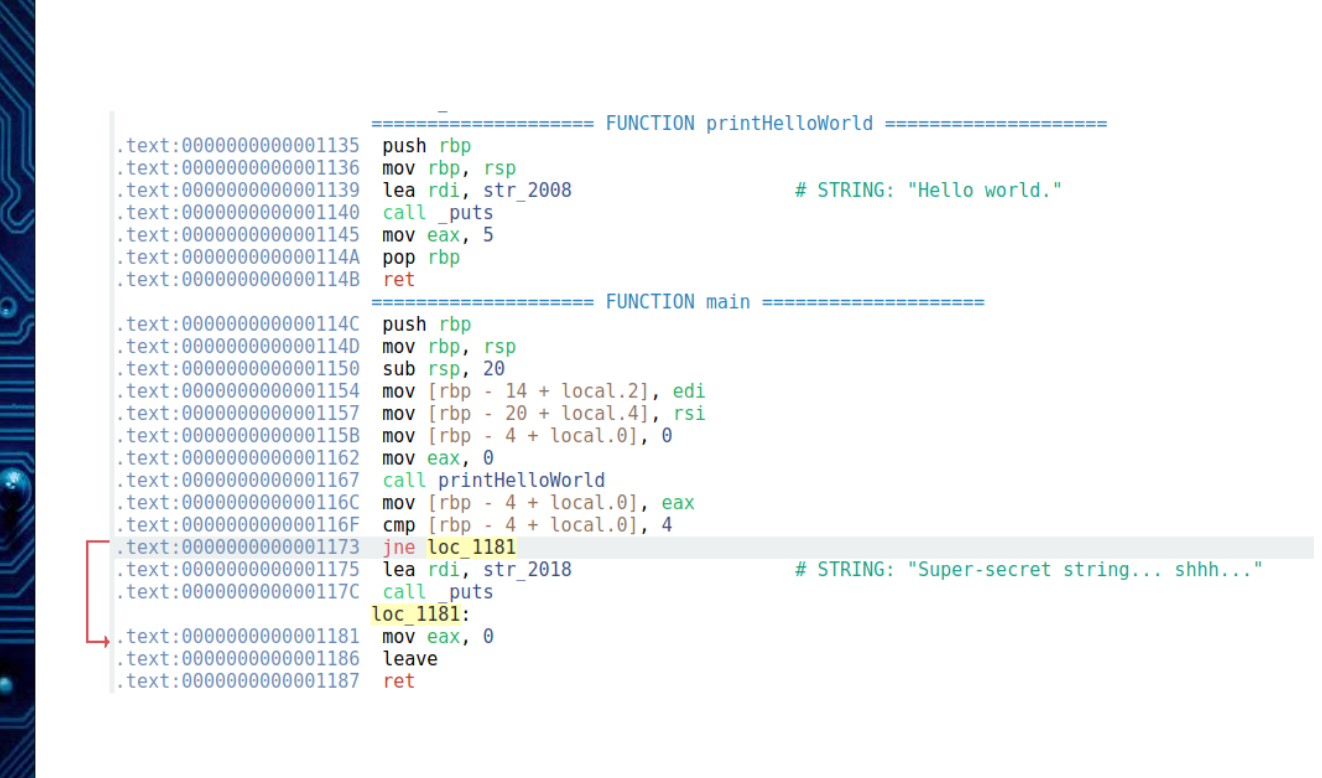
\includegraphics[width=0.8\linewidth]{img/image_2023-01-23-20-35-06.png}
    \caption{Passing the binary compiled from the above code to a disassembler}
\end{figure}

With the disassembled binary we know where the instruction for the if statement we were curious about lives, so we can then just use hexedit to change the bits at that JMP to a NOP to print out the super secret string.


\subsection{Buffer Overflow Defenses}

\begin{itemize}
    \item Audit code rigorously
    \item Use a type-safe language with bounds checking (Java, C\#, rust)
    \item However, this is not always possible due to legacy code, performance, etc.
    \item Defending against stack smashing
        \begin{itemize}
            \item Stackshield: put return addresses on a seperate stack with no other data buffers there
            \item Stackguard: a random canary value is placed just before the RA on a function call. If the canary value changes, the program is halted. This can be enabled via a flag on most modern compilers.
        \end{itemize}
    \item Third-party libc i.e. libsfae which doesn't allow for '\%n` in format strings
    \item Address space layout randomization: maps the stack of each process at a randomly selected location with each invocation, so that an attacker will not be able to easily guess the target address. GCC does do this by default.

\end{itemize}

If we really sit down and think about it, it's basically impossible to defend against all attacks. 
It's easy to make a mistake and end up with a vulnerability. Certain vulnerabilities can be avoided by using safer languages, but the only real defense is to be aware and careful.
One approach is what the aerospace industry does, i.e. the swiss cheese model \mn{if we stack a lot of hole-y cheese on top of each other it will be opaque}


\subsection{Cryptography}



\begin{blockquote}
    \textbf{Case Study: Espressif ESP32} 

    \begin{figure}[H]
        \centering
        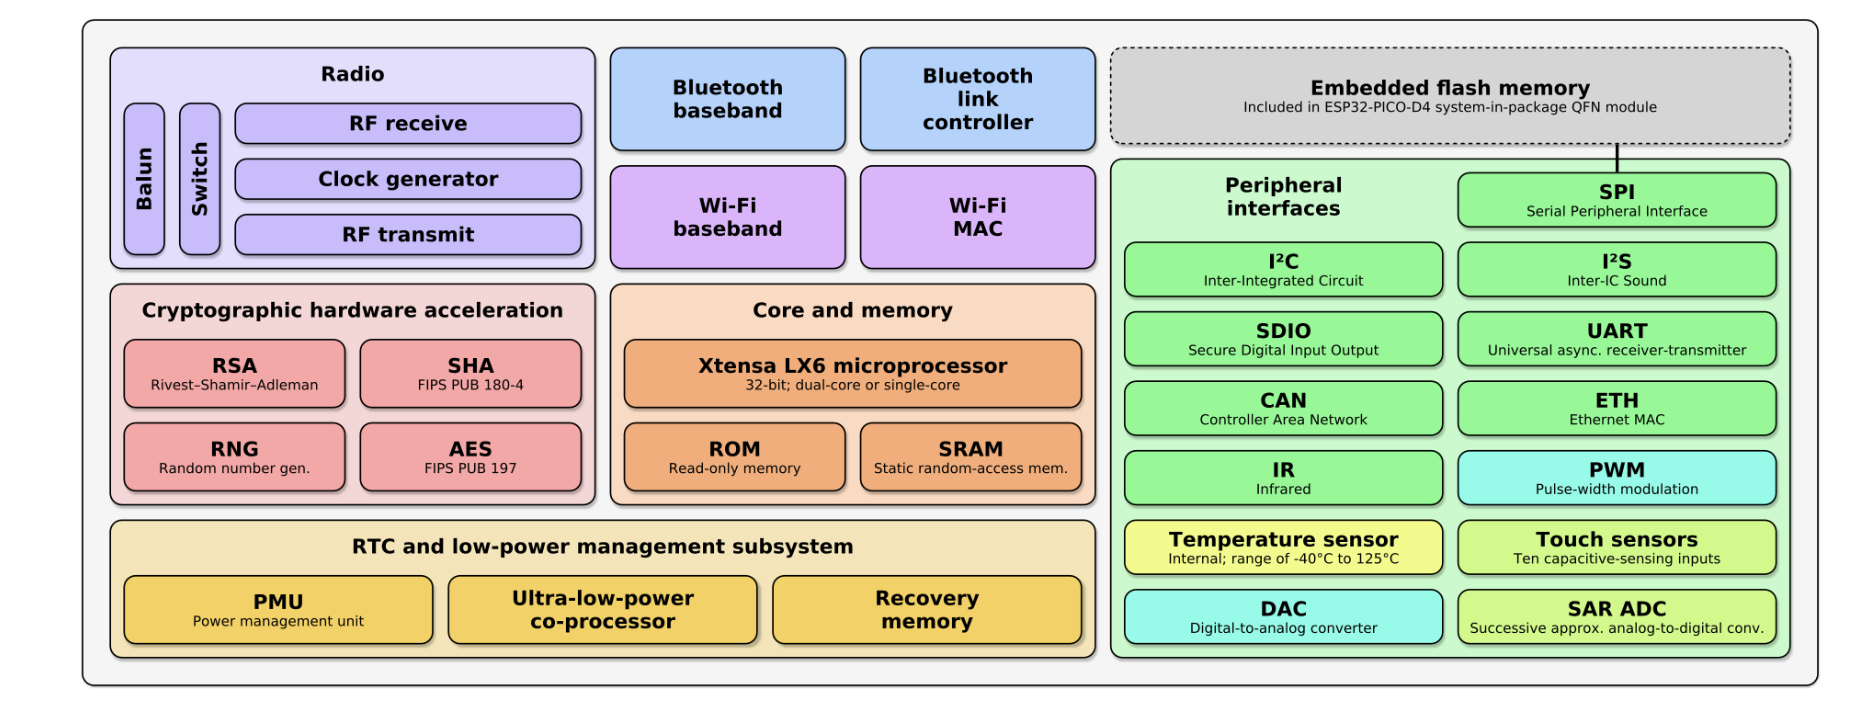
\includegraphics[width=0.8\linewidth]{img/image_2023-01-30-18-19-48.png}
    \end{figure}

    \begin{itemize}
        \item Microcontroller that the prof used for the demo last class
        \item Programming the microcontroller usually happens during the manufacturing phase
        \item Flash memory is usually partitioned into the bootloader, data, and application
        \item In the factory the ESP32 will generate a random number (on first boot) in order which will be used to encrypt and hash the bootloader and the data on the board. Then it starts the applications.
        \item On subsequent boots the device will make recalculate the hash to make sure that the bootloader has not been tampered with.
        \item More information about using PGP encryption for the data partition, etc. Not too important.
        \item TLDR: lots of encryption and security features built into the chip
    \end{itemize}
\end{blockquote}

\begin{blockquote}
    \textbf{Case Study: Door Alarm} 
    \begin{figure}[H]
        \centering
        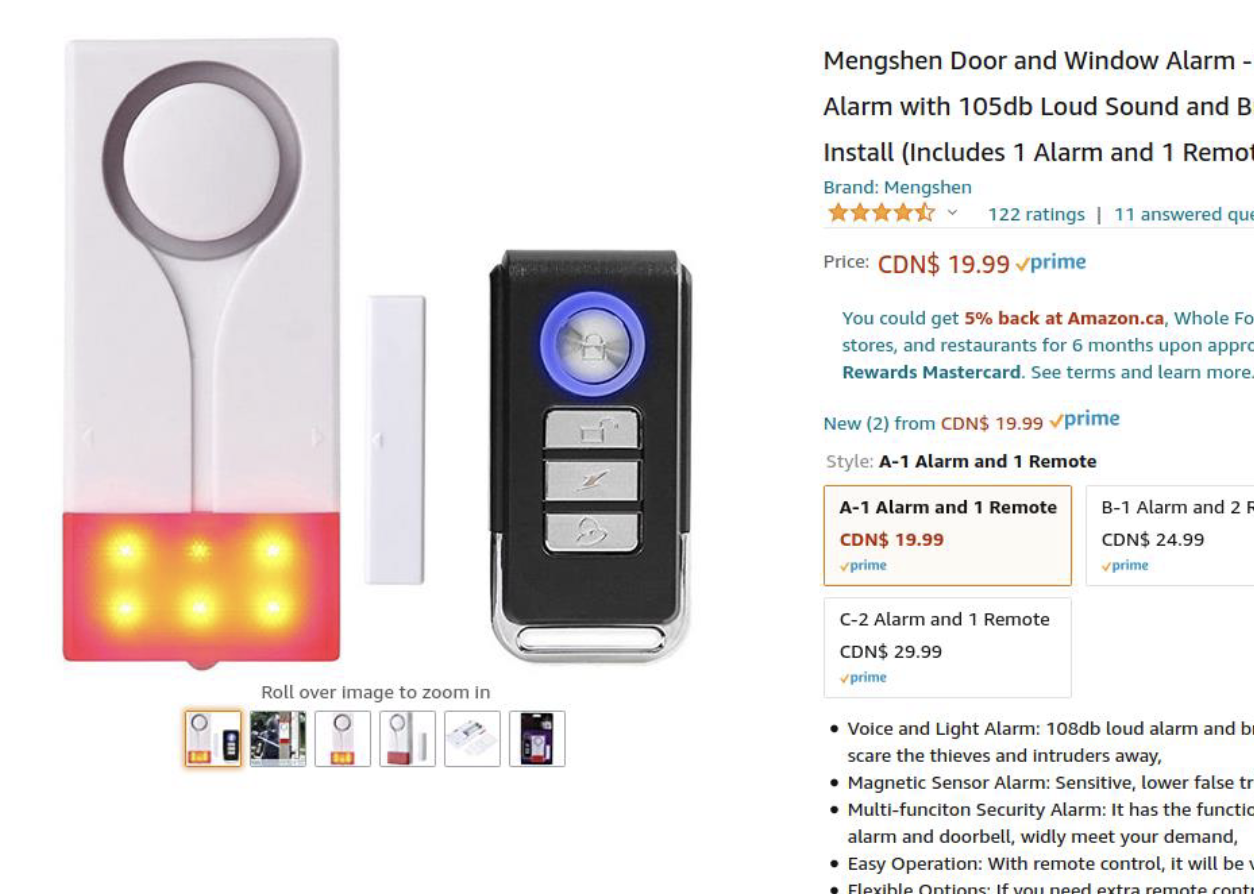
\includegraphics[width=0.8\linewidth]{img/image_2023-01-30-18-43-35.png}
    \end{figure}

    What would a small-scale communication-channel pentest look like for this?


    1. Look at FCC report

    \begin{figure}[H]
        \centering
        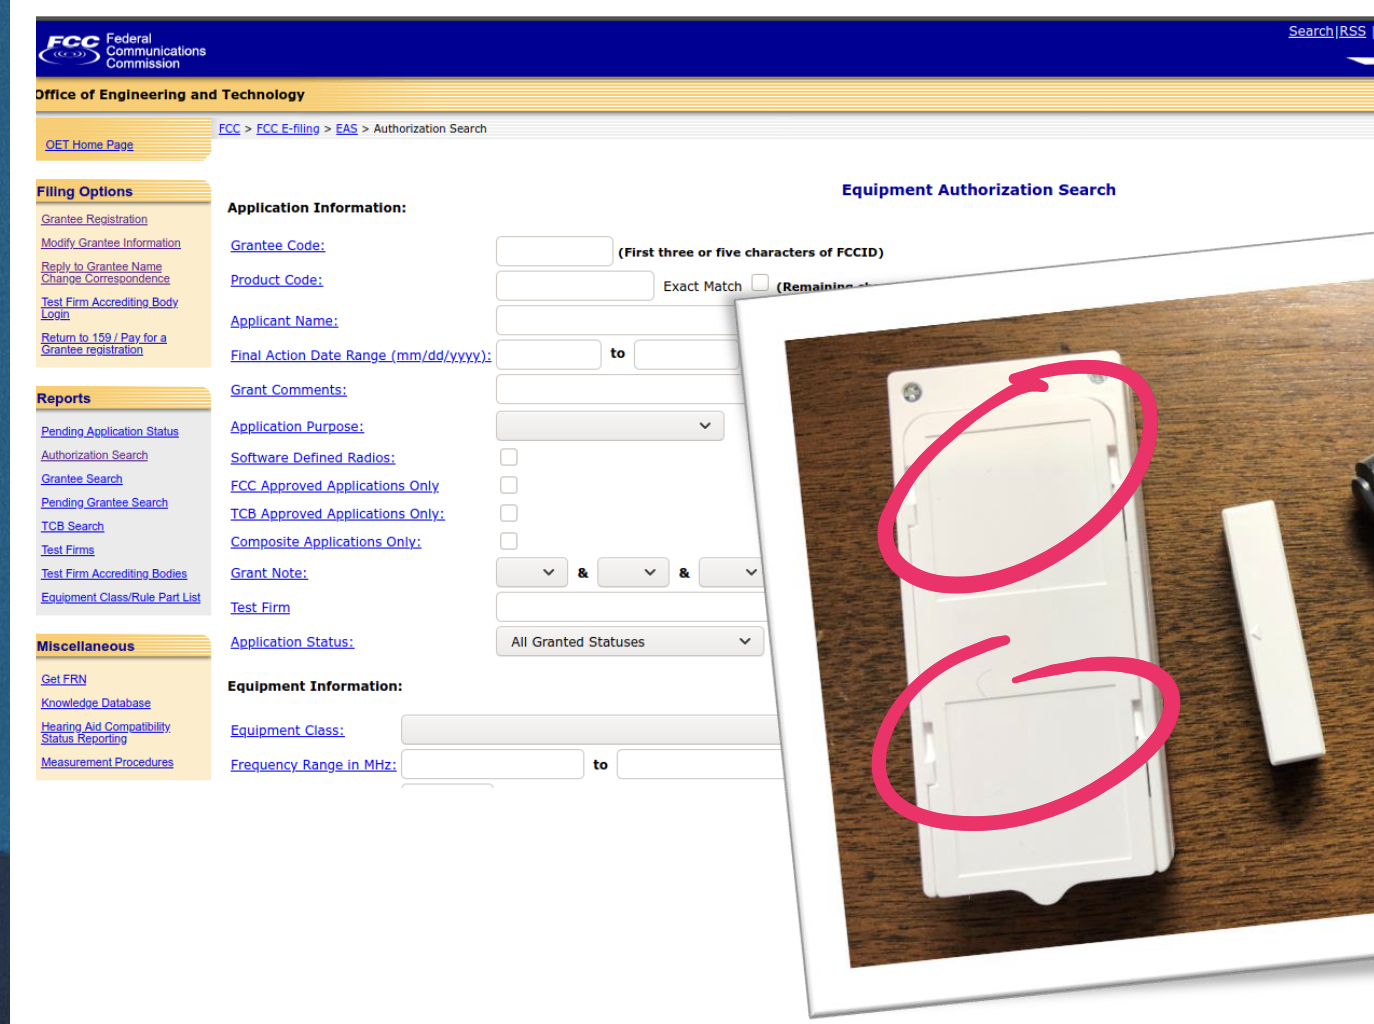
\includegraphics[width=0.8\linewidth]{img/image_2023-01-30-18-45-35.png}
        \caption{In this case this was barely done so it wasn't very useful}
    \end{figure}

    2. Make reasonable guesses

    \begin{figure}[H]
        \centering
        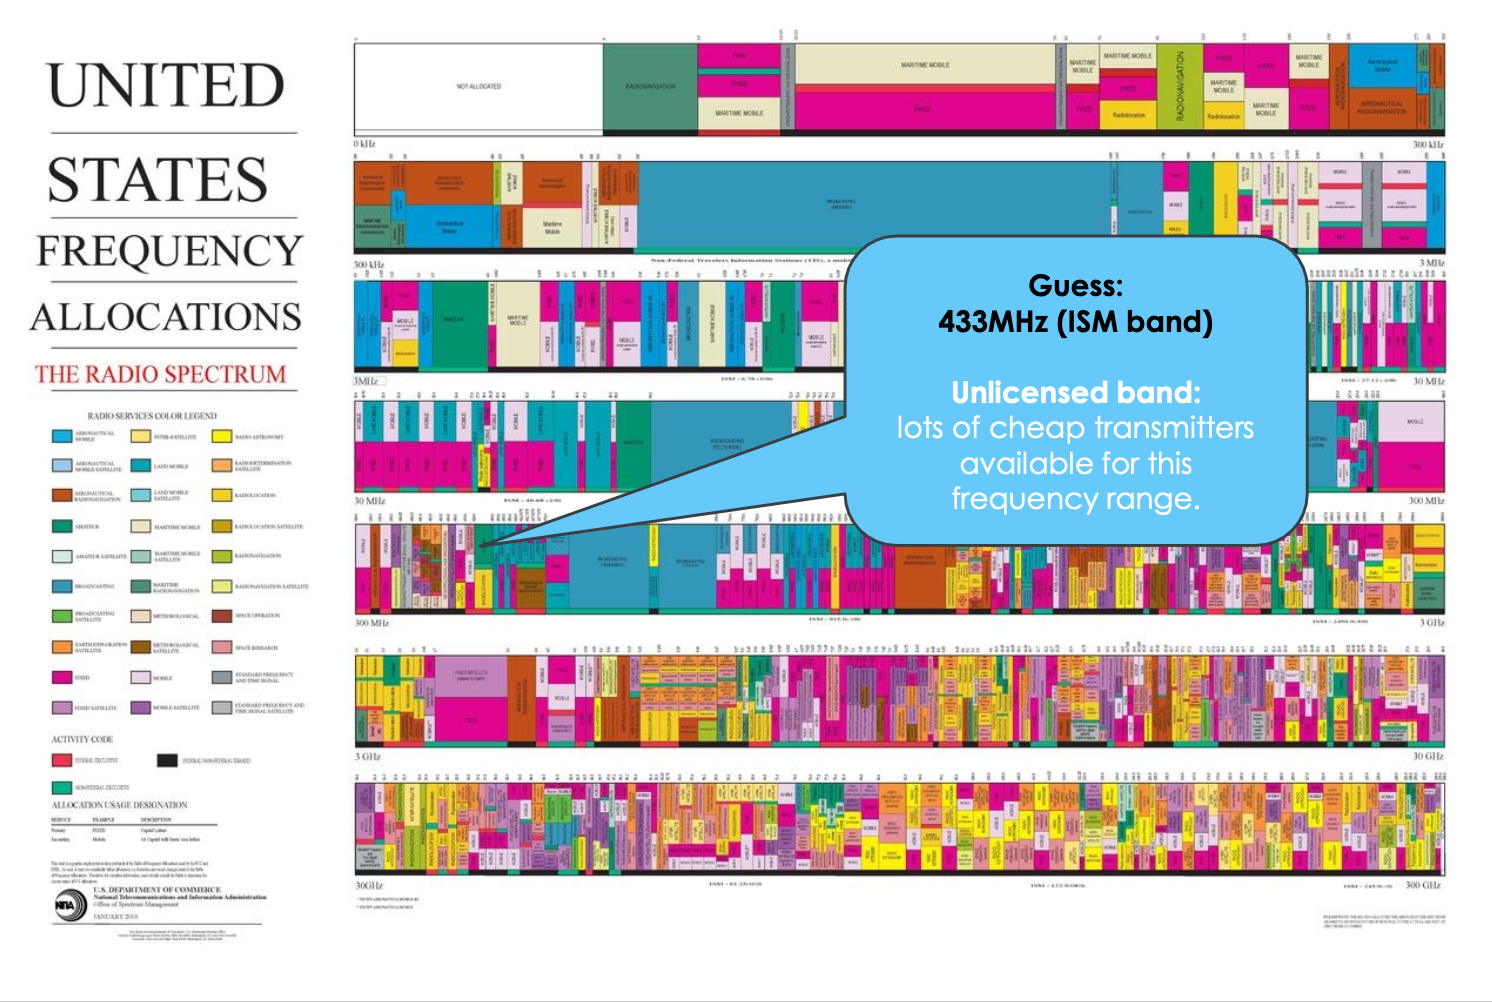
\includegraphics[width=0.8\linewidth]{img/image_2023-01-30-18-46-55.png}
        \caption{Guess that this cheap device is on unlicensed 433 MHz band}
    \end{figure}

    3. Listen into the signal

    \begin{figure}[H]
        \centering
        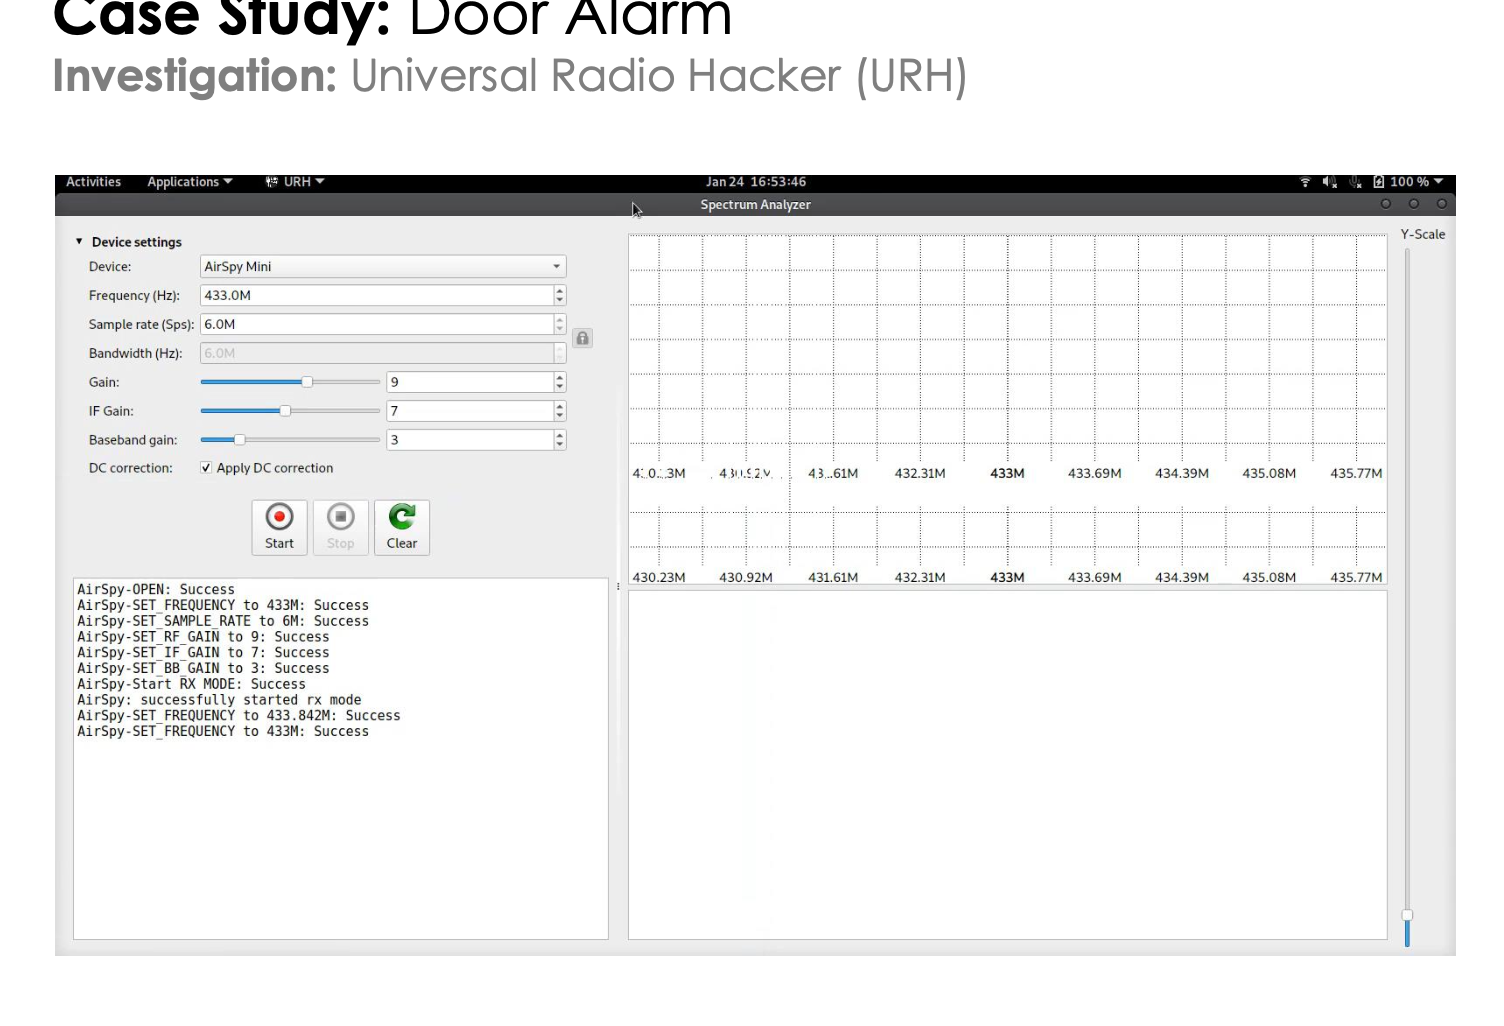
\includegraphics[width=0.8\linewidth]{img/image_2023-01-30-18-47-45.png}
        \caption{Use a software-defined radio to inspect the signal}
    \end{figure}

    \begin{figure}[H]
        \centering
        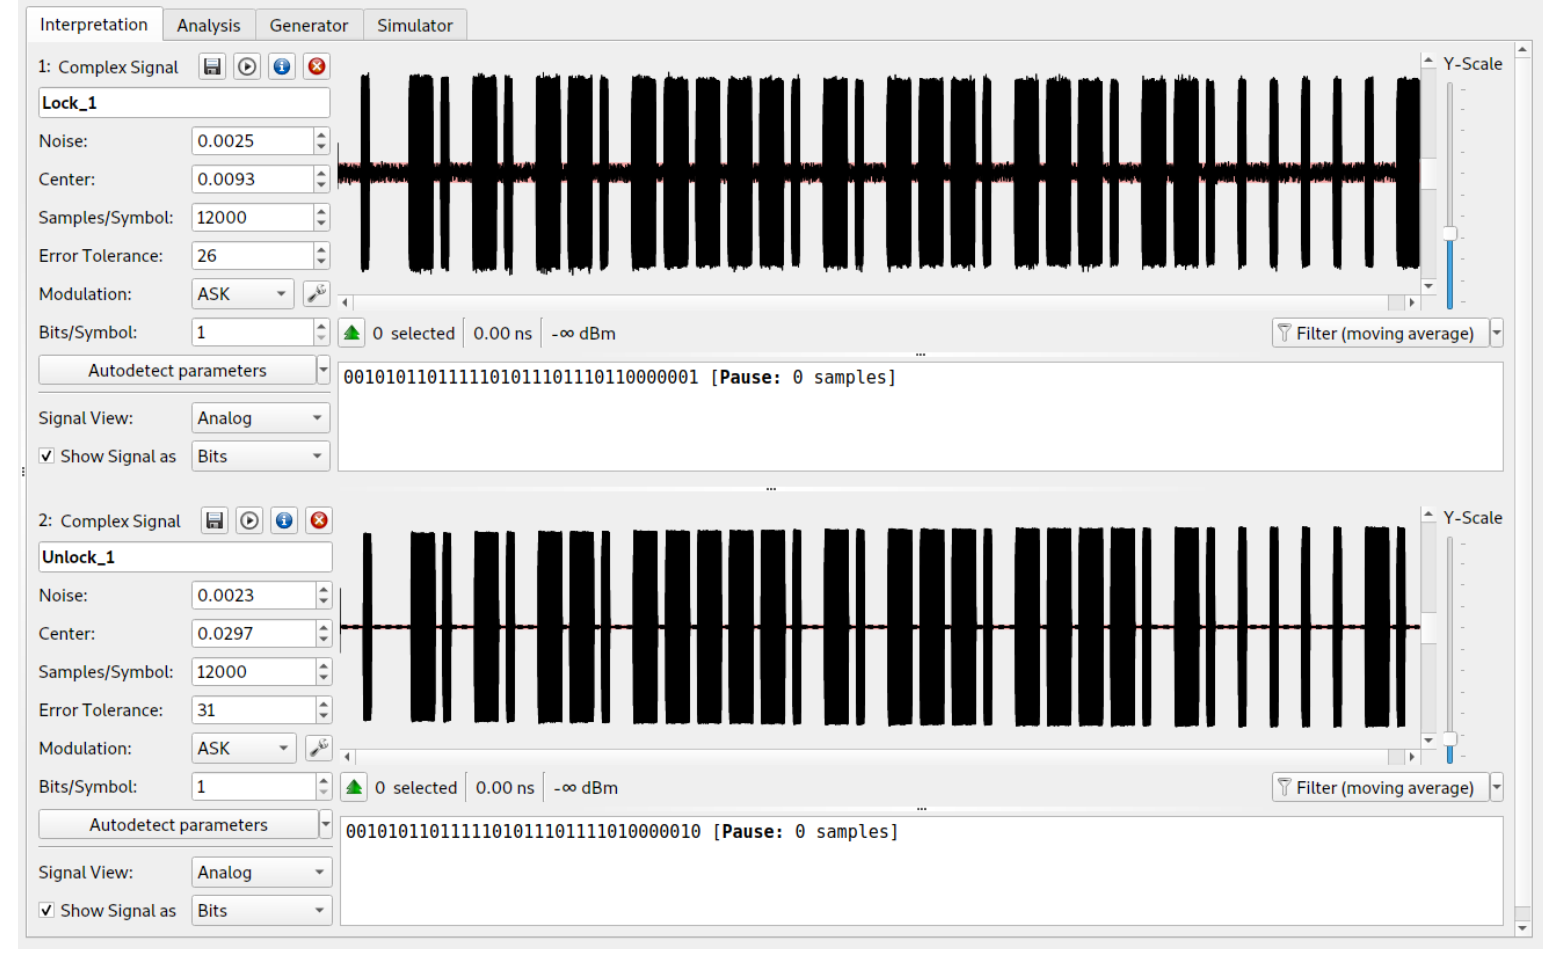
\includegraphics[width=0.8\linewidth]{img/image_2023-01-30-18-48-22.png}
        \caption{Top signal is lock, bottom signal is unlock. Here we don't know what they are yet but there \textit{is} some sort of unique binary pattern being produced on the button clicks.}
    \end{figure}

    4. Replay?

    \begin{figure}[H]
        \centering
        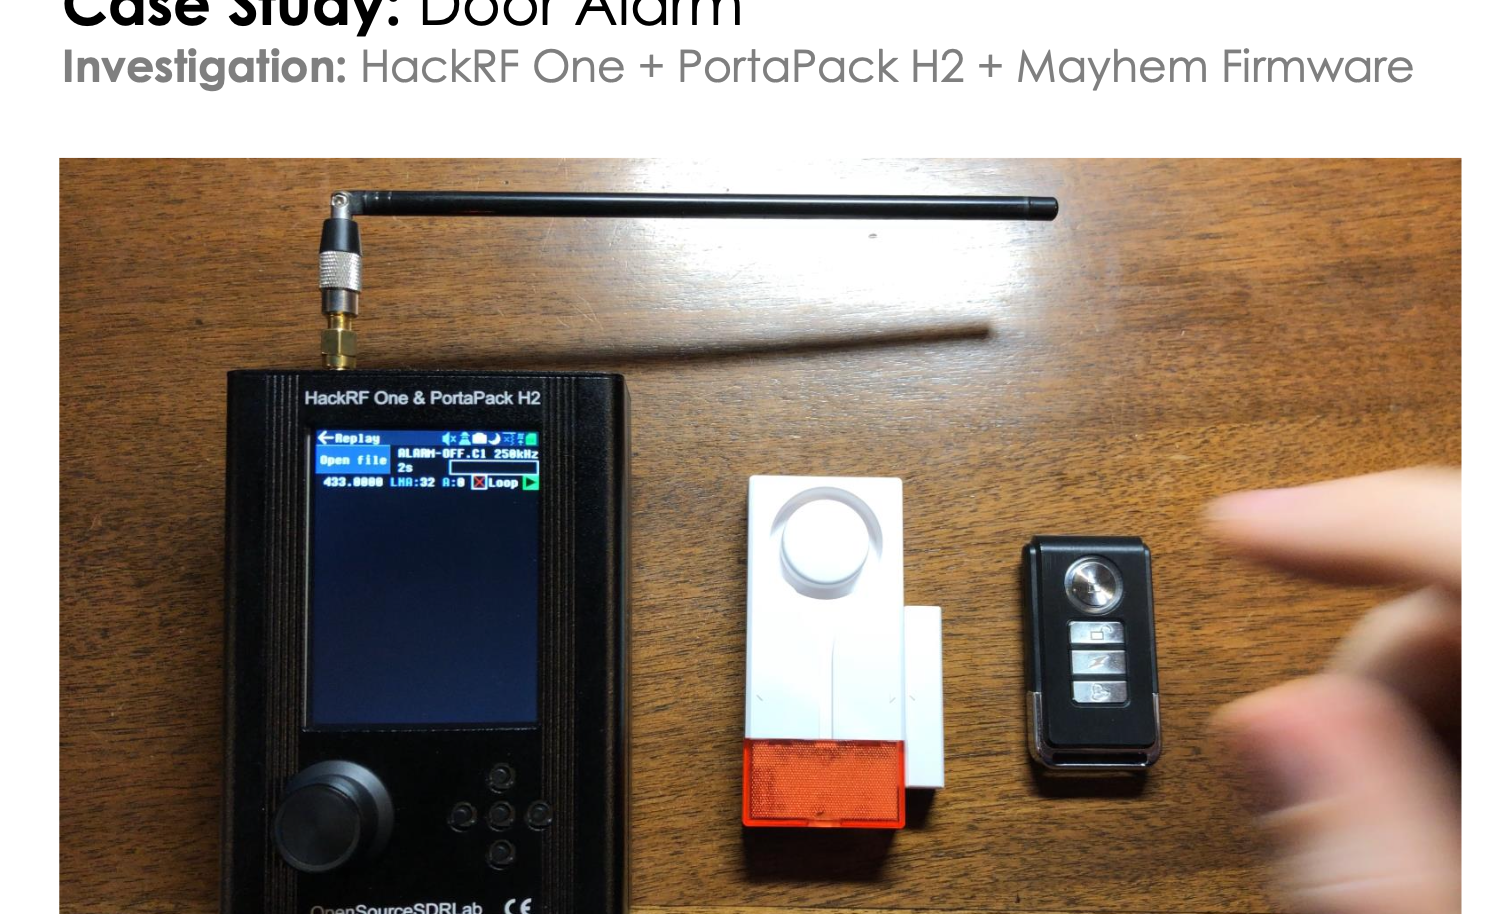
\includegraphics[width=0.8\linewidth]{img/image_2023-01-30-18-50-56.png}
        \caption{Can just use a radio recorder/playback device to record the signal and play it back in order to unlock the doorlock}
    \end{figure}

\end{blockquote}

As it turns out industrial systems tend not be be any more secure


\subsubsection{Ciphers}

Cryptography is used to establish the confidentiality, integrity, authenticity, and non-repudiation\mn{Prevents a principal from denying they have performed an action} of data.

\begin{itemize}
    \item Ciphers an algorithm that obfuscates data so that it seems random to anyone hwo does not possess special information called a key.
    \item Based on a class of functions called trapdoor one-way functions, i.e. easy to compute but inverse is difficult to compute. Trapdoor means that given the key the inverse becomes easy to compute\mn{Note that never been proven/disproven that one-way functions exist. Plus if it's been proved it would show $ P \neq  NP $}
    \item Function itself should not be the critical secret (Kerckhoff's principle)
\end{itemize}

Two common one-way functions used are factoring ($ z=(x*y)$ find x,y) and discrete log ($z= x^y \% m $ -- given z, x, m, find $ y = \log_x z \% m $)

\begin{definition}
    \textbf{Caesar (Shift) Cipher} 

    \begin{figure}[H]
        \centering
        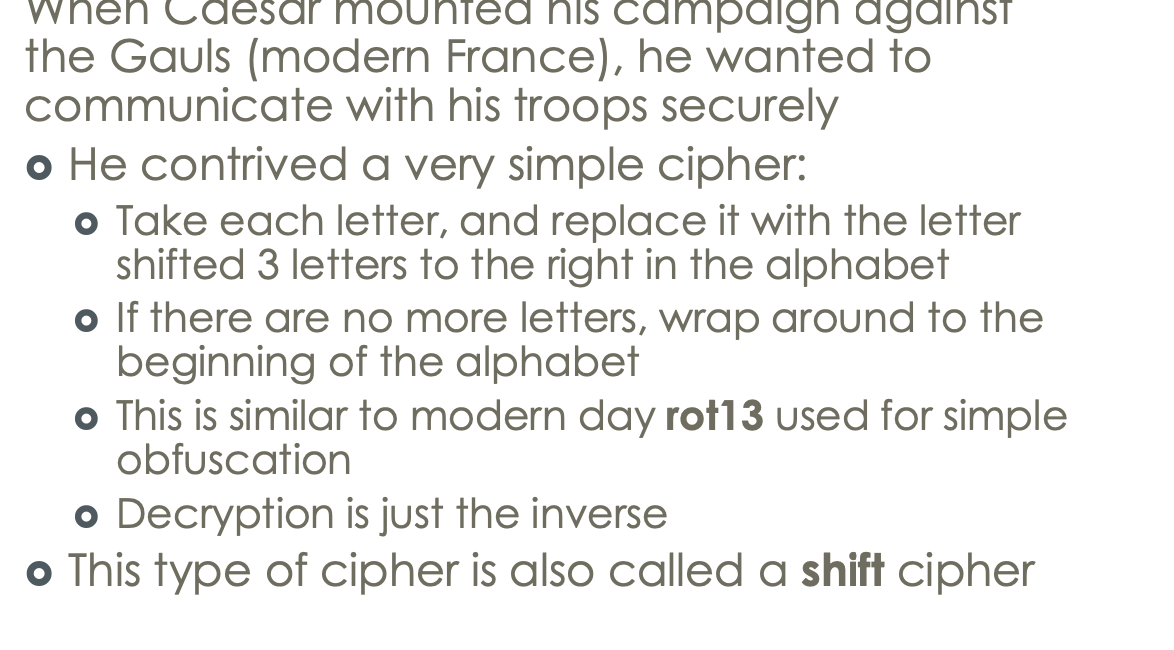
\includegraphics[width=0.8\linewidth]{img/image_2023-01-30-19-13-50.png}
        \caption{A contrived cipher}
    \end{figure}

    Note that even this may be difficult to crack in reasonable time with a brute-force attack if we happen to have a large enough alphabet.
\end{definition}

\begin{definition}
    A slightly better cipher would be a substitution cipher
    \begin{figure}[H]
        \centering
        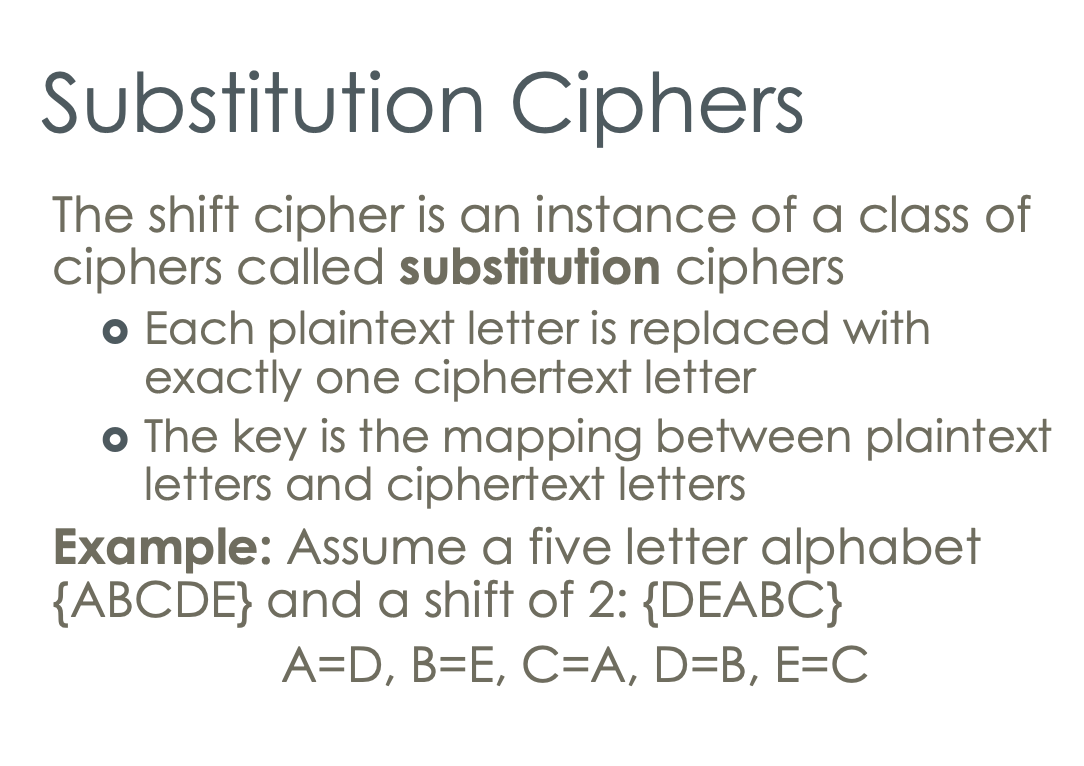
\includegraphics[width=0.8\linewidth]{img/image_2023-01-30-19-21-41.png}
    \end{figure}

    There's a one-to-one mapping between the plaintext and the ciphertext, so we can use patterns in the data to figure out a heuristic to reverse the cipher. For example in English $ E $ is the most common letter (and there are likewise common digraphs e.g. $ TH, HE $, etc) and as such can be used to make informed guesses as to the substitutions being used

\end{definition}

An improvement to the monoalphabetic substitution cipher described above is the polyalphabetic substitution cipher. In this case we have a set of $ n $ mappings in the cipher and change hte mapping with every character.
However these ciphers are still periodic. For small $ n $ this is not a problem, but for large $ n $ it becomes a large challenge.


\begin{blockquote}
    Enigma Machine
    \begin{figure}[H]
        \centering
        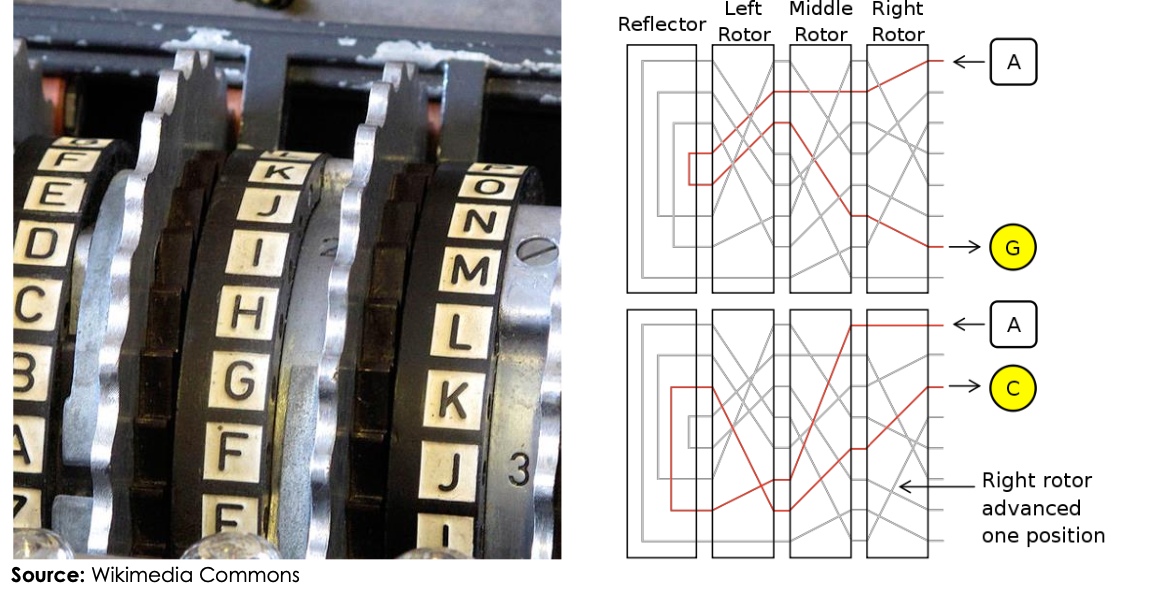
\includegraphics[width=0.8\linewidth]{img/image_2023-01-30-19-30-24.png}
    \end{figure}

    \begin{itemize}
        \item A substitution cipher with a really large cipher during early war efforts
        \item Decryption/encryption via initial rotor position etc that would be agreed on.
    \end{itemize}
\end{blockquote}


The gold standard for encryption is the substitution cipher taken to the extreme: the one-time-pad.

\begin{definition}
    \textbf{One-time-pad}

    \begin{itemize}
        \item A random substitution is used for every character
        \item Think about it as using an infinite number of keys
        \item A message with $ n $ bits of information an OTP adds n bits of randomness to make a completely random ciphertext --> Theoretically unbreakable
        \item Key overhead of 100\% (key length equal to message length) and key reuse is not allowed
        \item Cipher is malleable (bit flips in ciphertext correspond to bit flips in plaintext); requires integrity check
        \item How to make a random key? Need good random number generator
        \item OTP is strong against ciphertext-only attacks but is exteremely weak against known-plaintext attack (only need one pair). 
    \end{itemize}

\end{definition}


Practical ciphers are ones with fixed length keys that are shorter than the message and are independent of message length. They should also be efficient to use for encryption/decryption while being computationally difficult without the key.

\begin{definition}
    Symmetric key ciphers: same key to encrypt/decrpyt (stream/block ciphers)

    \begin{itemize}
        \item Stream ciphers: similar to OTP: key used to generate pseudo-random sequence of bits and then XOR'd with plaintext. Runs a bit at a time which is good for streaming. Suffers from synchronization problems

            \begin{figure}[H]
                \centering
                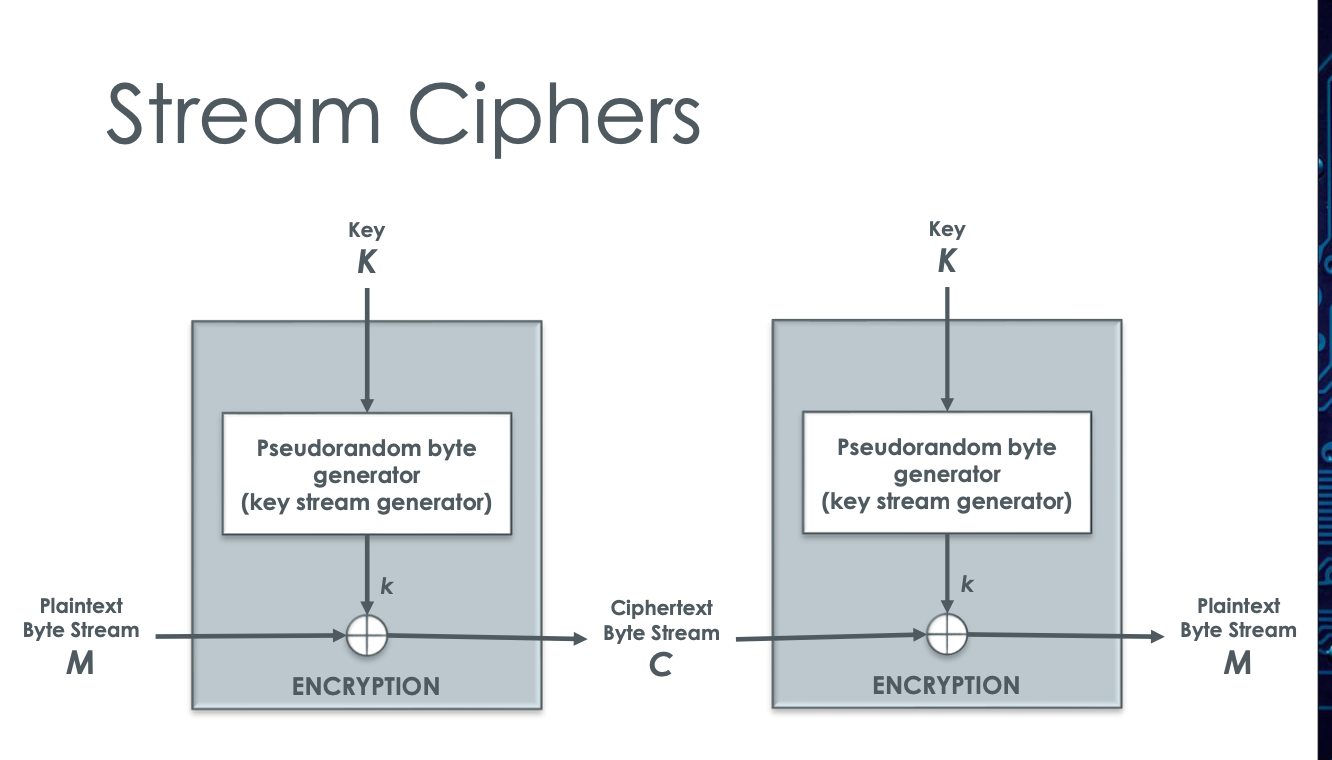
\includegraphics[width=0.8\linewidth]{img/image_2023-01-30-19-43-53.png}
            \end{figure}
        \item Block ciphers: encrypt/decrypt a block of bits at a time (usually 64 bits or a multiple). Add padding if necessary.

            \begin{figure}[H]
                \centering
                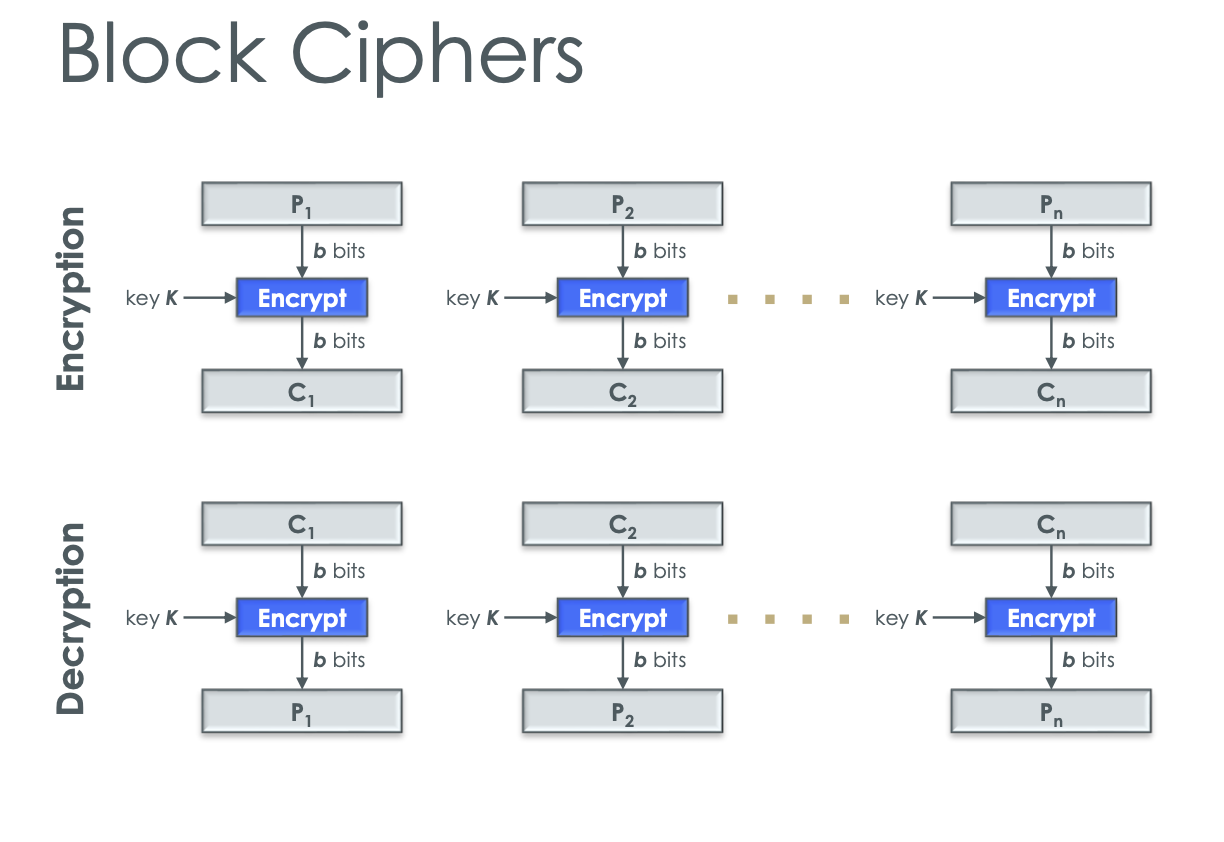
\includegraphics[width=0.8\linewidth]{img/image_2023-01-30-19-44-04.png}
            \end{figure}
    \end{itemize}


\end{definition}

Stream ciphers are generally simple and fast. Block ciphers are more common just due to the history of cipher development (closed-source stream ciphers and a proliferation of open-source block ciphers)


\subsubsection{Block Ciphers}

\begin{itemize}
    \item Data Encryption Standard (DES): 56 bit key, 64 bit block.
    \item AES (Advanced Encryption Standard) -- official standard encryption algorithm for the US government in 2000
    \item Both are iterated block ciphers
    \item Today's computers are fast enough that DES is considered insecure
\end{itemize}


\begin{figure}[H]
    \centering
    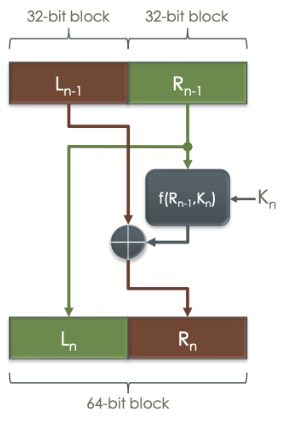
\includegraphics[width=0.8\linewidth]{img/image_2023-02-10-00-07-50.png}
    \caption{DES Feistel Ntwork}
\end{figure}
\begin{itemize}
    \item Input is split between left and right haves. Some computation involving a portion of the key is done on the right half and then the left and right halves are swapped, then the output gets piped back into this process. This "round" is repeated 16 times.
    \item 56 bit key is put through a schedule to create sixteen subkeys. 56-bit into 2 28 bit halves, then shifted left by 1 or 2 bites, and 2 24 bits are then selected from the halves to make a 48 but subkey $ K_n $. Exact number of bit selections are carefully selected.
\end{itemize}

\begin{figure}[H]
    \centering
    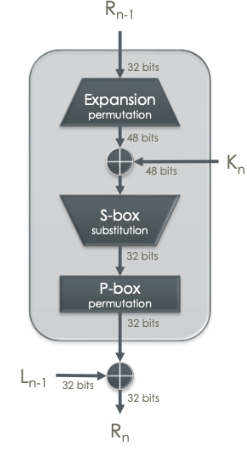
\includegraphics[width=0.8\linewidth]{img/image_2023-02-10-00-10-31.png}
    \caption{each $ f(R_{n-1}, K_n) $ does: 1. expansion permutation 2. XOR with subkey 3. non-linear S-box subsitution boxes to compress 48 to 32 bit 4. permutation}
\end{figure}

\marginnote{Design of S-boxes is important as this is the only part of the cipher that is non-linear}

\begin{itemize}
    \item DES is inadequate with modern computers: brute force can crack 56-bit keys in less than a day. A solution is to use a longer key length and chain DES multiple times; \textbf{3DES} w/ a 168 bit key split into 2 56 bit times and running the algorithm three times
\end{itemize}

\begin{figure}[H]
    \centering
    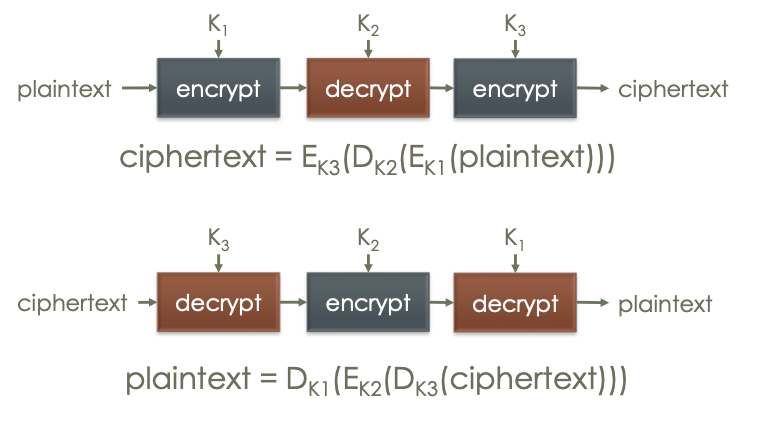
\includegraphics[width=0.8\linewidth]{img/image_2023-02-10-00-19-51.png}
\end{figure}


Block cipher encryption modes, or how to encrypt data with multiple blocks:
\marginnote{Considerations include security, performance, error propagation, and error recovery}

\begin{itemize}
    \item Electronic Cookbook (Simplest): break down into block-sized chunks \& pad if necessary. Encrypt each block separately.
        \begin{itemize}
            \item Highly parallelizable  but not secure
            \item Cipher blocks can reveal macro structure of plaintext data since same plaintext blocks will always encrypt to the same ciphertext blocks
                \begin{figure}[H]
                    \centering
                    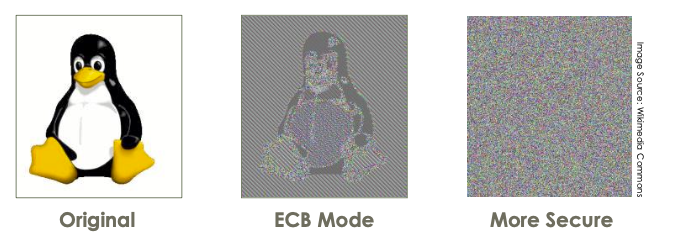
\includegraphics[width=0.8\linewidth]{img/image_2023-02-10-01-29-44.png}
                \end{figure}
            \item Error propagation doesn't happen \& error recovery only requires retransmission of affected blocks and does not stop decryption
        \end{itemize}
    \item Cipher block chaining
        \begin{itemize}
            \item Every block's input is dependent on output of previous block. Initial value does not have to be secret but shouldn't be reused for multiple messages
            \item Good security but poor parallelism for encryption\mn{decryption can be parallelized}. Transmission error only affects current and following block -- and as for recovery the receiver can drop affected blocks and still continue decryption.
        \end{itemize}
    \item CFB (Cipher-feedback) and OFB (Output feedback) convert block ciphers into stream ciphers, i.e. can be decrypted/encrypted in less than a full block at a time. Similar to stream ciphers (Discussed later.) In OFB the key stream is independent of plaintext so cipher operations can be done in advance
\end{itemize}




\subsubsection{Stream Ciphers}

\begin{itemize}
    \item Encryption/decryption with low latency, i.e. multimedia streams
    \item Operate one bit at a time
    \item Closely related to one-time pads
    \item No modes: can be used to encrypt data of any length
    \item Synchronous stream ciphers: key stream is independent of message text. State is modified by $ f $ and the key; each step uses feedback in which $ f $ uses current state to produce the new state. Transmission error only affects the corresponding plaintext bits
        \begin{figure}[H]
            \centering
            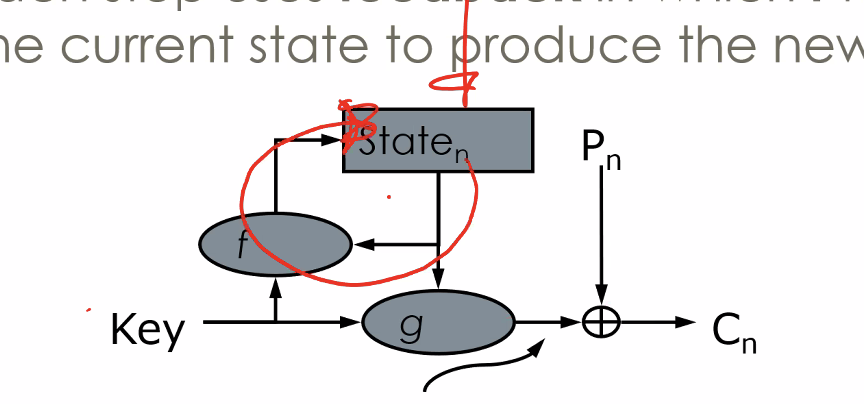
\includegraphics[width=0.8\linewidth]{img/image_2023-02-06-18-43-03.png}
        \end{figure}
    \item Self-synchronizing stream ciphers: key stream is dependent on the plan test. State is a shift register; every ciphertext bit created is shifted into the shift register and fed back as input into the key function $ g $. So each ciphertext bit as an effect on the next $ n $ bits\mn{$ n $ is the length of the shift register}
        \begin{figure}[H]
            \centering
            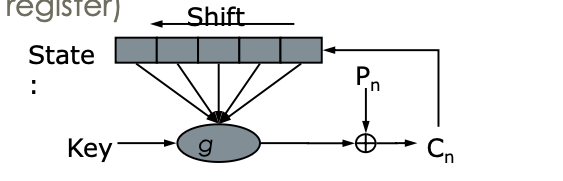
\includegraphics[width=0.8\linewidth]{img/image_2023-02-10-01-39-48.png}
        \end{figure}
    \item Similar properties to the one time pad; dangerous to use the same keystream to encrypt multiple messages
    \item Synchronous stream ciphers must have changed keys or initialization vectors after every message. Self-synchronizing stream ciphers must have random data inserted at the beginning.
    \item Malleable; ciphertext can be changed to generate related plaintext.
    \item Adversaries can replay previously sent ciphertext into a stream and the cipher will resync.
    \item Synchronous stream ciphers cannot be recovered unless we know exactly how much ciphertext is lost because the keystream is independent of the plaintext.
        Self-synchronizing ciphers will recover after $ n $ bits pass.
\end{itemize}

Common ciphers used include RC4 and SEAL. 
RC4 is now publicly known but license is required to use it

\begin{figure}[H]
    \centering
    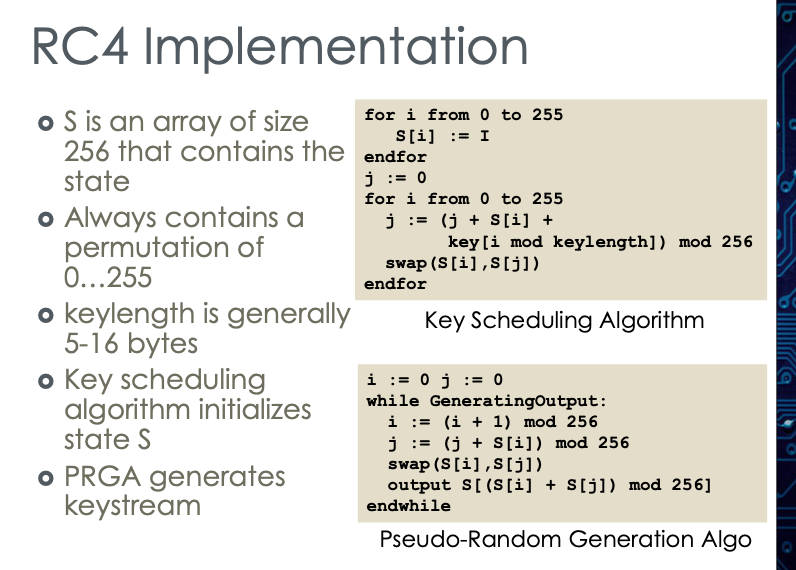
\includegraphics[width=0.8\linewidth]{img/image_2023-02-10-01-42-54.png}
    \caption{RC4 Implementation. TLDR: Use a state represented by an array of 256 chars. Use a pseudo-random generator and the state to generate the keystream.}
\end{figure}


Stream ciphers offer better performance but are more difficult to use safely. Block ciphers are easier and more commonly used. Nowadays just use AES \& CBC is most common encryption mode for arbitrary data. ECB is safe for short chunks of data where plain text is unlikely to repeat.




\subsection{Key Exchange}
\begin{itemize}
    \item Symmetric key encryption requires both parties to have the same key
    \item Key exchange must be communicated securely; if not, the key is compromised
    \item Pre-sharing keys is one alternative; i.e. setting keys at production time. But this is not practical for large systems; $ n $ people need a total of $ n\frac{n-1}{2} $ keys
\end{itemize}

\subsubsection{Trusted third-party}

Idea: have a trusted keyserver that knows everyone's keys.

\begin{figure}[H]
    \centering
    \includegraphics[width=0.8\linewidth]{img/image_2023-02-10-16-43-12.png}
\end{figure}
\begin{itemize}
    \item A tells T that it wants to communicate with B
    \item T sends A a session key $ K_{AB} $ and encrypts it once with A's key ($ (K_{AB})_{K_A} $) and once with B's key
    \item A will decrypt it's own copy of the session key with it's own key and then send the other key to B
    \item B can now decode the session key with it's own key. Now A and B can communicate securely
\end{itemize}

This procedure is susceptible to a third party attacker who may capture the session key $ A $ sends to $ B $ as well as other messages. The attacker can then replay messages to make $ B $ repeat an action; $B  $ can't tell if the message actually came from $ A $


\begin{definition}
    Needham-Schronecker protocol: a protocol for key exchange between two parties $ A $ and $ B $ that is secure against a passive eavesdropper by using a \textbf{nonce} 

    \begin{figure}[H]
        \centering
        \includegraphics[width=0.8\linewidth]{img/image_2023-02-10-16-55-54.png}
    \end{figure}

    \begin{itemize}
        \item Messages include recipient and sender
        \item Receiver keeps track of sent Nonce values to prevent replay attacks
        \item Some action performed on the Nonce proves to the sender that the recipient is alive. Often just adding/subtracting a constant from the nonce\mn{Multiplication or division is discouraged due to the nature of many of these algorithms}
    \end{itemize}

Trusted third party has a problem: because the system trusts the central server, if the server is compromised, the entire system is compromised.

\end{definition}


\subsubsection{Diffie-Hellman Key Exchange}

\begin{itemize}
    \item Can be used by two parties to establish a common secret over an insecure link
    \item Assumes that the discrete logarithm problem is hard (modular arithmetic in a finite field)
        \begin{itemize}
            \item Limited set of $ n>1 $ elements, each with an additive inverse $ x + x' = 0 $ and each nonzero element has a multiplicative inverse $ x \cdot  x' = 1$
            \item Recall: Modular arithmetic is the same as addition and multiplication but with the result rounded by the modulus of $ n $, i.e if our system has a modulus of $  7 $ then $ 4+3 = ((4+3)\%7) = 0$.
            \item There are no negative numbers or factions in modular arithmetic, so additive and multiplicative inverses are as follows:
                \begin{itemize}
                    \item E.x. the additive inverse of $ 4 $ is $ 3 $; $ 4 + 3 = 7 \rightarrow 7 \% 7 = 0 $
                    \item Multiplicative inverse of $ 5 $ is $ 3 $; $ 5 \cdot 3 = 15 \rightarrow 15 \% 7 =  1 $
                \end{itemize}
            \item Modular arithmetic in a finite field will only work if the modulus is prime
        \end{itemize}
    \item  $ 4^3 \% 7 = 64 \% = 1 $, $ \log_4 1 \% 7 = 3 $
    \item What is the discrete log of $ \log_3 5 \% 7 $? I.e. finding $ x $ such that $ 3^x \% 7 = 5 $. Must try all possible values of $ x $ until we find the correct one (and do the exponentiation!).
        \begin{itemize}
            \item Complexity of finding the log is $ NP-hard $
        \end{itemize}
\end{itemize}

\begin{definition}
    Initialization: Alice selects $ n $, a large prime modulus and $ g $, a generator of the field $ n $ that lies between $ (1, n-1) $\marginnote{Generator selection is discussed in texts on the subject. A number $ g $ is a generator of $ n $ if for each $ y $ between $ 1, n-1 $ there exists an $ x $ such that $ g^x \% n = y $, i.e $ g^0, g^1, \ldots g^{n-1}$ yields all numbers from $ 1 \ldots n-1 $}

    \begin{itemize}
        \item Alice selects a random integer $ x $ and computes $ P = g^x \% n $
        \item Alice sends $ P, g, n $ to Bob and keeps $ x $ to herself
        \item Bob selects a random integer $ y $ and computes $ Q = g^y \% n $
        \item Bob sends $ Q $ to Alice and keeps $ y $ to himself
        \item Alice and bob may now both compute the secrete $ Q^x \% n \equiv  P^y \% n \equiv g^{xy} \% n $
    \end{itemize}

\end{definition}

The Diffie-Hellman attack is vulnerable to man-in-the-middle attacks.
If an adversary Eve can pretend to be Bob when communicating with Alice and pretend to be Bob when communication with Alice, then Eve can establish a shared secret with each of them without Alice or Bob being any wiser -- thereby snooping on on their communication!

The problem with this key exchange protocol is that it does not identify the remote party; though the communication is secure we have no clear way of knowing if we are really corresponding with who we think we are.



\subsubsection{Public Key Cryptosystems}
Public key cryptosystems use a pair of keys to establish an asymmetric cryptosystem. The private and public keys reveal nothing about each other, but share the property that messages encrypted with one key can only be decrypted with the other.
Users keep one `private' key secret and one `public' key, well, public. Then during encryption the sender may encrypt the messages with the intended recipient's public key and the recipient can decrypt the message with their private key.
And since only the recipient can decrypt the message, the sender can be sure that the message is only being read by the intended recipient.

Setting up a key exchange using a public key system is straightforward; Alice can encrypt a key $ x $ using Bob's public key and send it to Bob. Bob can then decrypt the key with his private key and now they have a shared key $ x $!
Two popular public key cryptosystems are RSA\mn{Factoring} and DSA (Digital Signature Algorithm)\mn{Discrete logs}



\begin{definition}
    \textbf{RSA} algorithm

    \begin{enumerate}
        \item Pick $ n $ that we can use as basis for the modular space. RSA key generation begins by picking two very large prime numbers $ p $ and $ q $ and computing $ n = p \cdot  q $. $ n $ can be publicky shared since there's no known algorithm to efficiently recover $ p, q $ from $ n $. \mn{Size of $ n $ defines key size; i.e. 4096 bit RSA uses 4096 bits to represent $ n $}
        \item Pick our public key\mn{Via Euler's Theorem}. Define $ \phi = (p-1)(q-1) $. Pick $ e $ that is \textit{coprime}\mn{$ a, b $ are coprime if $ 1 $ is the only positive integer that evenly divides both of them} to $ \phi $; this will be our public key.
        \item  A message $M$ can be encrypted into a cryptotext message $ C $ via $ C = M^e \% n $. $ e, n, C$ can be made public, $ p, q, \phi $ must remain secret. Note that $ M < n $ or else RSA doesn't work.
        \item Calculate our private key, i.e. need a private key $ d $ that is the multiplicative inverse of the public key $ e $: $ e*d = 1 \% \phi $. This $ d $ can be found efficiently through the extended euclidean method\mn{Google this, not needed for the course}. $ d $ must remain private. Also, no-one else can find $ d $ since they don't know $ \phi $.
        \item Recover $ M $ via the private key
            \begin{itemize}
                \item $ M = C^d \% n = (M^e \% n)^d \% n = M^{e \cdot d} \% n $
                \item Since $ e \cdot  d = 1 \% \phi  \Rightarrow (e \cdot  d) = (k \phi + 1) $ for some integer $ k $
                \item $ M^{k \phi + 1} \% n = M^{k \phi} \cdot M \% n = (M^{k\phi \% n } \cdot M \% n) $
                \item Euler's theorem tells us that $ a^{\phi} = 1 \% n $
                \item = $ 1 \cdot M \% n = M $ since $ M < n $
            \end{itemize}
    \end{enumerate}
\end{definition}



RSA has very poor resistance to spoofing since the encryption uses exponentiation; $ encrypt (K \cdot  M) = (K \cdot M)^d = K^d + M^d = encrypt(K) \cdot encrypt(M) $.

Recall that a message is signed by encrypting the message with the sender's private key. The receiver can then decrypt the message using the sender's public key to show that the public key is really yours.
If someone will sign messages the adversary gives them then the adversary can trick them into signing messages that they don't want to sign.
Suppose a victim will not sign $ M $ but the adversary can pick $  K $ and get the victim to sign $ K \cdot  M $ and $ K $. Then $ M $ may be recovered.



Public key cryptography also doesn't prevent man-in-the-middle attacks. If Eve can pretend to be Alice to Bob and pretend to be Bob to Alice, then Eve can snoop without either of them being any the wiser; despite being able to sign a message with one's private key, public key cryptography still suffers from an attacker passing off their public key and signature as someone else's.
This can be resolved through the introduction of a trusted third party who can vouch for the identity of a key.
This trusted third party is called a \textbf{certificate authority} (CA) and they are responsible for issuing certificates using their own private key saying that a public key belongs to a particular person.
Bob and Alice can then use this certificate to verify that they are communicating with the right person.


\begin{itemize}
    \item Common standard format is $ X509 $ and is used in SSL. Public infrastructure allows using a chain of certificates to verify the identity of a key issued by a hierarchy of certificate authorities.
    \item Are we going back to the trusted central server that we were trying to avoid? Yes, sort of. But now the CA is trusted by the public and is not necessarily a single point of failure.
\end{itemize}

An alternative to having a central trusted party is to use $ PGP $; pretty good privacy. This approach builds a web of trust by leveraging the fact that every user is capable of signing certificates and that trust is transitive. If $ A $ can verify that a public key belongs to $ B $, then $ A $ can create a certificate for $ B $ using $ A $'s private key. Then if $ C $ can verify $ A $'s public key then $ C $ can sign a certificate saying so with their private key.

Then we've established a chain of trust from $ C \to  A \to  B$ and so on. If I can trust $ C $ then I can transitively trust $ A  $ and $ B  $ as well. If I trust $ A $ only then I can trust $ B $ but not $ C $. 


This all sounds great until you realize that the web of trust is only as strong as the weakest link. If $ C $ is compromised then the entire web of trust is compromised as well. 
This is why it's important to have the ability to \textbf{revoke} certificates.
Revocation certificates are usually created as a dual to the certificate first created for the public key, and should be stored safely so that an adversary can't falsely issue a revocation. They also shouldn't be self-signed.
Revocation lists are made public and should be referenced when verifying a certificate. If a certificate is revoked then the certificate is no longer valid.





Common techniques when sending messages using public keys include:

\begin{itemize}
    \item To encrypt a message: simply encrypt the message with the recipient's public key.
    \item To prove that a message is coming from you, sign the message with your private key and send the signature along with the message.
    \item To prevent replay attacks, include a nonce (usually just an increasing number) in the message and sign the nonce along with the message.
\end{itemize}


\subsection{Hashes}


\begin{itemize}
    \item A one-way function that converts a large input into a small, typically fixed size output
    \item Low probability of collision; $ H(m) = h $
    \item Can be thought of as a "fingerprint" of the input
    \begin{itemize}
        \item $ m $ is the preimage/input to hash
        \item $ h $ is the hash value or message digest
        \item $ H $ is a lossy compression function
    \end{itemize}
\end{itemize}

A good hash function should have the following properties:
\begin{enumerate}
    \item \textbf{Preimage resistance}: Given $ h $, it should be computationally infeasible to find $ m $ such that $ H(m) = h $
    \item \textbf{Second preimage resistance}: Given $ m $, it should be computationally infeasible to find $ m' $ such that $ H(m) = H(m') $
    \item \textbf{Collision resistance}: It should be computationally infeasible to find $ m, m' $ such that $ H(m) = H(m') $
\end{enumerate}

Assuming that the length of the hash is $ n $ bits, then 

\marginnote{It is also desirable for small changes in the input to result in large changes in the output. }

\begin{itemize}
    \item Second Preimage resistance: $ 2^{n-1} $
    \item Collision resistance: $ 2^{n/2} $ (birthday attack)
\end{itemize}

\marginnote{MDC (modification detection code) is a hash function that is used to detect changes in a message.}

One way to make sure that a message is passed with integrity is to send a hash of the message along a secure channel and then have the receiver recompute the hash and compare it to the one sent. If they are the same then the message was not modified in transit.

\begin{figure}[H]
    \centering
    \includegraphics[width=0.8\linewidth]{img/image_2023-02-13-18-39-54.png}
\end{figure}

If confidentiality is required the communicators may want to encrypt the message.


\begin{figure}[H]
    \centering
    \includegraphics[width=0.8\linewidth]{img/image_2023-02-13-18-41-31.png}
    \caption{Combining MDC with encryption to ensure integrity and confidentiality}
\end{figure}

Nowadays just use SHA256 (SHA2)\mn{MD5 and SHA1 are deprecated}.



\begin{definition}
    \textbf{MAC}: A message authentication code uses a hash to provide integrity and authentication.

    A MAC is constructed as $ h = H(k, M) $ where $ k $ is the secret key and $ M $ the message. The receiver knows that whoever generated the MAC must also know the key, thus authenticating the message source.
\end{definition}


MACs are often constructed from symmetric ciphers.


\begin{figure}[H]
    \centering
    \includegraphics[width=0.8\linewidth]{img/image_2023-02-13-19-10-15.png}
    \caption{CBC-MAC}
\end{figure}

This method is similar to CBC encryption for block ciphers except a single hash value is produced at the end. Hash size is the same as the block size of the block cipher.
The MAC key must also be different from the encryption key\mn{This is bad practice and can produce a vulnerability depending on your encryption schemes and their interactions}.

A MAC can be constructed by concatenating the secret key with the message and using a mash, which creates a keyed-hash MAC (HMAC)

\begin{figure}[H]
    \centering
    \includegraphics[width=0.8\linewidth]{img/image_2023-02-13-19-14-44.png}
    \caption{HMAC creation}
\end{figure}

An inner and outer hash gets rid of the extension problem since this requires the inner hash to be extended as well (which is encrypted!).
HMACs are a reliable way to give strong signatures to messages.






\begin{figure}[H]
    \centering
    \includegraphics[width=0.8\linewidth]{img/image_2023-02-13-19-18-04.png}
    \caption{HMAC process (opad and ipad are flipped here relative to RFC 6328)}
\end{figure}


\subsubsection{Hash-based data structures}

\begin{itemize}
    \item It is often useful nowadays to have a data structure that can be updated in a secure way and to verify the integrity of a set of things instead of a single object.
\end{itemize}

\begin{figure}[H]
    \centering
    \includegraphics[width=0.8\linewidth]{img/image_2023-02-13-19-23-05.png}
    \caption{Merkle Tree}
\end{figure}

\begin{blockquote}
   Consider we have a bunch of data that we want to keep track of (Data blocks, lowest level of tree in diagram). We can hash all of them and then build a binary tree from the bottom up of the hashes. A parent of two nodes will take on the hash value of the concatenated hash of the it's children. And then the root node would have the hash of everything. The reason why this is better than concatenating all the data blocks and then hashing it together is that the individual blocks we're hashing is a lot smaller and changing a block won't require rehashing along the entire set of data blocks; you will only have to hash $ \log_2 n $ times; from the data block up to the root. 
   The top hash is a hash of all the data blocks and can be used to verify the integrity of all the data we're looking at.

\end{blockquote}


\subsection{Attacks on protocols}

\subsubsection{Replay Attack}

Suppose an attacker Calvin cannot create valid messages but they can record messages between Alice and Bob. If no replay protection is used, Calvin can simply replay the messages to Bob and pretend to be Alice. 
For example consider a wireless deadbolt lock. If the lock is not protected against replay attacks, Calvin can simply record the messages between Alice and Bob and replay them to Bob to unlock the door.
A common way to prevent replay attacks is to use a nonce; an unique one-time value appended to a message.A nonce is an unique value\mn{Random numbers are often used but it is usually preferable to simply use an incrementing counter as to avoid the client on having to store a ton of nonce values. Also, it's usually a bad idea to use time for nonce values; leap seconds exist and time is tricky.} 
\begin{figure}[H]
    \centering
    \includegraphics[width=0.8\linewidth]{img/image_2023-03-12-19-00-40.png}
    \caption{Appending message with a nonce to prevent replay attacks. It's important that the hash value and message are both encrypted or included with the hash.}
\end{figure}

Counter also help prevent reordering attacks. An example of where a reordering attack can be dangerous is if we're controlling a drone; going forwards 10m and then to the right 10m is a different trajectory than going right 10m and then 10m forwards.
One thing to note is that packets can arrive out of order which means that the nonce value may not come in the correct order -- so you need to keep track of the nonce values you've seen before. This is called a nonce cache.



\subsubsection{SSL}

The SSL protocol is a protocol for secure communication over the internet commonly used to secure web sessions\mn{And can be used to secure any application since it operates on regular sockets}.
It is implemented as an application level library and is linked with both the client and the server. 
It presents the same functionality as a socket but it encrypts the data before sending it and decrypts the data before receiving it -- the network doesn't need to have any security (i.e. SSL provides end to end security)

\begin{figure}[H]
    \centering
    \includegraphics[width=0.8\linewidth]{img/image_2023-03-12-19-11-33.png}
\end{figure}


SSL includes two phases:

\begin{enumerate}
    \item Key exchange/handshake: checks versions, sets up secret key \& does auth. Only happens once, so it can be slow
        \begin{itemize}
            \item Establishes the ciphers each side supports and the version of the protocol. Establishes a shared secret key (session key). Authenticates each other's identifies via certificates. Note that this authenticates the machines and not the users. User auth is usually done by the web server. Nte that client auth is optional and not done for every SSL interaction since web servers generally connect to any client.
        \end{itemize}
    \item Communication: encrypts and decrypts data. Happens for every message. Needs to be efficient.
\end{enumerate}


\begin{blockquote}
    You should keep your OpenSSL version up to date since there are known vulnerabilities in older versions and new vulnerabilities are discovered all the time.
\end{blockquote}



\begin{figure}[H]
    \centering
    \includegraphics[width=0.8\linewidth]{img/image_2023-03-12-19-26-10.png}
    \caption{Note that the client hello is sent in plaintext, which means that a man in the middle can alter the list of ciphers it supports -- a downgrade attack. If the server is OK with any cipher then a man-in-the-middle could easily force it to pick an old and broken cipher -- which motivates the server picking the cipher. This step of the handshake is entirely completed in plaintext.}
\end{figure}





\begin{figure}[H]
    \centering
    \includegraphics[width=0.8\linewidth]{img/image_2023-03-12-19-40-24.png}
    \caption{ The next step is the key exchange. This may look a little bit like our diffie-hellman section, at least in our goal to produce a shared secret in a secure manner. All following communication is then performed securely using that shared secret. }
\end{figure}

This handshake protects against: 1. spoofing via MAC, 2. reordering protection (nonce), 3. replay (nonce), 4. man-in-the-middle (certificate).


\begin{figure}[H]
    \centering
    \includegraphics[width=0.8\linewidth]{img/image_2023-03-12-19-42-16.png}
    \caption{Once we go into communication mode SSL has a few more tricks to protect against attacks. Note that compression is somewhat controversial since it can be used to leak information about the data being sent.}
\end{figure}

SSL generally doesn't impose much performance penalty on the actual communication layer since it's only encrypting and decrypting the data using a fairly fast symmetric block cipher. 
However the serbver uses asymmetric decryption during handshake (which is about 1000x times slower than symmetric decryption). This means that for servers with a lot of SSL work to do are bottlenecked by the handshake.\mn{Consider situation when a server goes down and then a stampeding herd\mn{sort of?} of clients try to reconnect.}
Dedicated hardware does exist to perform public key operations to speed up the handshake process.
From a system architecture perspective it is common to set up servers in such a way for them to operate directly on cleartext and have a seperate SSL proxy server that handles the outside world.


\subsubsection{SSL Demo}





Here are some steps for setting up a web server and to create a certificate for it:


\begin{listing}[H]
\begin{minted}{bash}
# we need to trust someone at first. With public key auth. we just need to trust that the certificate authority is giving keys to the right people.
# We can also be our own certificate authority!

#  request a new x509 certificate (cakey.pem)
# - v3_ca tells it that this is a certificate authority
# - give it a timeout and want 4096 bit key
openssl req -new -x509 -extensions v3_ca -keyout cakey.pem -out cacert.pem -days 3650 -newkey rsa:4096

# follow through with the prompts & optionally give the PEM a passphrase.
# can read the keys with: (note this will prompt for passphrase)
openssl rsa -in cakey.pem -text 

# can read the certificate with:
openssl x509 -in cacert.pem -text 

# now let's make a key pair for our web server

openssl genrsa -des3 -out server.key 2048

# as the server let's request a certificate for our public key
# from our CA; create a csr (certificate signing request)
openssl req -new -key server.key -out server.csr


# now we can sign the certificate for a year with our CA
# serial is for keeping track of the certificates that we've signed
openssl x509 -req -days 365 -in server.csr -CA cacert.pem -CAkey cakey.pem -CAserial serial.txt -CAcreateserial -out server.crt

# now we've created server.crt which is the certificate that we'll give to the client to prove that the server is who it says it is, at least according to the CA

\end{minted}
\end{listing}


Let's say we try to run a server with this certificate. The client, a web browser, will check the certificate to see if it is from a CA that it trusts. Unfortunately the CA we just isn't trusted (i.e. not in the client's trust keychain) so it won't be immediately useful for web serving.
A use case where we may want a self-signed CA is if a company wanted to monitor all internet traffic for their employees. They could set up a proxy server that intercepts all traffic and then they could set up a CA and sign all of their employees' certificates. 
And then add the CA's certificate to the trust keychain of all of their employees' computers. This way the employees' computers will trust the CA and will trust the certificates that the CA signs -- so the employees can access the internet as if everything is trusted by the company may watch the traffic and make sure that employees don't leak credit card information or something.

In practice most CAs will have one top level key stored in an absurdly secure location and then they will have a bunch of subordinate keys that are used to sign certificates. The subordinate keys are stored in a secure location and the top level key is used to sign the subordinate keys. This way they can easily rescind subordinate keys if they get breached.


\subsubsection{Web Authentication}

It is impractical to require all users to use a certificate to identify themselves -- hence username/passwords.


\begin{definition}
    Cookie-based authentication


    \begin{enumerate}
        \item Browser asks for username and password and gives it to the server
        \item On auth server generates a big random-looking number called a \textbf{HTTP cookie} and returns to the browser
        \item Next time the browser visits the same server it will send the same cookie back to the server: the cookie is used as an authentication token
        \item Web servers use cookies to authenticate the user as well as store session information, etc.\mn{If a cookie can be stolen before it expires it can be used to impersonate the user}
        \item Should have a expiry time (limits damage from exposed cookies) and be as ephemeral as possible
        \item Should be hard to forge a cookie and should not be used for authentication without SSL (or else they are easily stolen)
    \end{enumerate}

    A drawback of cookies is that they can raise privacy concerns; web servers can now track users' browsing habits within a site as well as across sites as well.
    
\end{definition}

\marginnote{Recall: GET is used to read data from a server and POST is used to update data on a server. The line has been somewhat blurred in recent years.
}

Browser-based attacks are common and usually performed via some sort of cleverly formatted GET or POST requests to the server (with XSS).

A GET request contains a header, a blank line, and the content. The POST is almost the same, except it requires a few more header fields to specify the content type and length.


It is very common for sites to have web browsers execute small javascript programs, i.e. some logic to run \texttt{onclick} when a button is clicked.
One way to exploit this is possibly to find a way to make the browser think that data is actually a program -- like buffer overflow attacks!


\marginnote{\href{browserspy.dk}{browserspy.dk} is a website that shows you how much information your browser is leaking to websites.}



Javascript can be used to read and steal data
\begin{itemize}
    \item Cookies can be read by JS by accessing the \texttt{document.cookie} variable
    \item Script can incorporate the cookie data into a request to the attacker server and send it back
    \item Protected via the \textbf{Same Origin Policy}: dictates that scripts from one origin (a web site) cannot access or set the properties of a document from another origin/website. 
    \item URLs are treated as having the same origin if they are on the same protocol, hostname, and port number.. Browser isolates different sites into different identities. Note that domains under the control of the same organization, i.e. google.ca or google.com are not considered the same origin
\end{itemize}

Many sites include javascript from third-party sources, i.e. from ad networks. This opens up the possibility of cross-site scripting attacks.

\begin{definition}
    Cross-site scripting (XSS) is a vulnerability that allows a user to inject strip code into web pages viewed by other users. Allow for stealing cookies of a victom web site and more.

    \begin{enumerate}
        \item  Type 1/reflected: Attacker crafts url that targets a vulnerable site, attacker needs to click on url for a successful attack, web site is not modified
        \item   Type 2/Persistent: Attacker posts malicious code on a vulnerable site, users must visit the site to be affected, web site is modified
    \end{enumerate}
\end{definition}



\begin{figure}[H]
    \centering
    \includegraphics[width=0.8\linewidth]{img/image_2023-03-12-21-31-07.png}
    \caption{What if some code is given to the browser to the browser instead of the name? I.e. as in the next slide?}
\end{figure}


\begin{figure}[H]
    \centering
    \includegraphics[width=0.8\linewidth]{img/image_2023-03-12-21-32-01.png}
    \caption{The victim website will execute the code and send the user's cookies to the attacker. By bouncing (reflecting) it off the server it looks like code that doesn't violate the same origin policy.}
\end{figure}


Generally XSS is a result of poor input validation.



\begin{blockquote}
Persistent XSS: Many sites want users to post their own content, which has conflicting requirements. They want to give users the ability to post rich content but also want to make sure that they don't post content that harms other users (XSS). Most sites will perform input validation (filtering) on user posts to remove code but still allow users to post rich content.
\end{blockquote}




Defenses against XSS

\begin{itemize}
    \item Convert all special characters before sending to an user, i.e. "<" -> "\&lt;a"
    \item Whitelist characters (don't just blacklist -- too many characters to blacklist)
    \item Use HTTP-only cookies (cookies that can't be accessed by javascript). This has the downside of limiting the functionality of the site.
\end{itemize}



\subsubsection{SQL Injection}
Consider an insecure web application that allows users to look up their information by their USER ID
\begin{figure}[H]
    \centering
    \includegraphics[width=0.8\linewidth]{img/image_2023-03-13-18-49-22.png}
\end{figure}

This may form a SQL query like this

\begin{listing}[H]
\begin{minted}{sql}
select id, first, last from users where id = '%s'
\end{minted}
\end{listing}

Is there a way for us to exploit the server not checking for apostrophes in the query? Consider the following query


We insert \texttt{1' and 1 = 1 -- '}



\begin{listing}[H]
\begin{minted}{sql}
select id, first, last from users where id = '1' and 1 = 1 --' 
-- Note that -- is a comment to make this valid sql
\end{minted}
\end{listing}

And we find that this query ends up returning the user 1! And it is easy to see how this can be extended to get the information of every user by extending the query with an \texttt{or}.


What about some more complex queries? For example some databases can load a file with the \texttt{load\_file}. So this would give the \texttt{passwd} file for the database server.


\begin{listing}[H]
\begin{minted}{sql}
select id, first, last from users where id = '1' union select load_file('/etc/passwd'), 'foo' --'
-- And whatever we want in foo..
\end{minted}
\end{listing}


Other ideas include

\begin{listing}[H]
\begin{minted}{sql}
-- the schema
' union select table\_schema, table\_name from information\_schema.tables --' 

-- users and apasswords
' union select user, password from dvwa.users -- 

\end{minted}
\end{listing}




Note that this, on any decent web service, will return a bunch of password hashes.
Fortunately most users suck at picking passwords and so we can use a rainbow table to crack the hashes, i.e. by using hashcat;

\texttt{hashcat <file\_with\_password\_hashes> /var/pentest/wordlists/top\_100\_passwords.txt}

\marginnote{
    We should consider the implications of this. For example the \texttt{load\_file} attack would not be possible if we ran the sql server as a non-root server or as an user with restricted access.
}

\subsubsection{Passwords}

Passwords are commonly used for user authentication but have several problems:
\begin{itemize}
    \item Users tend to pick easy passwords and share them for many systems
    \item Authentication is not mutual: when a user enters a password they usually don't know if they are sending the password to the right system
\end{itemize}

Passwords should not be stored in the clear so that if the attacker somehow got the password file they would know the passwords of all users -- so passwords are hashed with a one-way hash and only the hash is stored.
However if the attacker reverses one password hash then the attacker will have found the password for all users using the same password (not uncommon!). This problem can be prevented by adding a salt (some random value concatenated with the password) which is stored alongside the password file. This doesn't make it more or less difficult to break a single password because the number of password bits still remain the same (instead of guessing h(<password>) they now guess h(salt + <password>) but salt is known).




\subsubsection{HTTP Response Splitting}


HTTP response splitting is a vulnerability that takes advantage of the fact that HTTP naively parses requests to split it into a header and a body just by looking for a carriage return and line feed sequence. 
If the string \texttt{English} is user input, an attacker can send a request with the language set to \texttt{English\\r\\n  ...} and the server will interpret this as a header and a body. The attacker can then send a response that will be interpreted by the browser as a header and a body. This can be used to inject malicious code into the response.

\begin{blockquote}
    This is something that has largely been dealt with but sometimes still pops up in legacy or embedded systems.
\end{blockquote}





\subsubsection{Cross-Site Request Forgery (CSRF)}

\begin{blockquote}
    This one is still relevant and is a common attack vector.
\end{blockquote}

A vulnerability that allows unauthorized commands to be executed on a web application from an user. Tricks users into visiting a website that contains a link to a site that the user may have visited previously.
If the user's browser contains a valid authenticated cookie for the site, the attacker can issue authenticated requests to the site.


For example, 

\begin{listing}[H]
\begin{minted}{html}
<img src="http://bank.com/transfer?amount=1000&to=attacker"
\end{minted}
\end{listing}

This would simulate a user visiting the bank's website and transferring money to the attacker via the request. There's technically nothing wrong with it because the request is coming from the user's browser. But the user didn't intend to do this.
It also doesn't violate the same origin policy because it doesn't involve requesting for cookie contents.

This is very difficult to fix on the client side and largely would have to be kept in mind by the application developer\mn{This is why banks tend to have layers of confirmation screens and short authentication lifetimes.}.


Defenses against CSRF:

\begin{itemize}
    \item Limiting the lifetime of authentication cookies
    \item Checking HTTP referrer headers (make sure that the referrer is the URL of the previous webpage from which a link was followed) (but this can be possibly forged, depending on the browser)
    \item Requiring secret token in the GET and POST parameters
    \item Requiring authentication in GET and POST parameters, not in cookies only
\end{itemize}



\subsubsection{Multi-Factor Authentication (MFA)}

\begin{itemize}
    \item Authentication, in general, uses a piece of information about the user (authentication factor) to verify that the user is who they say they are. This is usually something that they know, they have, they are, or can do.
    \item Multi-factor authentication is a method of authentication that requires more than one authentication factor to be used to verify the user.
        \begin{itemize}
            \item For example: smart credit cards contain a secure chip that can be used to authenticate the user that contains keys and performs cryptographic operations, usually having the card sign a randomly generated string
            \item As discussed in the labs, the user can also use a one-time password (OTP) that is generated by a hardware token or a mobile app
            \item Biometric systems:
                \begin{itemize}
                    \item Moving from binary to probabilistic security model (false rejection/false acceptance)
                    \item Layered approaches and good management of biometric templates are necessary
                \end{itemize}
        \end{itemize}
\end{itemize}


\subsubsection{Federated Identity}

A single service maintains a user's username and passwords. Handles new registrations, password resets, etc. Multiple services rely on the identity provider to help authenticate users that interact with the services. UTORid is an example.

A case study is the Kerberos system, which is a federated identity system that is used by many organizations to authenticate users via a trusted third party and Needham-Schroeder. The trusted third party uses an authentication server and a ticket-granting server.



There are three layers to it:
\begin{enumerate}
    \item Authentication
    \item Authorization
    \item Service
\end{enumerate}
\begin{figure}[H]
    \centering
    \includegraphics[width=0.8\linewidth]{img/image_2023-03-13-20-50-25.png}
\end{figure}

The authentication layer creates a secure token given to the user that the user can then use to prove that they are why they claim they are.
Next, they go through the authorization server using it's token to get a service token. This authorization service has no idea how to authenticate but it can know if the key is valid. This token is then used to access the service, i.e. printing.
The service can then use the ticket to grant access to whatever the ticket is for.


\begin{blockquote}
    A nice part of this kind of layered system is that it offers flexibility and agility in design and maintenance. This is especially important for a changing product.
\end{blockquote}




\begin{definition}
    Single-sign-on (SSO): enables a user to log in once and access multiple services without having to log in again. Generally implemented through some sort of federated identity protocol.
\end{definition}


Typical web authentication flow:

\begin{enumerate}
    \item User authenticates to the identity service provider
    \item Service provider sends the user an \textbf{unforgeable}  token
    \item User presents token to service they want to access which it accepts n lieu of authenticating the user
    \item The service now has a certified identity for the user
\end{enumerate}


\begin{example}
    \textbf{OAuth}:  An open specification developed by google and facebook for an authorization protocol that is often used as an authentication protocol.

    There are three parties involved:
    \begin{itemize}
        \item \textbf{Resource Owner}: the user. A way to think of this is that you are the profile owner.
        \item \textbf{Authorization Server}: the service that the user wants to access
        \item \textbf{Client}: the service that the user wants to access
    \end{itemize}

    \begin{figure}[H]
        \centering
        \includegraphics[width=0.8\linewidth]{img/image_2023-03-27-20-56-02.png}
    \end{figure}

    The service that we want to access (client) will send a request to us (resource owner) when we want to log in. The user will then use our information and that client request against the authorization server in order to obtain an auth code. The same person who logged in also is the one who hands it back to the client, who uses the authorization server in order to validate things and access the requested information.
\end{example}

Federated identity takes a lot of the security burden off the developer which has significant productivity benefits.
\marginnote{Note: understand difference and relationship between authorization and authentication. Revocation is ok for authorization but is tricky for authentication}





\subsection{Security Modes and Covert Channels}



\subsubsection{Security Policies}
Security policies govern how a system handles information. They are generally used by the military/government/etc. and are based on security models that are usually fairly intuitive but can also stand up to proofs for security. They are generally implemented as MAC\mn{Mandatory Access Control} policies.


\begin{itemize}
    \item Confidentiality Policies: defines who is allowed access information or resources (protect information from leaking)
    \item Integrity Policies: prevents corruption of information
\end{itemize}


\begin{definition}
    Bell-La Padula (BLP) Model: a model designed to build confidentiality policies.
    The idea behind BLP models is that it defines certain levels of data, i.e. unclassified, classified, secret, top-secret, and so forth.
    And each level will be able a file up to a certain level but cannot write \textit{down} to another level.

\end{definition}

BLP does not preserve any integrity, however.

\begin{definition}
    Biba Integrity Model: the mathematical dual of the BLP model, designed to build integrity policies.
    Consider a research experiment that flows from lab measurements -> report -> peer review -> media -> twitter. Then we allow an \textit{write-down} policy to be implemented; there's no danger to the data if we write a twitter post using the media, but there is definitely danger to the data's integrity if we use a twitter post to generate lab measurement data.
\end{definition}





\subsubsection{Side channels and Covert Channels}

\begin{definition}
    A side-channel allows for unintentional information flow in or out of the system, e.g. user data or cryptographic keys.
    Channels can come in many unexpected forms, i.e. R/F leakage, event timing, etc.
    While some side channels can be remotely exploited, many more can be exploited locally.
\end{definition}

Timing analysis is one side channel that relies on the fact that algorithms can somethings leak important security information.
For example, standard \texttt{strcmp} implementations will short circuit at the first character that is not equal -- so the runtime of the method is proportionate to the number of \textit{matching} characters.
So by feeding in a ton of test strings and carefully inspecting the timing we may be able to discover how close we are to the correct string.

\begin{figure}[H]
    \centering
    \includegraphics[width=0.8\linewidth]{img/image_2023-03-28-15-37-17.png}
\end{figure}

Modern cryptographic libraries have fallen victim to timing attacks before. A general recommendation is to add some randomness to the runtime of any cryptographic routine with runtime related to the input.

\begin{figure}[H]
    \centering
    \includegraphics[width=0.8\linewidth]{img/image_2023-03-28-15-44-01.png}
    \caption{Radio emissions from scan patterns of old CRT monitors can be used to reconstruct the image. This is still possible with modern LCD screens, albeit weaker.}
\end{figure}

A similar principle applies to input devices such as keyboards and mice. Wireless keyboards often transmit the input text in plaintext, and wired keyboards need some sort of decoding circuit that will still nonetheless leak the data.


Power analysis is another side channel that can be used to extract information from a system.
For example many safes with electronic locks will want to avoid putting their power source in the safe (so that you don't end up losing access if the batteries run out). This, however, leaves the power consumption of the circuit open for the attacker to observe.

\begin{figure}[H]
    \centering
    \includegraphics[width=0.8\linewidth]{img/image_2023-03-28-15-49-15.png}
    \caption{A voltmeter can be put between the battery and the circuit to measure the power consumption.}
\end{figure}


\begin{figure}[H]
    \centering
    \includegraphics[width=0.8\linewidth]{img/image_2023-03-28-15-51-23.png}
    \caption{In this case we have physical access to the device. So we can connect a probe to the memory chip and monitor the signal with an oscilloscope. The top line is the clock signal and the bottom is the power}
\end{figure}

A clear correlation appears between the power consumption and the clock signal. EEPROMs are quite power hungry, especially when pushing out an 1. 

\begin{figure}[H]
    \centering
    \includegraphics[width=0.8\linewidth]{img/image_2023-03-28-15-53-12.png}
    \caption{As it turns out whenever we enter any combination the EEPROM will wake up the chip and read out the actual stored password.}
\end{figure}


Current research in the field of power analysis includes building chips that inherently have random noise in their power consumption, applying machine learning to better filter out noise, and running chips with inconsistent clock signals and voltage dithering.


\begin{definition}
    Covert channels are much the same as side channels, but they are intentionally designed to leak information.
    There are some pretty crazy ones e.g. setting the speed of a fan, or flipping the Ethernet settings on a raspberry pi to send off a radio signal, etc.
    Covert channels are generally very hard to detect, but there are ways to prevent creating the opportunity for them to exist in the first place.
    Since convert channels exist when the actions of one process affect the actions of another process in a predictable way (even though there is no explicit communication), we aim to design systems with the \textbf{non-interference} property, i.e. any sequence of inputs to a process will produce the same output regardless of inputs to another process\mn{This is almost impossible to achieve in practice}.
    For example a machine should respond the same way to an user with low or high clearance.
\end{definition}

Note that not all covert channels are useful. If you can only get one bit per hour out of a covert channel, it may not be of any practical use to an attacker.






\subsection{Network Security}



\begin{figure}[H]
    \centering
    \includegraphics[width=0.8\linewidth]{img/image_2023-03-28-16-30-18.png}
    \caption{Some key protocols of the internet. 1. ARP is used to map IP addresses to MAC addresses (which is an unique address for each network card) and is at the lowest level. 2. ICMP is a routing protocol, 3. TCP/IP routes packets, and so forth.}
\end{figure}



\begin{figure}[H]
    \centering
    \includegraphics[width=0.8\linewidth]{img/image_2023-03-28-16-31-56.png}
    \caption{Each layer of the network stack adds some header or footer to the packet, but they don't apply any security protocols to it; they just directly trust it.}
\end{figure}

Many of our internet protocols were designed assuming that the network was a trusted environment. For example \texttt{smtp}\mn{for email} just sends everything in plaintext.


\subsubsection{ARP spoofing}

ARP is used to map IP addresses to MAC addresses such that IP packets can be sent to the link layer. Packets are set to the next hop using MAC addresses. 
ARP uses broadcasting: if a host wants to send a packet to address A, then it will perform an ARP broadcast to determine which devices owns IP address A. All hosts ignore the broadcast except for A, which will respond with its MAC address. Then all packets sent to A are sent using the provided MAC address.

If an attacker has full access to a host, then spoofing ARP requests is trivial. The attacker can make all traffic redirect to itself by responding to all ARP broadcasts (every machine starts to think that the hacked machine owns every IP address). \mn{ARP broadcasts are never forwarded outside of a subnet so the attacker must control a machine on a subnet}
Furthermore, on basically every single system the networking stack will opportunistically cache ARP replies and poison\mn{Put incorrect entries in} their own cache.
Then future transmissions from the victim will be routed towards the attacker\mn{To keep this up, the attacker should keep track of who used to own the address and then forward it onwards after relabelling to the old MAC address}

\subsubsection{ICMP Smurf attack}

\begin{figure}[H]
    \centering
    \includegraphics[width=0.8\linewidth]{img/image_2023-03-28-16-47-45.png}
    \caption{Smurf Attack}
\end{figure}

Smurf attacks are a type of reflected attack where we trick a whole host of, well, hosts to all send ping replies to a victim machine. So the attacker sends a ping stream to an IP broadcast address with a spoofed return address.
In the past UofT's network was sensitive to this but (unfortunately?) it is no longer the case.
Defenses to this attack include disabling the host response to ping broadcast, or disabling broadcast forwarding at the router.

\subsubsection{TCP/IP Spoofing}

\begin{figure}[H]
    \centering
    \includegraphics[width=0.8\linewidth]{img/image_2023-03-28-16-54-17.png}
    \caption{TCP Handshake: An attempt is made to make sure that the client is alive}
\end{figure}

\marginnote{According to the standard the SYN and ACK packets should be sent separately but everyone sends them as one}

The TCP handshake uses the initial sequence numbers as a weak authenticator. However, since it is sent in plaintext, an attacker can forge a packet with the source IP address set to the client's address.
Forging source IP addresses don't necessarily allow for the attacker to receive packets directly, but if the attacker can guess the sequence number then the attacker can connect to the server as the victim client.


\subsubsection{TCP Reset Attack}
A reset packet is sent when a server/client want to terminate their connection. This is abused by an attacker by falsely sending reset packets\mn{Often done by listening over the network to find the TCP sequence numbers} to produce a denial of service attack. 
Unfortunately defenses are not obvious and may include ignoring bogus reset packets or requiring multiple packets.

\subsubsection{TCP SYN Flood}
\begin{blockquote}
    The high-tech equivalent of running a doorbell and running away.
\end{blockquote}

The attacker sends a lot of connection requests with spoofed IP source addresses. The victim will allocate resources to handle these requests until some limit is reached, leading to a denial of service.
Defenses include rate limiting, or using a SYN cookie\mn{This breaks the TCP handshake protocol a bit but it provides more defense against such attacks}.

\begin{figure}[H]
    \centering
    \includegraphics[width=0.8\linewidth]{img/image_2023-03-28-17-02-16.png}
\end{figure}


Low-powered firewalls i.e. in embedded systems may only filter the first syn packets. Syn-ack cookies can pose a problem for them since our network flow may establish a connection much further down from the initial syn packet. Many modern communication protocols do take advantage of syn-ack cookies and break the TCP/IP standard in doing so, so this is something to watch out for.



\subsubsection{BGP: Border-Gateway Protocol}

The internet is broken up into autonomous systems (AS) that are independently managed and connect to each other via gateways\mn{I.e. an ISP}. 
Gateways communicate via BGP to update routing information to handle scenarios such as a router going down. This is performed in a peer-to-peer manner.

\begin{figure}[H]
    \centering
    \includegraphics[width=0.8\linewidth]{img/image_2023-03-29-14-57-31.png}
\end{figure}

Routers trust each other and don't authenticate advertised routes or BGP packets.
Therefore BGP can be compromised in a manner similar to ARP attacks, i.e.if a malicious actor gains access to a network it can advertise "good" routes that actually route to the attacker's gateway instead of the intended ones.


\subsubsection{DNS}


\begin{definition}
    DNS (Domain Name System) is a hierarchical system for resolving symbolic names to IP addresses.

    \begin{figure}[H]
        \centering
        \includegraphics[width=0.8\linewidth]{img/image_2023-03-29-15-00-01.png}
    \end{figure}
\end{definition}

In order to avoid making excessive repeated queries DNS responses are cached at name name servers for some \texttt{TTL} lifetime\mn{There is a trade-off between efficiency (high TTL) and shorter TTL (better load balancing)}
One way to exploit DNS servers is to \textit{poison} their cache: updating a DNS server's cache with bogus mappings



\begin{figure}[H]
    \centering
    \includegraphics[width=0.8\linewidth]{img/image_2023-03-30-03-15-39.png}
    \caption{DNS Cache poisoning}
\end{figure}

DNS cache must be inside the network and must also be able to make requests from outside the network as well.

\begin{itemize}
    \item The attacker fires off a number of requests to the victim nameserver, i.e. where is bank of steve?
    \item The attacker then floods a number of forged answers to the victim nameserver (trying out a bunch of query ids (QIDs)) with the forged answer that the bank of steve is at their ip address. Since the attacker knows the request timing it can usually win the race condition
    \item The victim nameserver cache is now poisoned!
\end{itemize}


\begin{figure}[H]
    \centering
    \includegraphics[width=0.8\linewidth]{img/image_2023-03-30-03-18-23.png}
    \caption{A more robust attack to poison an entire domain}
\end{figure}

The way that this works is that we target one message earlier in the DNS protocol.
A new random name is generated and then a forged request is sent to the victim nameserver to that random name.
This forces the victim nameserver to make a request to resolve it (the victim needs to know what nameserver to query in order to resolve these forged requests) since it has never seen it before.
So now now the attacker may likewise forge a response to the victim nameserver and poison the cache by telling the victim nameserver the address for their fake nameserver.
Once this happens then the victim nameserver will always send requests to the attacker's nameserver, which can then forge responses to the victim nameserver, steal data, etc.


Another DNS attack is the DNS Rebinding Attack.
Whereas the previous attacks replace the mapping for the victim's domain with the attacker's IP, this attack replaces the mapping for the victim's domain with the attacker's IP.


\begin{blockquote}
    I took these notes at 2023-03-30 03:34AM, so they are especially incoherent
\end{blockquote}



Attacker gets you to visit a webpage
Click on the link
Computer wants to connect to attacker.com, and runs a DNS query to see where it is
This will give the legitimate attack of attacker.com and then retrieves the webpage. However the provided TTL from the name server is set to a really low value.
A script in the webpage first pauses for a moment and then retrieves some more stuff from attacker.com. Since the TTL was so short, the victim will now make another DNS query. 
The second time it gives an IP address that corresponds to a machine on the local network, thereby rebinding attacker.com to a machine in the internal network.
After another small timeout the script will now make a third request to attacker.com, which will go to the original address.
From the standpoint of the victim it will look as if there are no problems: attacker.com is valid and the script is working as intended: the same origin policy is not being violated.
So the attacker can pull information from outside, push information out, pull information from inside, and so forth -- all without violating the same origin policy.

\begin{figure}[H]
    \centering
    \includegraphics[width=0.8\linewidth]{img/image_2023-03-30-03-33-43.png}
    \caption{Summary of steps}
\end{figure}

\marginnote{The reason why the same origin policy operates on the domain name and not the IP address is due to load balancing or other reasons}

Defenses to this attack include
\begin{itemize}
    \item Pinning DNS/IP mappings to the value in the first DNS response. Many modern browsers do this, despite breaking DNS protocol.
    \item Block resolution of external names into local IP addresses at a local DNS server (this would make sense, anyways)
\end{itemize}



\subsubsection{DDoS}


\begin{definition}
    Denial of Service (DoS) is an attack that prevents a service from being used by legitimate users.
    Usually the attacker aims to consume as many resources as possible, targeting either bandwidth, memory, number of connections, etc.
    Since attacks like this generally require flooding the server with requests of some forth, the attacker needs a lot more bandwidth than the victim.

    \textbf{Distributed} Denial of Service (DDoS) is a DoS attack that is carried out by multiple attackers, usually by an attacker with a large number of compromised machines that they use to simultaneously attack a single target
\end{definition}





\subsubsection{Common Defenses}

\begin{itemize}
    \item Cryptographic protocols can be used to defend against a lot of the attacks by dealing with spoofing and injected data (but not DoS)
        \begin{itemize}
            \item ssl, ssh, etc.
            \item These generally work at the application layer, but what about the network layer?
        \end{itemize}
\end{itemize}

\begin{definition}
    \textbf{IPSec}: An example of a cryptographic protocol that works at the network layer.

    Provides confidentiality, integrity, replay protection, and authentication for IP packets via Authenticated Headers (AH) and Encapsulating Security Payload (ESP)\mn{AH and ESP can be turned on/off depending on what you need}

    \begin{figure}[H]
        \centering
        \includegraphics[width=0.8\linewidth]{img/image_2023-03-30-03-42-19.png}
    \end{figure}

    It also supports a number of modes such that it can be used even when all routers aren't IPSec capable.
    Transport mode is used when endpoint routers support IPSec (encrypts/authenticates the packet payload), and Tunnel mode is used when endpoint routers don't support IPSec but the endpoint gateways do. This encrypts/authenticates the header and payload and then encapsulated it in another packet
\end{definition}

As a developer we can choose between IPSec and SSL dependong on our needs. SSL offers better access control and can be used for a wider variety of applications\mn{And more security since security keys etc negotiated per-connection}, but IPSec is more efficient and has lower overhead (doesn't need to do SSL handshakes, etc).































































































































































\end{document}
